\documentclass[a4paper,11pt]{book}
%\documentclass[tikz,a4paper,11pt]{book}
%\documentclass[a4paper,twoside,11pt,titlepage]{book}
\usepackage{listings}
\usepackage[utf8]{inputenc}
\usepackage[spanish]{babel}
\usepackage[compact]{titlesec}
\usepackage{etoolbox}
%\usepackage[table,xcdraw]{xcolor}

\makeatletter
\patchcmd{\ttlh@hang}{\parindent\z@}{\parindent\z@\leavevmode}{}{}
\patchcmd{\ttlh@hang}{\noindent}{}{}{}
\makeatother
\titlespacing{\chapter}{0pt}{6pt}{6pt}
\titlespacing{\section}{0pt}{10pt}{10pt}
\titlespacing{\subsection}{0pt}{10pt}{10pt}
\titlespacing{\subsubsection}{0pt}{6pt}{3pt}


%\titlespacing\section{0pt}{12pt plus 4pt minus 2pt}{0pt plus 2pt minus 2pt}
%\titlespacing\subsection{0pt}{12pt plus 4pt minus 2pt}{0pt plus 2pt minus 2pt}
%\titlespacing\subsubsection{0pt}{12pt plus 4pt minus 2pt}{0pt plus 2pt minus 2pt}

% \usepackage[style=list, number=none]{glossary} %
%\usepackage{titlesec}
%\usepackage{pailatino}

%\decimalpoint
\usepackage{dcolumn}
\newcolumntype{.}{D{.}{\esperiod}{-1}}
\makeatletter
\addto\shorthandsspanish{\let\esperiod\es@period@code}
\makeatother


%\usepackage[chapter]{algorithm}
\RequirePackage{verbatim}
%\RequirePackage[Glenn]{fncychap}
\usepackage{fancyhdr}
\usepackage{graphicx}
\usepackage{afterpage}
\usepackage[a4paper]{geometry}

\usepackage{longtable}

\usepackage[pdfborder={000}]{hyperref} %referencia

% ********************************************************************
% Re-usable information
% ********************************************************************
\newcommand{\myTitle}{Aplicación de coaching deportivo para entrenamientos basados en potencia\xspace}
\newcommand{\myDegree}{Grado en ...\xspace}
\newcommand{\myName}{Nombre Apllido1 Apellido2 (alumno)\xspace}
\newcommand{\myProf}{Nombre Apllido1 Apellido2 (tutor1)\xspace}
\newcommand{\myOtherProf}{Nombre Apllido1 Apellido2 (tutor2)\xspace}
%\newcommand{\mySupervisor}{Put name here\xspace}
\newcommand{\myFaculty}{Escuela Técnica Superior de Ingenierías Informática y de
Telecomunicación\xspace}
\newcommand{\myFacultyShort}{E.T.S. de Ingenierías Informática y de
Telecomunicación\xspace}
\newcommand{\myDepartment}{Departamento de ...\xspace}
\newcommand{\myUni}{\protect{Universidad de Granada}\xspace}
\newcommand{\myLocation}{Granada\xspace}
\newcommand{\myTime}{\today\xspace}
\newcommand{\myVersion}{Version 0.1\xspace}


\hypersetup{
pdfauthor = {\myName (email (en) ugr (punto) es)},
pdftitle = {\myTitle},
pdfsubject = {},
pdfkeywords = {palabra_clave1, palabra_clave2, palabra_clave3, ...},
pdfcreator = {LaTeX con el paquete ....},
pdfproducer = {pdflatex}
}

%\hyphenation{}


%\usepackage{doxygen/doxygen}
%\usepackage{pdfpages}
\usepackage{url}
\usepackage{colortbl,longtable}
\usepackage[stable]{footmisc}
\usepackage[export]{adjustbox}
%\usepackage{caption}


\usepackage{longtable}
\usepackage{forest}
\usepackage{xcolor}


\usepackage{float}
\usetikzlibrary{arrows.meta,shapes,positioning,trees}
%\usepackage[chapter]{algorithm}
\tikzset{
	box/.style  = {draw, text width=4cm, inner xsep=\innerxsep, font=\sffamily, rectangle, rounded corners=2pt, thin, align=center, fill=white, fill opacity=0.8, text opacity=1},
	double/.style = {text width=8cm+\innerxsep*2+.25cm},
	goal/.style = {box, fill=blue!50, double},
	activity/.style = {box, fill=blue!20},
	task/.style = {box, fill=green!10},
}



%\usepackage{index}

%\makeindex
%\usepackage[style=long, cols=2,border=plain,toc=true,number=none]{glossary}
% \makeglossary

% Definición de comandos que me son tiles:
%\renewcommand{\indexname}{Índice alfabético}
%\renewcommand{\glossaryname}{Glosario}

\pagestyle{fancy}
\fancyhf{}
\fancyhead[LO]{\leftmark}
\fancyhead[RE]{\rightmark}
\fancyhead[RO,LE]{\textbf{\thepage}}
\renewcommand{\chaptermark}[1]{\markboth{\textbf{#1}}{}}
\renewcommand{\sectionmark}[1]{\markright{\textbf{\thesection. #1}}}

\setlength{\headheight}{1.5\headheight}

\newcommand{\HRule}{\rule{\linewidth}{0.5mm}}
%Definimos los tipos teorema, ejemplo y definición podremos usar estos tipos
%simplemente poniendo \begin{teorema} \end{teorema} ...
\newtheorem{teorema}{Teorema}[chapter]
\newtheorem{ejemplo}{Ejemplo}[chapter]
\newtheorem{definicion}{Definición}[chapter]

\definecolor{gray97}{gray}{.97}
\definecolor{gray75}{gray}{.75}
\definecolor{gray45}{gray}{.45}
\definecolor{gray30}{gray}{.94}

\lstset{ frame=Ltb,
     framerule=0.5pt,
     aboveskip=0.5cm,
     framextopmargin=3pt,
     framexbottommargin=3pt,
     framexleftmargin=0.1cm,
     framesep=0pt,
     rulesep=.4pt,
     backgroundcolor=\color{gray97},
     rulesepcolor=\color{black},
     %
     stringstyle=\ttfamily,
     showstringspaces = false,
     basicstyle=\scriptsize\ttfamily,
     commentstyle=\color{gray45},
     keywordstyle=\bfseries,
     %
     numbers=left,
     numbersep=6pt,
     numberstyle=\tiny,
     numberfirstline = false,
     breaklines=true,
   }

% minimizar fragmentado de listados
\lstnewenvironment{listing}[1][]
   {\lstset{#1}\pagebreak[0]}{\pagebreak[0]}

\lstdefinestyle{CodigoC}
   {
	basicstyle=\scriptsize,
	frame=single,
	language=C,
	numbers=left
   }
\lstdefinestyle{CodigoC++}
   {
	basicstyle=\small,
	frame=single,
	backgroundcolor=\color{gray30},
	language=C++,
	numbers=left
   }


\lstdefinestyle{Consola}
   {basicstyle=\scriptsize\bf\ttfamily,
    backgroundcolor=\color{gray30},
    frame=single,
    numbers=none
   }


\newcommand{\bigrule}{\titlerule[0.5mm]}


%Para conseguir que en las páginas en blanco no ponga cabecerass
\makeatletter
\def\clearpage{%
  \ifvmode
    \ifnum \@dbltopnum =\m@ne
      \ifdim \pagetotal <\topskip
        \hbox{}
      \fi
    \fi
  \fi
  \newpage
  \thispagestyle{empty}
  \write\m@ne{}
  \vbox{}
  \penalty -\@Mi
}
\makeatother

%\usepackage{pdfpages}


\begin{document}
\begin{titlepage}


\newlength{\centeroffset}
\setlength{\centeroffset}{-0.5\oddsidemargin}
\addtolength{\centeroffset}{0.5\evensidemargin}
\thispagestyle{empty}

\noindent\hspace*{\centeroffset}\begin{minipage}{\textwidth}

\centering

\includegraphics[width=0.9\textwidth]{imagenes/logo_ugr.jpg}\\[1.4cm]

\textsc{ \Large TRABAJO FIN DE GRADO\\[0.2cm]}
\textsc{ INGENIERÍA EN INFORMÁTICA}\\[1cm]
% Upper part of the page
%
% Title
{\semiHuge\bfseries Aplicación de coaching deportivo para entrenamientos basados en potencia\\
}
\noindent\rule[-1ex]{\textwidth}{3pt}\\[3.5ex]
{\large\bfseries Kratos Trainer}
\end{minipage}

\vspace{2.5cm}
\noindent\hspace*{\centeroffset}\begin{minipage}{\textwidth}
\centering

\textbf{Autor}\\ {Ahisahar Pretel Rodríguez}\\[2.5ex]
\textbf{Director}\\
{Miguel Damas Hermoso\\
}\\[2cm]

\includegraphics[width=0.3\textwidth]{imagenes/etsiit_logo.png}\\[0.1cm]
\textsc{Escuela Técnica Superior de Ingenierías Informática y de Telecomunicación}\\
\textsc{---}\\
Granada, 24 de Noviembre de 2017
\end{minipage}
%\addtolength{\textwidth}{\centeroffset}
%\vspace{\stretch{2}}
\end{titlepage}

\input{prefacios/prefacio}
%\frontmatter
\tableofcontents
\listoffigures
\listoftables
%
%\mainmatter
%\setlength{\parskip}{5pt}

%\input{capitulos/00_Objetivos}
%
\chapter{Introducción}
Este capítulo está formado por tres secciones. La primera llamada Motivación 1.1 describe que es un entrenamiento basado en potencia y los beneficios que se obtienen de este tipo de entrenamiento. La segunda sección denominada Objetivos 1.2, contiene un resumen de los objetivos que se pretenden alcanzar con el desarrollo de este proyecto. La última sección 1.3 denominada Estructura, presenta la estructura de los capítulos del presente documento así como una breve descripción de sus contenidos.
\section{Motivación}

Desde hace décadas, entrenadores e investigadores buscan la forma mas óptima de mejorar el rendimiento deportivo de los deportistas. Existen dos métodos particularmente eficientes para conseguir dicho objetivo, el entrenamiento de resistencia y el entrenamiento de fuerza \cite{Patron}.
\\
\\
Se ha observado que dichas cualidades (fuerza y velocidad) se encuentran simultáneamente en numerosos deportes \cite{Docherty}. Ambos entrenamientos suelen ser realizados de manera alterna, ya que si se realizan el mismo día y sin un período de recuperación adecuado producen interferencias y los resultados obtenidos no son los esperados, por lo que a priori puede parece contraproducente \cite{Robert}.

\subsection{El entrenamiento de fuerza}

El entrenamiento de fuerza consiste en el uso de la resistencia para inducir una contraccion muscular, la cual construye la fuerza y resistencia. Desarrolla la sincronización a nivel neuralintra e intermuscular. Lo cual produce mayor velocidad de contracción de las fibras musculares y el aumento del área de sección transversal y, consecuentemente, del músculo \cite{Brad}. La forma más común de realizar un entrenamiento de fuerza es utilizando autocargas o sobrecargas.
\subsection{Entrenamiento de potencia}
Una de las manifestaciones de la fuerza, es la potencia mecánica, la cual viene dada por:

\[Potencia = Fuerza * Velocidad\]

Generalmente, para realizar un entrenamiento de potencia, se busca añadir la variable velocidad a un entrenamiento de fuerza. Realizando el ejercicio de fuerza a mayor velocidad.
\\
La potencia muscular es un factor determinante a la hora de mejorar el rendimiento deportivo, especialmente en aquellos deportes o actividades en la que se requiera realizar un levantamiento, acelerar, decelerar, saltar, o realizar cambios bruscos de dirección.
\\
\\
A la hora de realizar un entrenamiento basado en potencia utilizando cargas, se debe tener en consideración que la máxima ganancia se localiza en un punto donde la relación entre fuerza y velocidad son máximas. Este punto es conocido como \textit{'Optimal Load' } \cite{Cronin}.
\\
\\
\begin{figure}[H]
	\centering
	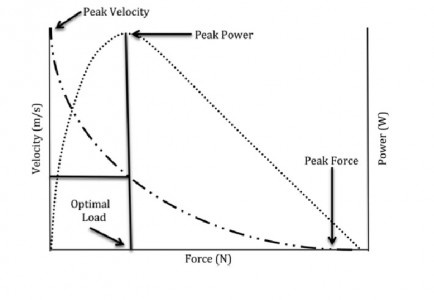
\includegraphics[scale=0.6]{imagenes/OPTIMAL-LOAD-434x300.jpg}
	\caption{Relación entre fuerza y velocidad, punto de máxima potencia 'Optimal Load' o 'Peak Power'.}
	\label{PeakPower}
\end{figure}
\\
\\

La carga seleccionada para el desarrollo óptimo de la potencia suele ser entre el 30-45\% del 1RM, aunque este porcentaje puede variar \cite{Cormie}.

\section{Objetivos}

Los objetivos perseguidos en el desarrollo del proyecto son los siguientes:

\begin{enumerate}
	\item  \textbf{La creación de una aplicación que facilite la labor de un entrenador personal a la hora de realizar, medir y valorar los progresos de un usuario a lo largo del tiempo.} \\
			Probar la viabilidad del desarrollo de una aplicación de salud y deporte utilizando dispositivos de propósito general con sensores, en lugar de un IMU específico.

	\item  \textbf{Investigación de métodos de posicionamiento y rastreo en un escenario real y 3D.} \\
			Realizando la calibración de sensores de bajo coste con el fin de reducir el ruido y el error innato de los sensores.

	\item \textbf{Aplicar los conocimientos adquiridos sobre ingeniería del software.} \\
			Se ha perseguido la aplicación de los conocimientos adquiridos durante el grado en el desarrollo de software en un proyecto real.

	\item  \textbf{Elaboración de un prototipo funcional del proyecto.} \\
			Se persigue la implementación de una aplicación funcional, una aplicación que será instalada en el smartwatch, que provea de los datos y mediciones de la realización del ejercicio. Y otra aplicación instalada en el smartphone que se encargará de recopilar los datos, procesarlos y mostrarlos.
\end{enumerate}

\section{Estructura}

Este documento se encuentra dividido en ocho capítulos. Los cuales desarrollan:

\begin{enumerate}
	\item \textbf{Capítulo 1: Introducción.} Es el capítulo en el que se encuentra esta sección, está formado por tres secciones. La primera llamada Motivación 1.1 describe que es un entrenamiento basado en potencia y los beneficios que se obtiene de este tipo de entrenamiento. La segunda sección denominada Objetivos 1.2, contiene un resumen de los objetivos que se pretenden alcanzar con el desarrollo de este proyecto. La última sección denominada Estructura 1.3, presenta la estructura de los capítulos del presente documento así como una breve descripción de sus contenidos.
	\item \textbf{Capítulo 2: Estado del arte} Este capítulo se organiza en tres apartados. El primero, llamado Estado del mercado 2.1 define el estado actual del mercado de tecnologías que permiten realizar mediciones de entrenamientos basados en potencia. El segundo capítulo denominado Tecnologías 2.2 contiene una breve descripción de las tecnologías que nos van a permitir el desarrollo de este proyecto. Por último la sección llamada Sensores de movimiento en Android 2.3 trata sobre los principales tipos de sensores relacionados con el movimiento que se encuentran disponibles en Android.
	\item \textbf{Capítulo 3: Especificación de requisitos} En este capítulo encontramos los distintos tipos de requisitos que debe cumplir el sistema. Se encuentra estructurado en tres secciones. Requisitos funcionales 3.1, los cuales definen funciones del sistema. En la segunda sección encontramos los Requisitos no funcionales 3.2, los cuales contienen restricciones del sistema relacionadas con el diseño o la implementación. Finalmente, encontramos la sección Requisitos de información 3.3, los cuales hacen referencia a información que debe ser almacenada en el sistema.
	\item \textbf{Capítulo 4: Planificación} Este capítulo se organiza en dos apartados. El primero llamado Planificación 4.1, contiene la planificación general del proyecto, haciendo uso de metodologías ágiles. El segundo apartado denominado Coste del proyecto 4.2, contiene un escueto presupuesto sobre el desarrollo del proyecto.
	\item \textbf{Capítulo 5: Análisis de los datos} Este capítulo está formado por 5 secciones. La primera denominada Introducción al problema 5.1, nos habla sobre porque es importante tratar los datos de los sensores en el desarrollo de este proyecto. La segunda sección llamada Cálculo de la velocidad 5.2, describe como se obtiene la velocidad a partir de la aceleración. La tercera sección denominada Calibración de los sensores 5.3, comenta tres técnicas diferentes para conseguir eliminar la componente gravitacional de la aceleración. La sección Pruebas de calibración 5.4, pone las técnicas descritas en el apartado anterior a prueba. Finalmente, la sección Eliminación de ruido mecánico 5.5, describe un método para eliminar parcialmente el ruido mecánico de los sensores.
	\item \textbf{Capítulo 6: Diseño} En este capítulo se encuentran 5 secciones. La primera, Diseño del sistema 6.1, describe la arquitectura general del sistema. La segunda, Diagrama de clases de la aplicación móvil 6.2, describe atributos, métodos y relaciones de la aplicación móvil. La tercera, Diagrama de clases de la aplicación wear 6.3, describe atributos, métodos y relaciones de la aplicación wear. La cuarta sección denominada Casos de uso 6.4, contiene los distintos casos de uso de los usuarios en el sistema. Finalmente, la sección Diseño de la base de datos 6.5, describe la estructura de la base de datos.
	\item \textbf{Capítulo 7: Implementación} Formado por 3 secciones. La primera llamada Hito 1: Asistente entrenamiento potencia 7.1, describe los pasos realizados para implementar el asistente de entrenamiento. La segunda, denominada Hito 2: Uso del servidor, describe los pasos realizados para implementar la conexión con el servidor. Finalmente, la sección Capturas 7.3, contiene capturas sobre la aplicación.
	\item \textbf{Capítulo 8: Conclusiones y trabajo futuro} Realiza un análisis sobre los objetivos buscados, conseguidos y los resultados del proyecto. Además de exponer cual será el trabajo futuro.
\end{enumerate}

\chapter{Estado del arte}

\section{Estado del mercado}

Existen tres herramientas principales a la hora de monitorizar un entrenamiento basado en potencia:

\subsubsection*{Encoder Lineal}

Un encoder lineal es un dinamómetro que, aplicado al deporte, se utiliza para realizar una medición directa y contínua del espacio recorrido y el tiempo de movimiento de una carga conocida. Pudiendo utilizarse así para calcular la potencia, fuerza o velocidad \cite{encoder}.
\\
\\
Son muy fiables y precisos, pero presentan también algunos inconvenientes. El principal inconveniente es su precio, que puede ser realmente elevado. Por lo su venta no va dirigida a usuarios particulares, si no a profesionales. Además requere de personal cualificado para su uso e interpretación.

\subsubsection*{Push Band}

Push Band es un dispositivo wearable IMU, que conectado a una aplicación permite la monitorización del entrenamiento. Además, dispone de una interfaz web, accesible desde cualquier plataforma\cite{push}.
\\
\\
Si bien su coste no es tan elevado, también presenta inconvenientes. El principal de ellos es que está disponible solo para iOS.

\subsubsection*{Beast Sensor}

Beast Sensor es también un dispositivo wearable IMU, que se conecta a través de una aplicación móvil (disponible en iOS y Android) y es usada para monitorizar el ejercicio\cite{beast}. Además también presenta una interfaz web donde se puede consultar la información de una cuenta.
\\
\\
Las diferencias entre Beast Sensor y Push Band son mínimas, su principal diferencia es que Beast funciona en Android mientras que Push no. Se debe destacar que, tanto estas dos herramientas como los encoders lineales hacen uso de dispositivos de propósito específico, que el usuario debe adquirir expresamente si desea monitorizar su entrenamiento.
\\
Por ello surge este proyecto, con el fin de poder realizar la monitorización del entrenamiento con un dispositivo de propósito general. Como son los smartwatches con Android Wear.


\section{Tecnologías}

\subsection{Android}

Android es un sistema operativo móvil desarrollado por Google y basado en el kernel de Linux, diseñado principalmente para dispositivos móviles y otros dispositivos de pantalla táctil, como smartphones, smartwatches y tabletas. Originalmente fue desarrollado por Android Inc. , la cual fué posteriormente adquirida por Google. Android es además un sistema multiplataforma, lo cual lo ha hecho adquirir el gran éxito y popularidad de la que goza hoy en día.

\subsubsection{Arquitectura de Android}

\begin{figure}[H]
	\centering
	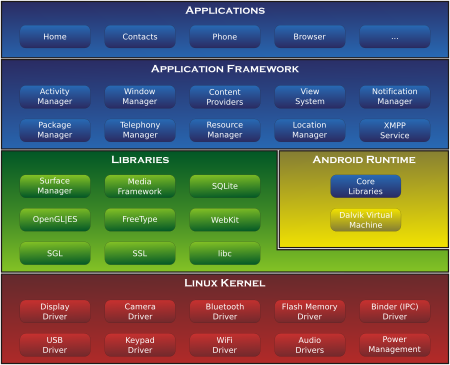
\includegraphics[scale=0.7]{imagenes/capasandroid.png}
	\caption{Arquitectura del SO Android}
	\label{Arquitectura del SO Android}
\end{figure}
\noindent
La arquitectura de Android se encuentra formada por capas. Como podemos apreciar en la figura superior, en la base de la pila se encuentra el kernel de Linux. Construido en C principalmente, es el encargado de la gestión de la memoria, servicios de seguridad y de dar soporte a los controladores.
\\
\\
La capa inmediatamente superior, es la capa del framework de aplicación, la cual incluye librerias y la denominada 'Android Runtime'.
\\
Las librerías son nativas, escritas en C y precompiladas. Entre ellas se destacan:
\begin{itemize}
\item SSL: Proporciona servicios de seguridad y encriptación.
\item SQLite: Motor de bases de datos relacionales.
\item WebKit: Ofrece soporte para el navegador web y su vista webview.
\end{itemize}
\\
\\
El entorno de ejecución o 'Android Runtime' , basado en la máquina virtual de Java, recibe el nombre de Dalvik. La máquina virtual será la encargada de compilar y ejecutar de forma nativa fragmentos de código denominados tazas de código, cada vez que una aplicación es lanzada. Optimizando de esta manera los recursos del sistema y delegando al kernel el threading y el manejo de memoria a bajo nivel.
\\
\\
En la capa inmediatamente superior encontramos el marco de aplicación o 'Application Framework', el cual ofrece una plataforma a las aplicaciones, incluyendo librerías Java. Entre ellas, las más importantes son:
\begin{itemize}
\item Activity Manager. Manejador destinado al ciclo de vida de las actividades.
\item Views. Conjunto de vistas.
\item Location Manager. Proporciona servicios de localización a aplicaciones.
\item Content Provider. Concede accesos a datos de otras aplicaciones.
\item Notification Manager. Facilita el soporte para mostrar notificaciones a las distintas actividades.
\end{itemize}
\\
En la capa superior de abstracción, encontramos la placa de aplicación. La cual engloba a todas las aplicaciones que se encuentren instaladas en el dispositivo.
\\
\subsubsection{Tareas y pila de actividades}

Una aplicación generalmente esta formada por una serie de actividades, las cuales son necesarias para el correcto funcionamiento de la aplicación. Por norma general, cada actividad debe estar diseñada en torno a una clase de acción que puede realizar el usuario y se deben poder comunicar con otras actividades, creándolas y enviando información entre ellas. Pudiendo incluso darse el caso de que una actividad inicie una actividad existente en otra aplicación del dispositivo, lo cual otorga una gran versatilidad.
\\
\\
Podemos definir una tarea como la colección de actividades cuyo objetivo o finalidad es común. Dichas actividades son organizadas en la pila de actividades, la cual se va rellenando en el orden en el que se abre cada actividad.
\begin{figure}[H]
	\centering
	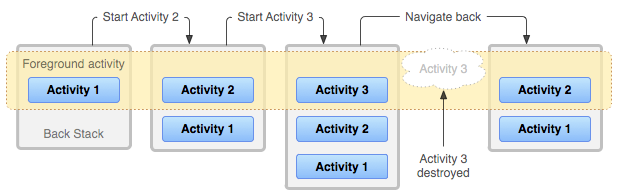
\includegraphics[width=\textwidth]{imagenes/activityStack.png}
	\caption{Pila de actividades de Android.}
	\label{Pila de avtividades}
\end{figure}
\\
\\
En la figura anterior, podemos ver el contenido de la pila en base a diferentes acciones. Cuando creamos una nueva actividad, la actividad anterior sigue mantenida en la pila de actividades, ocupando así la nueva actividad creada la cima de la pila. Al pulsar el botón hacia atrás o destruir una actividad, la actividad que ocupaba la segunda posición en la pila, queda en el tope de la pila y se vuelve a mostrar dicha actividad, liberando los recursos que estaba consumiendo la actividad anterior.
\\
Cuando la pila de actividades se encuentra vacía, la tarea deja de existir y sus recursos son liberados totalmente. Además, si cambiamos a otra actividad de otra aplicación o volvemos a la pantalla de inicio, las actividades de la pila pasaran a segundo plano, deteniéndose, pero la pila de retroceso permanecerá intacta.
%************************************************
\subsection{Android Wear}

Android Wear es una versión del sistema operativo de Google, Android. Desarrollado para usarse como sistema operativo en smartwatches. El sistema operativo fue lanzado por Google en 2014 y puede ser conectado con dispositivos Android a partir de su versión 4.3 o en iPhone a partir de iOS 9. Siendo posible que la funcionalidad varíe en función de la plataforma y versión del sistema operativo.
\\
\\
Actualmente se encuentra en la versión 2.0 en la cual se da mayor independencia al dispositivo wear con respecto al smartphone. Otorgandole así mayor autonomía.
\\
La mayor diferencia entre el ecosistema Android y Android Wear se aprecia en las actividades, tienen un conjunto diferente de eventos que se asocian con el sistema operativo, los más destacados son:
\begin{itemize}
\item Cuando cambia la hora.
\item Cuando llega una notificación.
\item Cuando la intensidad del brillo de la pantalla cambia.
\end{itemize}

\subsection{GoogleAPIClient}
La clase GoogleApiClient es el punto de enlace para los servicios de integración de Google Play (\textit{Google Play Services}). Es decir, cualquier aplicación que quiera hacer uso de alguna API de los servicios de Google, deberá instanciar un cliente de dicha clase en la aplicación.
\\
\\
La clase dispone de una gran multitud de métodos. Algunos requieren que el el cliente GoogleApiClient este conectado, otros se encolan cuando no hay una conexión establecida. Pero para poder ejecutar cualquier operación, debe existir una conexión\cite{GoogleApiClient}.
\subsection{DataAPI}

Es una Api que forma parte de los servicios de \textit{Google Play Services}, los cuales proveen a las aplicaciones de un canal de comunicación adicional, en este caso, para un dispositivo wearable.
La Api Data Layer consiste en una serie de objetos que pueden ser utilizados para enviar y sincronizar datos, en conjunto con los \textit{'listeners'}, para establecer una comunicación.
En nuestro caso vamos a utilizar la Api para establecer un canal de comunicación entre el dispositivo Wearable y el móvil construido sobre el estándar Bluetooth \cite{DataAPI}.

\begin{figure}[H]
	\centering
	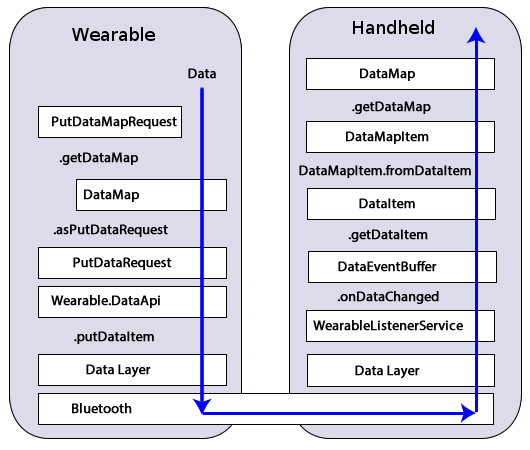
\includegraphics[scale=0.5]{imagenes/dataApi.png}
	\caption{Estructura de la capa DataApi.}
	\label{DataApi}
\end{figure}
\noindent
Para emplear esta API, se debe disponer de una versión de Android igual o superior a la 4.3 (API 18) en el dispositivo wear. La primera versión disponible de Android Wear está basado en Android 4.4.2 KitKat (API 19), por lo que es compatible con todos los dispositivos Android Wear. Además, cabe destacar que se debe de utilizar la última versión de Google Play services \cite{playServices}.


\subsection{Firebase}

Firebase \cite{firebase} es una aplicación web y móvil del tipo BaaS (Backend-as-a-Service), es decir ofrece funcionalidades propias de un servidor por medio de una interfaz. Permitiendo a las aplicaciones conectarse y sincronizarse con un servidor de una manera rápida y sencilla sin necesidad de implementar una API Rest.
\\
\\
En su esencia, es principalmente una base de datos en tiempo real, la cual hace uso del protocolo WebSockets en lugar de HTTP. Y su principal ventaja es que todos los clientes de la aplicación en tiempo real sincronizan sus datos, de manera que todos los clientes de la base de datos los reciben de manera instantánea.
\\
Utiliza un modelo de base de datos NoSQL. Los datos se almacenan en formato JSON. Y como tal ofrece diferentes funcionalidades en comparación con una base de datos relacional, siendo la velocidad su mayor ventaja.
\\
\\
Además de brindar una base de datos, provee una amplia lista de funcionalidades , sus principales son:
\begin{itemize}
\item Almacenamiento de archivos. Permite almacenar archivos en '\textit{Google Cloud Storage}' de forma directa desde el cliente.
\item Autenticación. Ofrece un sistema de autenticación por medio de email/contraseña, además soporta autenticación en base a '\textit{OAuth2}' con multitud de servicios, como Google, Facebook, Twitter y Github.
\item Servicio de alojamiento. Permite almacenar y servir archivos estáticos utilizando el protocolo HTTP/2.
\end{itemize}


\subsection{Sensores}

Se define como sensor a un elemento o dispositivo electrónico, que detecta eventos o cambios en el entorno en el que se encuentran y envían la información de dicho evento a otro dispositivo electrónico.
\\
\\
La sensibilidad es definida como el ratio entre la señal de salida y la magnitud de la propiedad medida. La mayoría de sensores tienen una función de transferencia lineal.

\subsubsection{Desviaciones de los sensores}

Los sensores no pueden replicar una función de transferencia ideal. Presentando las diferentes fluctuaciones:

\begin{itemize}
\item El rango de la señal de salida esta limitado, soliendo obedecer normalmente a un Vpp. Por lo que la salida del sensor alcanzará eventualmente un mínimo y un máximo.

\item La sensibilidad práctica difiere del valor especificado. Denominado como error de sensibilidad.

\item Si la señal de salida difiere del valor correcto por una constante y, se dice que el sensor posee un error de \textit{\textbf{offset}} (desplazamiento) o error bias.

\item La no linearidad es la desviación de la función de transferencia de un sensor.

\item La desviación causada por cambios rápidos en la propiedad que se esta midiendo se conoce como error dinámico.

\item Si la señal de salida cambia de manera muy lenta, independientemente de la variación de la propiedad medida, dicho fenómeno es conocido como \textit{\textbf{drift}} (desvío).

\item El ruido es una desviación aleatoria de la señal que varía con respecto al tiempo.

\item Los sensores con una señal de salida digital, la salida es esencialmente una aproximación de la propiedad medida. Dicho fenómeno es llamado error de quantización.

\item Cuando la señal es monitorizada digitalmente, la frecuencia de muestreado puede causar errores dinámicos, o si la entrada de datos cambia periódicamente a otra frecuencia, puede producir errores de \textit{antialising} (acoplo).

\end{itemize}

\section{Sensores de movimiento en Android}

La Api de Android provee de varios sensores con el fin de poder monitorizar el movimiento del dispositivo.
\\
\\
Android provee de sensores basados en software o hardware. Los sensores software como la gravedad, vector de rotación, contador de pasos etc, han de ser implementados usando sensores hardware (acelerómetros, giroscopios y magnetómetros).
\\
Actualmente, la gran mayoría de dispositivos Android tradicionales contienen acelerómetros, giroscopios y magnetómetros. Sin embargo no todos los dipositivos Android Wear disponen de estos tres sensores, siendo el caso más común que dispongan de acelerómetro y giroscopio únicamente \cite{SensorGoogle}.

\subsection{Acelerómetro}

Un acelerómetro es un dispositivo que mide vibración o aceleración propia de una estructura. Siendo la aceleración el ratio del cambio de velocidad con respecto al tiempo.
\\
La fuerza causada por las vibraciones de un cambio en el movimiento (aceleración) causa que la masa mueva el material piezoeléctrico generando una carga que es proporcional a la fuerza que experimenta (Fuerza de la gravedad incluida) .

\begin{figure}[H]
	\centering
	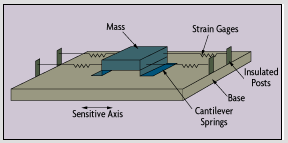
\includegraphics[scale=0.7]{imagenes/piezoelectrico.png}
	\caption{Acelerómetro piezoeléctrico}
	\label{Accelerometer}
\end{figure}
\noindent
Los acelerómetros \textit{multi-axis} (varios ejes) son capaces de detectar magnitudes y direcciones de la propia aceleración como un vector cuantitativo \cite{WikipediaAccelerometer}.


\subsubsection{Acelerómetro en Android}

El acelerómetro mide la aceleración aplicada al dispositivo móvil, incluyendo la fuerza de la gravedad. Siguiendo el estándar de coordenadas que podemos apreciar en la siguiente figura:

\begin{figure}[H]
	\centering
	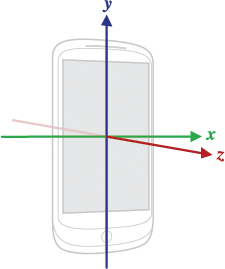
\includegraphics[scale=0.8]{imagenes/axis_device.png}
	\caption{Sistema de coordenadas relativo a la API de los sensores.}
	\label{Sistema de coordenadas sensores}
\end{figure}
\noindent
Es el sensor principal que se debe monitorizar para realizar un seguimiento de movimiento. Puesto que esta presente en todos los dispositivos móviles comerciales y tiene un consumo de energía de hasta 10 veces menor que el resto de sensores.
\noindent
La API provee de una serie diferente de posibilidades para el uso del acelerómetro \cite{GoogleAcel}:

\begin{table}[H]
\centering
    \begin{tabular}{p{5.0cm} p{2.0cm} p{5.0cm} p{2.0cm}}%{|l{2cm}|l|l{2cm}|c|}
    \hline
    Sensor & Estructura de Datos & Descripción & Unidades \\ \hline
    \\ TYPE\_ACCELEROMETER (API 3) & Vector[3] & Fuerza de aceleración a lo largo de los 3 ejes. Incluyendo la gravedad. & m/s\^2 \\\\ \hline
    TYPE\_ACCELEROMETER\\\_UNCALIBRATED (API 26) & Vector[3] & La aceleración medida a lo largo de los 3 ejes sin ningún tipo de desviación bias.  & m/s\^2 \\\\ \hline
    \\TYPE\_GRAVITY (API 9) & Vector[3] & La aceleración producida por la fuerza de la gravedad. & m/s\^2 \\\\ \hline
    TYPE\_LINEAR\\\_ACCELERATION (API 9) & Vector[3] & La aceleración a lo largo de los 3 ejes. Excluyendo la gravedad & m/s\^2 \\\\ \hline
    \end{tabular}
\end{table}

\subsection{Giroscopio}

Un giroscopio es un dispositivo usado para medir el grado de rotación en radianes por segundo a lo largo de un eje de coordenadas. Es decir, son dispositivos que miden la velocidad angular.
\noindent
En los últimos años, ha aumentado el empleo de giroscopios de estructura vibrante en todo tipo de industrias, como móviles, vehículos, fotografía, etcétera.

\subsubsection{Giroscopios de estructura vibrante}

Los giroscopios de estructura vibrante miden la velocidad angular de la fuerza causada por el efecto Coriolis aplicada a un elemento en vibración. Por lo que la precisión de la velocidad angular medida difiere dependiendo del material. En la siguiente figura se puede apreciar la estructura:

\begin{figure}[H]
	\centering
	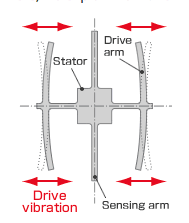
\includegraphics[scale=0.7]{imagenes/gyro.png}
	\caption{Giroscopio de estructura vibrante.}
	\label{Giroscopio de estructura vibrante}
\end{figure}

\subsubsection{Giroscopios en Android}
\\
El giroscopio mide el grado de rotación a lo largo de los 3 ejes de coordenadas del dispositivo, siguiendo el mismo sistema de coordenadas de la API. La rotación es positiva en el sentido anti\-horario.

\begin{table}[H]
\centering
    \begin{tabular}{p{5.0cm} p{2.0cm} p{5.0cm} p{2.0cm}}%{|l{2cm}|l|l{2cm}|l|}
    \hline
    Sensor & Estructura de Datos & Descripción & Unidades \\ \hline
    \\TYPE\_GYROSCOPE (API 3) & Vector[3] & Ratio de rotación 3-axis. & rad/s \\\\ \hline
    TYPE\_GYROSCOPE\\\_UNCALIBRATED (API 18) & Vector[3] & Ratio de rotación 3-axis.Sin compensación drift. & rad/s \\\\ \hline
    TYPE\_ROTATION\_VECTOR (API 9) & Vector[3] & Rotación vector componente a lo largo de los ejes (eje * Sin(O/2)) & Sin unidades \\ \hline
    \end{tabular}
\end{table}
\noindent
Por defecto los giroscopios también proveen de datos sin ningún tipo de filtrado, por lo que la varianza 'bias' y el ruido inherente están presentes en los datos obtenidos. El tipo de sensor \textbf{TYPE\_GYROSCOPE} provee de datos con compensación 'bias'. El tipo de sensor \textbf{TYPE\_GYROSCOPE\_UNCALIBRATED} no provee ningún tipo de calibración, obedeciendo a la siguiente relación para cada eje.
\\

\[calibrated_x ~= uncalibrated_x - bias_estimate_x\]



\subsection{Magnetómetro}

Un magnetómetro es un instrumento cuya finalidad es medir la intensidad de un campo magnético. Pudiendo  dividirse en dos tipos:

\begin{itemize}
\item Magnetómetros escalares. Los cuales miden la fuerza total de los campos magnéticos bajo los que se encuentran. Es decir, miden la sumatoria de la fuerza magnética en todas las direcciones.

\item Magnetómetros vectoriales. Tienen la capacidad de medir la intensidad del campo magnético bajo los que se encuentran en una dirección en concreto.
\end{itemize}

\begin{figure}[H]
	\centering
	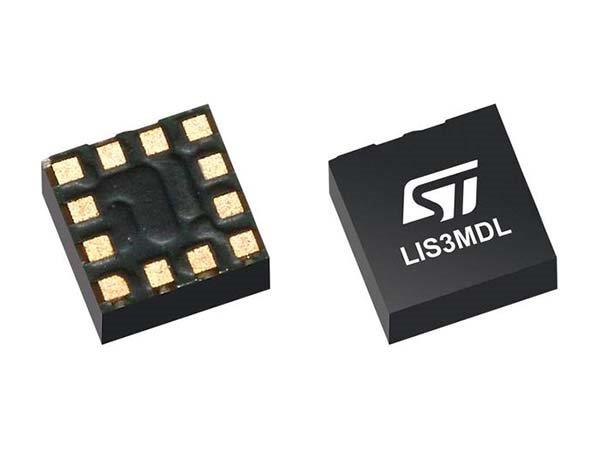
\includegraphics[scale=0.5]{imagenes/magnetometer.jpg}
	\caption{Magnetómetro.}
	\label{Magnetometro}
\end{figure}

\subsubsection{Magnetómetro en Android}

El magnetómetro en Android mide cambios en la intensidad del campo magnético terrestre .

\begin{table}[H]
\centering
    \begin{tabular}{p{5.0cm} p{2.0cm} p{5.0cm} p{2.0cm}}%{|l{2cm}|l|l{2cm}|l|}
    \hline
    Sensor & Estructura de Datos & Descripción & Unidades \\ \hline
    TYPE\_MAGNETIC\\\_FIELD (API 3) & Vector[3] & Campo geomagnético  3-axis. & $\mu$T \\\\ \hline
    TYPE\_MAGNETIC\\\_FIELD\_UNCALIBRATED (API 18) & Vector[6] & Campo geomagnético  3-axis sin calibración de 'Iron'  Estimación bias de 'Iron' 3-axis  & $\mu$T \\ \\ \hline
    \end{tabular}
\end{table}
\noindent
El tipo \textbf{TYPE\_MAGNETIC\_FIELD} es similar es calibrado siguiendo la siguiente regla:

\[calibrated_x ~= uncalibrated_x - bias_estimate_x\]
\noindent
Se debe tener en cuenta que los sensores no calibrados pueden contener desviación bias, pero contienen menos saltos en la frecuencia de muestreo, por lo que dichos sensores proveen datos más frecuentemente y consecuentemente, más fiables en cuanto a frecuencia.

%
\chapter{Especificación de requisitos}

Todo software es creado con el fin de cumplir un servicio o una necesidad. Y como en todo proyecto de software, los requisitos deben ser especificados en la fase previa al desarrollo con el fin de dar cobertura a todas las necesidades del usuario.
\\
\\
Se entiende como requisito una funcionalidad o requerimiento que un usuario necesita para poder poder cumplir una necesidad en concreto o resolver un problema.
\\
\\
En este capítulo se analizan los distintos requisitos del sistema que vamos a detallar en este documento. Se encuentra estructurado en tres secciones. Requisitos funcionales 3.1, los cuales definen funciones del sistema. En la segunda sección encontramos los Requisitos no funcionales 3.2, los cuales contienen restricciones del sistema relacionadas con el diseño o la implementacion. Finalmente, encontramos la sección Requisitos de información 3.3, los cuales hacen referencia a información que debe ser almacenada en el sistema.

\section{Requisitos funcionales}

Los requisitos funcionales son los encargados de definir una función del sistema. De manera que se cubran todas las necesidades de los usuarios.\\
\\
El sistema cuenta con los siguientes requisitos funcionales:

\textbf{RF-1. Autenticación:} Control de usuarios.
\\

\begin{itemize}

\item \textbf{RF-1.1} El usuario debe poder darse de alta en la aplicación.
\item \textbf{RF-1.2} El usuario debe poder inicar sesión en la aplicación.
\item \textbf{RF-1.3} El usuario debe poder recuperar sus credenciales.
\end{itemize}
\\
\\\\
\textbf{RF-2. Control:} Control del ejercicio.
\\
\\
\begin{itemize}
\item \textbf{RF-2.1} Se debe poder controlar el inicio del ejercicio/repetición.
\item \textbf{RF-2.2} Se debe poder controlar el final del ejercicio/repetición.
\item \textbf{RF-2.3} El usuario puede seleccionar el tipo de ejercicio.
\item \textbf{RF-2.4} El usuario debe ser capaz de realizar una nueva serie.
\item \textbf{RF-2.5} El usuario debe ser capaz de introducir el peso con el que esta realizando el ejercicio.
\end{itemize}
\\\\
\\
\textbf{RF-3. Visualización:} Representación de la información.
\\
\begin{itemize}
\item \textbf{RF-3.1} El usuario podrá consultar la potencia realizada.
\item \textbf{RF-3.2} Visualizar el contenido de un dia en concreto.
\end{itemize}
\\

\section{Requisitos no funcionales}

Los requisitos no funcionales describen restricciones del sistema que se relacionan con el diseño o la implementación del proyecto.
\\
\\
A continuación se describen los requisitos no funcionales de este proyecto:
\\
\begin{itemize}
\item \textbf{RNF-1}. Ambas aplicaciones han de ser implementadas en Java.
\item \textbf{RNF-2}. El envío de datos debe ser en tiempo real.
\item \textbf{RNF-3}. La visualización debe ser creada en tiempo real, durante la realización del ejercicio.
\item \textbf{RNF-4}. El sistema deberá enviar la información al servidor, con el fin de no ocupar almacenamiento local en el dispositivo.
\item \textbf{RNF-5}. El sistema deberá almacenar la información en local si no dispone de conexión a Internet.
\item \textbf{RNF-6}. La frecuencia de muestreo debe ser ajustada para usar la menor cantidad de memoria posible.
\item \textbf{RNF-7}. Los datos deben ser tratados para conseguir la máxima precisión posible.
\end{itemize}
\\
\\
\section{Requisitos de información}

Los requisitos de información se refieren a la información que es imprescindible almacenar en el sistema.
\\
\\
A continuación vamos a describir los requisitos de información del sistema:
\\
\\
\begin{itemize}
    \item \textbf{RI-1} Almacenamiento de credenciales: correo electrónico y contraseña.
    \item \textbf{RI-2} Historial de entrenamiento del usuario.
\end{itemize}

%
\chapter{Planificación}

En este capítulo se pueden encontrar dos secciones, en la primera se aborda la Planificación 4.1, para el desarrollo del proyecto y en la segunda el Coste del proyecto 4.2, la cual contiene un presupuesto sobre el coste del desarrollo de este proyecto.

\section{Planificación}

Se ha realizado la planificación del proyecto en base a una metodología ágil. Obteniendo así una mayor flexibilidad en el desarrollo, para ello se han realizado historias de usuario, definiendo en ellas la funcionalidad mínima para el correcto funcionamiento del sistema, iterando desde las tareas de máxima prioridad hasta las de prioridad más baja.
\\
Se han desarrollado dos grandes hitos:
\begin{itemize}
\setlength\itemsep{0pt}
    \item \textbf{1. Asistente entrenamiento potencia}
    \item  \textbf{2. Uso de un servidor}
\end{itemize}
\noindent
Se han conseguido desarrollar los dos hitos, a falta de mejorar la interfaz de cara a una mejor experiencia del usuario. %Puesto el resultado obtenido desarrollado buscando la funcionalidad, quedando pendiente dicha mejora.
\\
\\
A continuación se van a detallar los hitos:
\subsection{Asistente entrenamiento potencia}
\begin{adjustbox}{margin=3.5ex 16ex 3.5ex 3.5ex,center}
	\begin{forest} for tree={
	    growth parent anchor=south,
	    parent anchor=south,
	    child anchor=north,
	    edge path={none},
	    l sep=.25cm,
	}
	%
	[Asistente entrenamiento potencia, goal, name=agoal
	    [Aplicación Android Wear, activity
	        [1. Conexión con la aplicación Android, task
	       	[2. Recolección de los datos de los sensores, task
	        [3. Envío de los datos a la aplicación Android, task
	        [4. Mejora de la interfaz de inicio y fin de serie, task
	        ] ] ] ] ]
	    [Aplicación Android, activity
	        [1. Conexión con la aplicación wear, task
			[2. Mostrar la lista de ejercicios disponibles, task
	        [3. Recepción de los datos desde la aplicación Wear, task
	        [4. Tratamiento de los datos recibidos, task
	        [5. Calculo de la velocidad y de la potencia, task
	        [6. Representación de cada serie de manera visual, task
	        ] ] ] ] ] ] ] ]
	%
	\end{forest}
\end{adjustbox}
\noindent
Una vez finalizado este hito, se ha conseguido una arquitectura totalmente operativa para realizar y monitorizar un entrenamiento basado en potencia en tiempo real. Por lo que el objetivo principal del proyecto se podría dar por conseguido.
\\
\\
En el siguiente hito dotaremos al proyecto de funcionalidades adicionales, que mejoren el funcionamiento del mismo y amplien sus capacidades.
\\
\\
Para ello dotaremos a nuestro sistema de conexión a un servidor, el cual ampliará las capacidades de la aplicación de cara al usuario y también el propio sistema.
\\
\subsection{Uso de un servidor}

\begin{adjustbox}{margin=3.5ex 6ex 3.5ex 3.5ex,center}

	\begin{forest} for tree={
	    growth parent anchor=south,
	    parent anchor=south,
	    child anchor=north,
	    edge path={none},
	    l sep=.25cm,
	}
	%
	[Asistente entrenamiento potencia, goal, name=agoal
	    [Servidor, activity
	        [1. Conexión con la aplicación Android, task
	       	[2. Creación de usuarios, task
	        [3. Autenticación de los usuarios, task
	        [4. Recepción y envío de datos a la aplicación Android, task
	        ] ] ] ] ]
	    [Aplicación Android, activity
	        [1. Conexión con el servidor, task
			[2. Envío de credenciales al servidor, task
	        [3. Envío y recepción de datos al servidor, task
	        [4. Representación de los datos recibidos por el servidor, task
	        ] ] ] ] ] ]
	%
	\end{forest}
\end{adjustbox}
\noindent
Una vez finalizado este hito se ha completado las competencias de este proyecto y su funcionalidad es completa, a falta de una reconstrucción de la interfaz que mejore la experiencia de los usuarios del sistema.

\section{Coste del proyecto}

En esta sección se va a realizar una estimación de los costes materiales y humanos del proyecto tratado en esta memoria.

\subsection*{Costes materiales}

El equipo utilizado para este proyecto consta de:
\\
Ordenador utilizado para el desarrollo, junto al siguiente software:

\begin{itemize}
\setlength\itemsep{0em}
    \item Sistema Operativo: Ubuntu 16.04
    \item Editor de texto: Sharelatex (Online)
    \item IDE: Android Studio
    \item Diseño de programas UML: Visual Paradigm CE
    \item Gestión de versiones: Github
\end{itemize}
\noindent
Además se ha utilizado un móvil Android (Honor 8 lite) y dos smartwatches (Moto 360 y Sony Smartwatch Sport 3).
\\
Por lo tanto los costes materiales son de :
\begin{itemize}
\setlength\itemsep{0em}
    \item Ordenador. Coste total 900€. Con una vida útil estimada de 5 años \cite{lifespan}, tiene un coste anual de 180 euros/año, 15 euros por mes.
    \item Móvil Android. Coste total 200€. Con una vida útil media de 2 años \cite{nytimes}, supone un coste de 100 euros/año, 8,3 euros/mes.
    \item Dispositivos wearable. Coste total 150 euros y 120 euros respectivamente. Con un ciclo de vida media de dos años \cite{authority}, suponen un coste de 75 euros/año y 60 euros/año y, consecuentemente, un coste de 6,25 euros/mes y 5 euros/mes.
\end{itemize}

\subsection*{Costes humanos}

Se ha realizado un seguimiento de horas empleadas en cada tarea para estimar los costes humanos del proyecto. Para estimar el coste, se ha teniendo en el salario medio de un programador junior en España \cite{infojob}, siendo de 19.787 euros/año, el coste por hora es de 8,83 euros.
% Please add the following required packages to your document preamble:
% \usepackage[table,xcdraw]{xcolor}
% If you use beamer only pass "xcolor=table" option, i.e. \documentclass[xcolor=table]{beamer}
\begin{table}[H]
\centering
\caption{Costes humanos del proyecto}
\label{Costes humanos del proyecto}
\begin{tabular}{llll}
\hline
\multicolumn{1}{|l|}{Nombre de la tarea}              & \multicolumn{1}{l|}{Número de horas} & \multicolumn{1}{l|}{Coste por hora}  & \multicolumn{1}{l|}{Total (euros)} \\ \hline
\multicolumn{1}{|l|}{Estudio previo}                  & \multicolumn{1}{l|}{120}             & \multicolumn{1}{l|}{8,83 euros/hora} & \multicolumn{1}{l|}{1059,6}        \\ \hline
\multicolumn{1}{|l|}{Estudio de los requisitos}       & \multicolumn{1}{l|}{8}               & \multicolumn{1}{l|}{8,83 euros/hora} & \multicolumn{1}{l|}{70,64}         \\ \hline
\multicolumn{1}{|l|}{Estudio del mercado}             & \multicolumn{1}{l|}{8}               & \multicolumn{1}{l|}{8,83 euros/hora} & \multicolumn{1}{l|}{70,64}         \\ \hline
\multicolumn{1}{|l|}{Planificación}                   & \multicolumn{1}{l|}{8}               & \multicolumn{1}{l|}{8,83 euros/hora} & \multicolumn{1}{l|}{70,64}         \\ \hline
\multicolumn{1}{|l|}{Desarrollo del Hito 1}           & \multicolumn{1}{l|}{240}             & \multicolumn{1}{l|}{8,83 euros/hora} & \multicolumn{1}{l|}{2119,2}        \\ \hline
\multicolumn{1}{|l|}{Desarrollo del Hito 2}           & \multicolumn{1}{l|}{40}              & \multicolumn{1}{l|}{8,83 euros/hora} & \multicolumn{1}{l|}{353,2}         \\ \hline
\multicolumn{1}{|l|}{Elaboraciónde las pruebas}       & \multicolumn{1}{l|}{6}               & \multicolumn{1}{l|}{8,83 euros/hora} & \multicolumn{1}{l|}{52,98}         \\ \hline
\multicolumn{1}{|l|}{Elaboración de la documentación} & \multicolumn{1}{l|}{50}              & \multicolumn{1}{l|}{8,83 euros/hora} & \multicolumn{1}{l|}{441,5}         \\ \hline
Total                                                 & \cellcolor[HTML]{38FFF8}480          & 8,83 euros/hora                       & \cellcolor[HTML]{96FFFB}4240 euros
\end{tabular}
\end{table}
\noindent
Se añaden los costes materiales a los humanos.
% Please add the following required packages to your document preamble:
% \usepackage[table,xcdraw]{xcolor}
% If you use beamer only pass "xcolor=table" option, i.e. \documentclass[xcolor=table]{beamer}
\begin{table}[H]
\centering
\caption{Coste total del proyecto}
\label{Coste total del proyecto}
\begin{tabular}{llllll}
\hline
\multicolumn{1}{|l|}{Descripción}     & \multicolumn{1}{l|}{Tipo Recurso} & \multicolumn{1}{l|}{Coste por hora} & \multicolumn{1}{l|}{Coste mensual} & \multicolumn{1}{l|}{Tiempo}  & \multicolumn{1}{l|}{Total}            \\ \hline
\multicolumn{1}{|l|}{Ordenador}       & \multicolumn{1}{l|}{Material}     & \multicolumn{1}{l|}{-}              & \multicolumn{1}{l|}{15 euros}      & \multicolumn{1}{l|}{3 meses} & \multicolumn{1}{l|}{45 euros}         \\ \hline
\multicolumn{1}{|l|}{Móvil}           & \multicolumn{1}{l|}{Material}     & \multicolumn{1}{l|}{-}              & \multicolumn{1}{l|}{8,3 euros}     & \multicolumn{1}{l|}{3 meses} & \multicolumn{1}{l|}{24,9 euros}       \\ \hline
\multicolumn{1}{|l|}{Moto 360}        & \multicolumn{1}{l|}{Material}     & \multicolumn{1}{l|}{-}              & \multicolumn{1}{l|}{6,25 euros}    & \multicolumn{1}{l|}{3 meses} & \multicolumn{1}{l|}{18,75 euros}      \\ \hline
\multicolumn{1}{|l|}{Sony Smartwatch} & \multicolumn{1}{l|}{Material}     & \multicolumn{1}{l|}{-}              & \multicolumn{1}{l|}{5 euros}       & \multicolumn{1}{l|}{3 meses} & \multicolumn{1}{l|}{15 euros}         \\ \hline
\multicolumn{1}{|l|}{Desarrollo}      & \multicolumn{1}{l|}{Humano}       & \multicolumn{1}{l|}{8,83 euros}     & \multicolumn{1}{l|}{-}             & \multicolumn{1}{l|}{3 meses} & \multicolumn{1}{l|}{4238,5 euros}     \\ \hline
Total                                 &                                   &                                     &                                    &                              & \cellcolor[HTML]{38FFF8}4342,05 euros
\end{tabular}
\end{table}
\noindent
Y por lo tanto, el coste total del proyecto será de 4342,05 euros.

%
\chapter{Análisis de los datos}

Este capı́tulo está destinado al estudio y tratamiendo de los datos. Se encuentra dividido en 5 secciones. La primera denominada Introducción al problema 5.1, nos habla sobre porque es importante tratar los datos de los sensores en el desarrollo de este proyecto. La segunda sección llamada Cálculo de la velocidad 5.2, describe como se obtiene la velocidad a partir de la aceleración. La tercera sección denominada Calibración de los sensores 5.3, comenta tres técnicas diferentes para conseguir eliminar la componente gravitacional de la aceleración. La sección Pruebas de calibración 5.4, pone las técnicas descritas en el apartado anterior a prueba. Finalmente, la sección Eliminación de ruido mecánico 5.5, describe un método para eliminar ruido de los sensores.

\section{Introducción al problema}

Se supone el siguiente escenario. El usuario llevará un dispositivo wearable atado a la muñeca y se debe calcular la potencia desarrollada por el usuario en base a los datos que puede aportar el werable. Como se ha presentado en el capítulo 1 de esta memoria, se deberá calcular la velocidad y la fuerza con el fin de obtener la potencia.
\\
\\
Para calcular la velocidad se procederá a integrar la aceleración y para calcular la fuerza tambien se deberá utilizar la aceleración. Por lo que para el correcto funcionamiento de la aplicación y para que sea lo más precisa posible, se debe calcular con la máxima fiabilidad la aceleración.

\section{Calculo de la velocidad}

En esta sección se va a proceder a calcular la velocidad utilizando la integración matemática. Por lo que previamente, se va a definir la aceleración.
\\
La aceleración se define como la variación de la velocidad por unidad de tiempo. Viene representada por:
\\
\[a = \frac{dv}{dt}\]
\\
Cuando la aceleración no es constante aparece una nueva magnitud denominada '\textit{jerk}'. La constante jerk se define como la variación de aceleración respecto al tiempo. Viene representada por:
\\
\[j = \frac{da}{dt}\]
\\
Por lo que se deduce que jerk es la derivada de la aceleración. Para calcular la aceleración solo se debe integrar.
\\
\[da=j*dt\]
\\
\[\int_{a_{0}}^{a}da=\int_{0}^{\partial t}j*dt\]
\\
\[a - a_{0} = j *\partial t\]
\\
\[a = a_{0} + j *\partial t\]
\\
\\
Por otro lado se tiene que la aceleración es la derivada de la velocidad, por lo que que:
\\
\[a = \frac{dv}{dt}\]
\\
\[dv=a*dt\]
\\
\[dv=a_{0} + j *\partial t\*dt\]
\\
\[\int_{v_{0}}^{v}dv=\int_{0}^{\partial t}(a_{0}*jt)dt\]
\\
\[v-v_{0}=a_{0}*\partial t+\frac{1}{2} j \partial t^{2}\]
\\
Teniendo así finalmente la ecuación de la velocidad:
\\
\textbf{
\[v=v_{0}+a_{0}*\partial t+\frac{1}{2} j \partial t^{2}\]}
\\
\\
Una manera de calcular la velocidad es la integral debajo de la curva, donde la integración es la suma de las áreas de longitud mínima.

\begin{figure}[h]
	\centering
	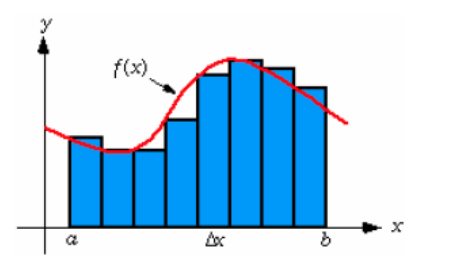
\includegraphics[scale=0.7]{imagenes/velocidad.png}
	\caption{Señal del acelerómetro \cite{nxp}.}
	\label{Calculo velocidad}
\end{figure}

Donde:
\[\int_{a}^{b}f(x) dx=\lim_{n\rightarrow \infty }\sum_{i=1}^{n}f(x_{i})\partial x\]
\\
\[\partial x = \frac{b-a}{n}\]
\\
\[Area_{n} = Muestra_{n} +\frac{\left | Muestra_{n}-Muestra_{n-1} \right |}{2} * T\]
\\
\\
\section{Calibración de los sensores}

Los sensores aportan datos con diferentes ruidos y fluctuaciones como se pudo ver en la sección 2.2 de esta memoria. En este apartado se va a tratar de compensar y calibrar el acelerómetro.
\\
La salida del acelerómetro por norma general varía entre 0V y Vdd, y dicha salida es interpretada por un comparador (A/D). Por lo tanto el valor 0 de la aceleración deberá corresponder con Vdd/2.
\\
Un acelerómetro por defecto esta sometido a la fuerza de la gravedad, así que por defecto la gravedad sobre el eje 'Y' será (situando el sistema de coordenadas sobre el eje de la tierra):
\\
\[g = 9.81 m/s^{2}\]
\\
Por lo que será necesario compensar la aceleración con el fin de eliminar este valor, para ello se van a comparar y aplicar tres técnicas con el fin de averiguar cuál nos ofrece unos datos más precisos.

\subsection{Compensación gravitatoria utilizando Sensor Fusion}

\textbf{Sensor Fusion} se define como el uso de varios sensores con el fin de incrementar la precisión de las mediciones.
\\
\\
En este caso, se va a utilizar el algoritmo de Madgwick, el cual hace uso del acelerómetro, giroscopio y magnetómetro para calcular de manera computacionalmente eficiente la orientación del dispositivo IMU\cite{madgwick}.
\\
El algoritmo produce una representación de la orientación en forma de quaternion\cite{quaternion}. Para ello calcula la rotación que alinea la rotación del dispositivo con la con la de la tierra utilizando un algoritmo de gradiente descendiente. Se puede encontrar el algoritmo en el siguiente repositorio, bajo licencia GNU \cite{algoritmo}.
\\
La baja carga computacional de este algoritmo y su capacidad de operar a frecuencias de muestreo bajas, lo hacen ideal para medir el movimiento en dispositivos wearable.
\\
\\
Una vez se ha obtenido la orientación del dispositivo se puede eliminar la componente gravitatoria de cada eje de coordenadas de una manera mucho más precisa, de la siguiente manera:
\\
\[quaternion = q0,q1,q2,q3\]
\\
\[aceleracion_x = raw\_acceleracion_x - 2 * (q1 * q3 - q0 * q2);\]
\\
\[aceleracion_y = raw\_acceleracion_y - 2 * (q0 * q1 + q2 * q3);\]
\\
\[aceleracion_z = raw\_acceleracion_z - q0 * q0 - q1 * q1 - q2 * q2 + q3 * q3;\]

\subsection{Filtro de paso bajo}

Un filtro de paso bajo es un filtro electrónico que deja pasar señales de frecuencia baja y reduce la amplitud de las señales con frecuencias más altas que la frecuencia de corte.
\\
\\
Utilizando un filtro de paso bajo se puede aislar la fuerza de la gravedad de la aceleración y por lo tanto corregir el valor real de la aceleración.
\\
\\
Antes de aplicar el filtro, se debe denfinir una constante alfa como:
\\
\[alpha = t / (t + dT)\]
\\
Siendo t la constante de tiempo del filtro y dT la tasa de llegada de datos.
\\
\\
\[gravity_0 = alpha * gravity_0 + (1 - alpha) * aceleracion_x;\]

\[gravity_1 = alpha * gravity_1 + (1 - alpha) * aceleracion_y;\]

\[gravity_2 = alpha * gravity[2] + (1 - alpha) * aceleracion_z;\]
\\
\\
Eliminando así la componente gravitatoria de cada eje:
\\
\\
\[aceleracion_x = raw\_acceleracion_x - gravity_0\]

\[aceleracion_y = raw\_acceleracion_y - gravity_1\]

\[aceleracion_z = raw\_acceleracion_z - gravity_2\]

\subsection{Aceleración Lineal}

La API SensorManager provee de un tipo de sensor denominado TYPE\_LINEAR\_ACCELERATION comentado en la sección del 2.3. Conceptualmente el sensor porporciona la aceleración siguiendo la siguiente norma:
\\\\
\[aceleracion\_lineal = aceleracion - gravedad\]
\\
Se debe tener en cuenta que este sensor siempre presenta un offset(compensación), por lo que una rutina de calibración deberá ser necesaria, leyendo y eliminando el valor offset de los datos del sensor.

\section{Pruebas de calibración}

Se va a mostrar como se comportan los diferentes sensores en condiciones de parada y de movimiento (todos bajo las mismas circunstancias), durante un intervalo de 10 y 30 segundos respectivamente. Y se podrá observar el calculo de la velocidad obtenida en base a los distintos datos resultantes.

\subsection{Condición de parada}

Con una circunstancia de movimiento 0 del wearable. (Por lo tanto la aceleración ideal deberá ser 0). Se toman muestras para cada método:
\subsubsection{Validación compensación gravitatoria utilizando Sensor Fusion}

\begin{figure}[H]
	\centering
	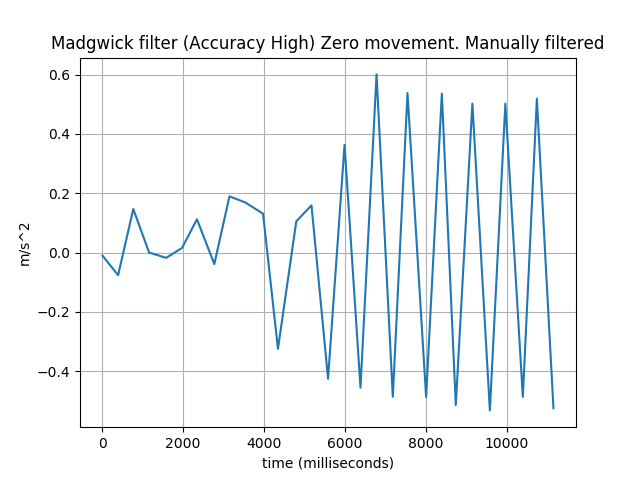
\includegraphics[scale=0.5]{imagenes/madwickZero.png}
	\caption{Compensación de la gravedad por medio del algoritmo de Madgwick (sin movimiento).}
	\label{Movimiento cero Madgwick}
\end{figure}


\begin{figure}[H]
	\centering
	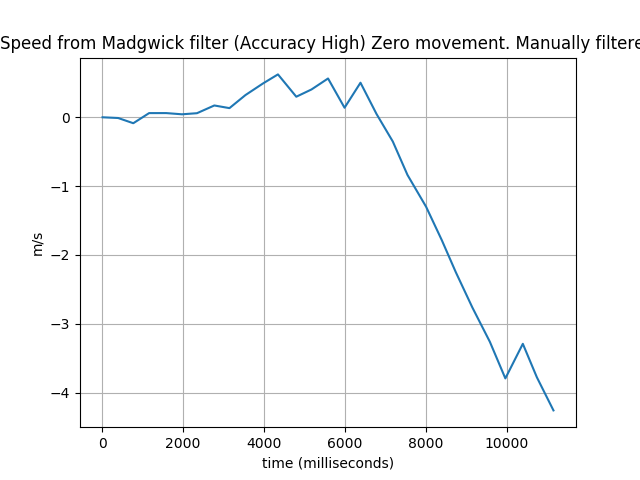
\includegraphics[scale=0.5]{imagenes/madwickZeroSpeed.png}
	\caption{Velocidad calculada de la aceleración por medio del algoritmo de Madgwick (sin movimiento).}
	\label{Velocidad cero Madgwick}
\end{figure}
\noindent
Como se puede ver, la aceleración varía rápidamente y su amplitud va aumentando segundo a segundo, lejos de ser estable y precisa.

\subsubsection{Validación filtro de paso bajo}

\begin{figure}[H]
	\centering
	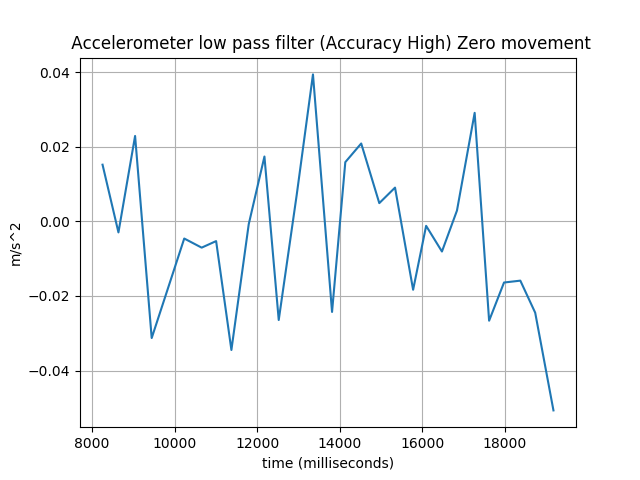
\includegraphics[scale=0.5]{imagenes/lowpass0mov.png}
	\caption{Compensación de la gravedad por medio de un filtro de paso bajo (sin movimiento).}
	\label{Movimiento cero filtro paso bajo}
\end{figure}

\begin{figure}[H]
	\centering
	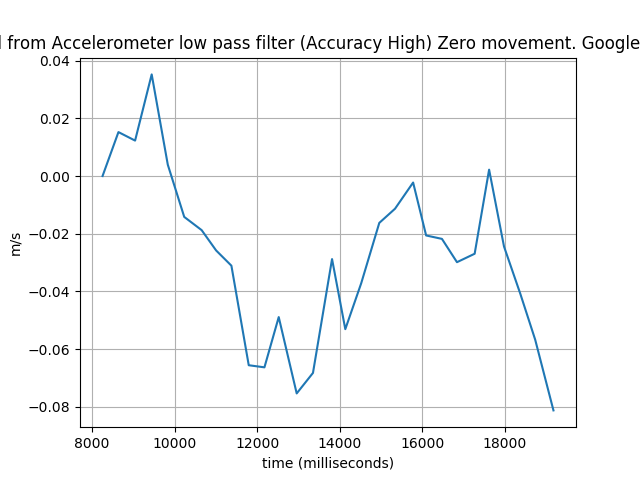
\includegraphics[scale=0.5]{imagenes/lowpass0movspeed.png}
	\caption{Velocidad calculada de la aceleración por medio de un filtro de paso bajo (sin movimiento).}
	\label{Velocidad cero filtro paso bajo}
\end{figure}
\noindent
Se puede observar como la aceleración varía de considerablemente menos que en el método anterior, teniendo una reducción de un -93,33\% en el valor máximo. Donde la diferencia es más notoria es en el cálculo de la velocidad, habiendo una diferencia a los 11000 ms de 4 m/s\^2 a -0,02 m/s\^2.


\subsubsection{Validación aceleración lineal}

\begin{figure}[H]
	\centering
	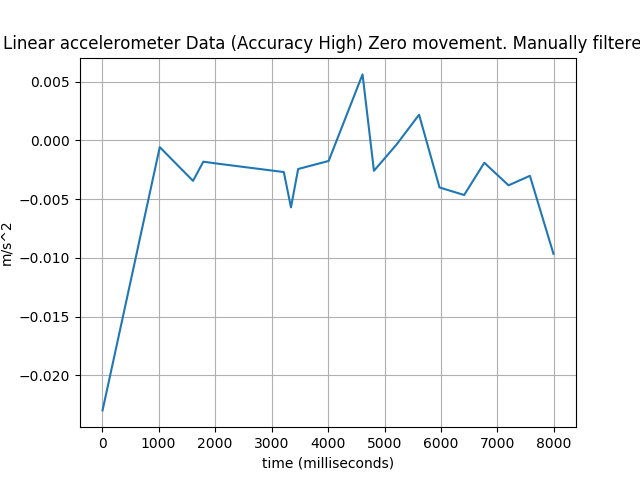
\includegraphics[scale=0.5]{imagenes/linearGoogleZero.png}
	\caption{Compensación de la gravedad por medio de la aceleración lineal (API) (sin movimiento).}
	\label{Movimiento cero aceleracion lineal}
\end{figure}

\begin{figure}[H]
	\centering
	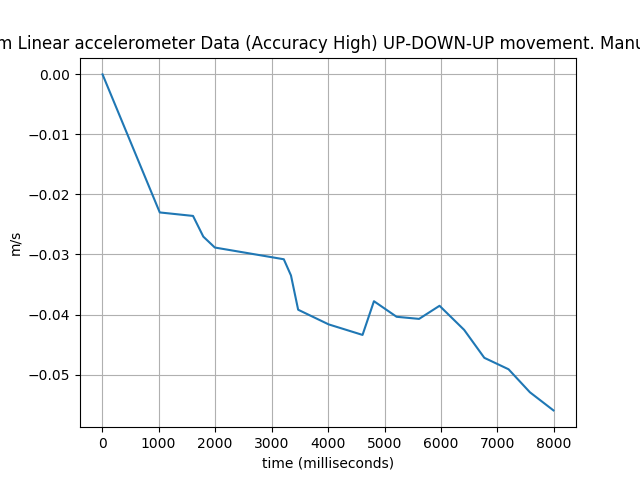
\includegraphics[scale=0.5]{imagenes/linearGoogleZeroSpeed.png}
	\caption{Velocidad calculada de la aceleración lineal (API) (sin movimiento).}
	\label{Velocidad cero aceleracion lineal}
\end{figure}
\noindent
En este caso, se aprecia como la aceleración máxima varía en un -82,61\% con respecto al filtro de paso bajo.
\\
\\
Su funcionamiento en líneas generales es muy parecido al del filtro de paso bajo.

\subsection{Condición de movimiento}

Esta vez se realizarán las pruebas en base al siguiente escenario. Circunstancia de movimiento de 60 cm en total a lo largo del eje Y (+30 cm y -30cm) del wearable y 30 segundos de tiempo de muestreo. Quedando el wearable apoyado sobre una superficie plana al final de la medición. Se debe tener en cuenta que la aceleración máxima producida es de 0,15m/s\^2.\\\\ Tomamos muestras para cada método:

\subsubsection{Validación compensación gravitatoria utilizando Sensor Fusion}

\begin{figure}[H]
	\centering
	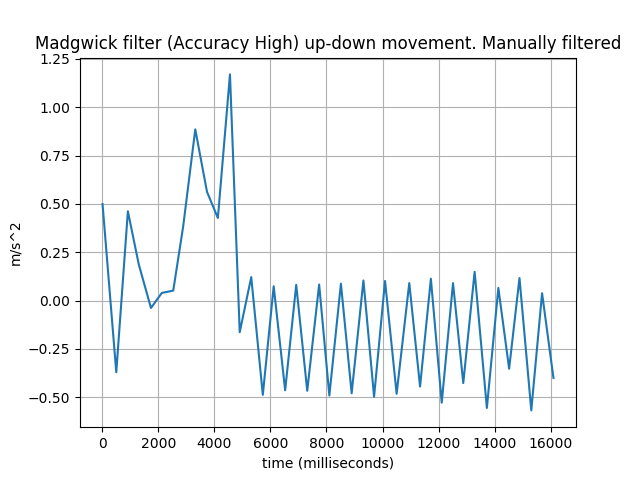
\includegraphics[scale=0.5]{imagenes/madwickup-down.png}
	\caption{Compensación de la gravedad por medio del algoritmo de Madgwick (con movimiento vertical).}
	\label{Movimiento vertical Madgwick}
\end{figure}


\begin{figure}[H]
	\centering
	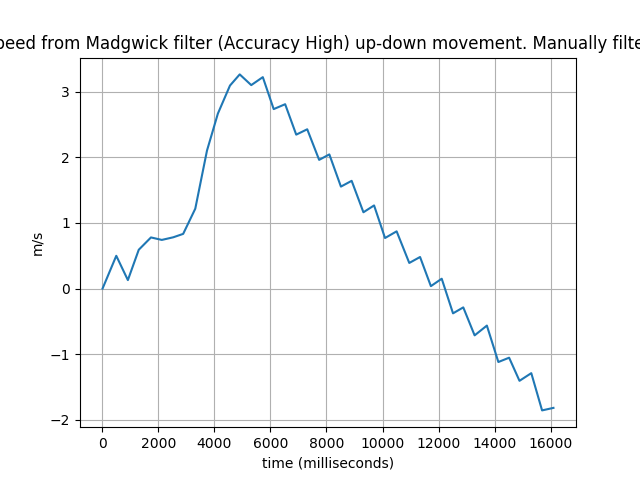
\includegraphics[scale=0.5]{imagenes/madwickup-downSpeed.png}
	\caption{Velocidad calculada de la aceleración por medio del algoritmo de Madgwick (con movimiento vertical).}
	\label{Velocidad vertical Madgwick}
\end{figure}
\noindent
Como se puede apreciar, la aceleración no es nada estable, sobre todo cuando se encuentra en condición de parada. Aumentando la amplitud de la señal en función del tiempo.

\subsubsection{Validación filtro de paso bajo}

\begin{figure}[H]
	\centering
	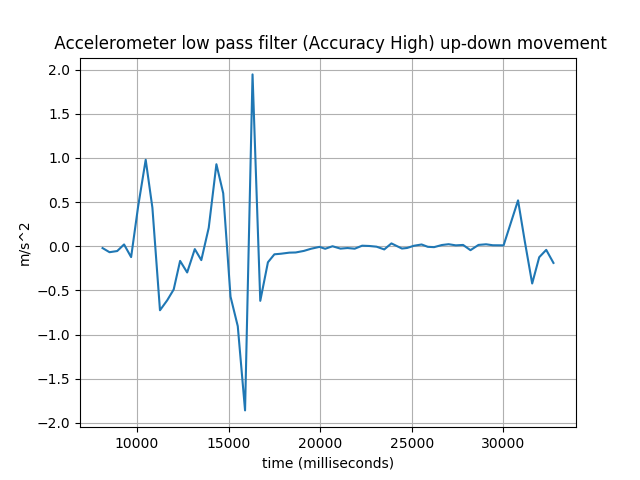
\includegraphics[scale=0.5]{imagenes/lowpassUpmov.png}
	\caption{Compensación de la gravedad por medio de un filtro de paso bajo (con movimiento vertical).}
	\label{Movimiento vertical filtro paso bajo}
\end{figure}

\begin{figure}[H]
	\centering
	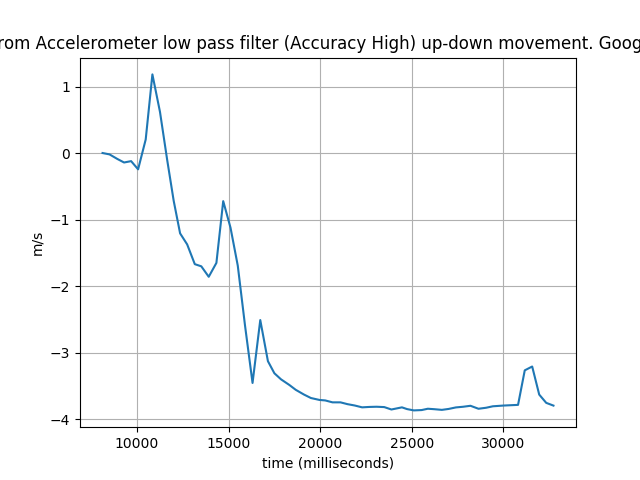
\includegraphics[scale=0.5]{imagenes/lowpassUpmovspeed.png}
	\caption{Velocidad calculada de la aceleración por medio de un filtro de paso bajo (con movimiento vertical).}
	\label{Velocidad vertical filtro paso bajo}
\end{figure}
\noindent
Se puede ver como la aceleración esta vez no flúctua cuando se encuentra en condición de parada, monitorizando correctamente cuando se encuentra en movimiento el dispositivo. Sin embargo, se aprecia como la aceleración en movimiento alcanza valores sustancialmente elevados y altos, no ajustados a la aceleración real.


\subsubsection{Validación aceleración lineal}

\begin{figure}[H]
	\centering
	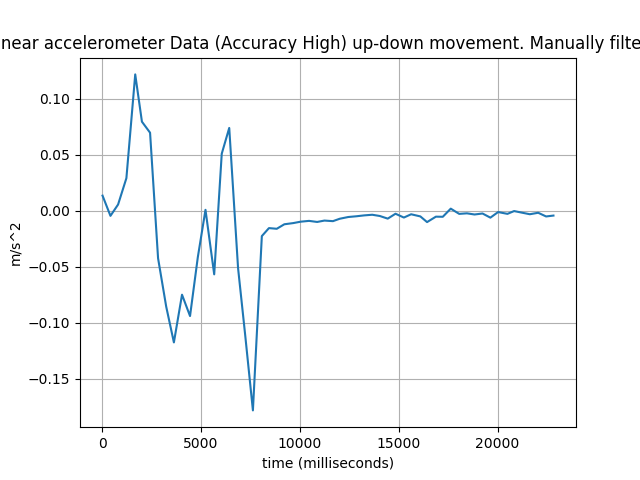
\includegraphics[scale=0.5]{imagenes/linearGoogleup-down.png}
	\caption{Compensación de la gravedad por medio de la aceleración lineal (API) (con movimiento vertical).}
	\label{Movimiento vertical aceleracion lineal}
\end{figure}

\begin{figure}[H]
	\centering
	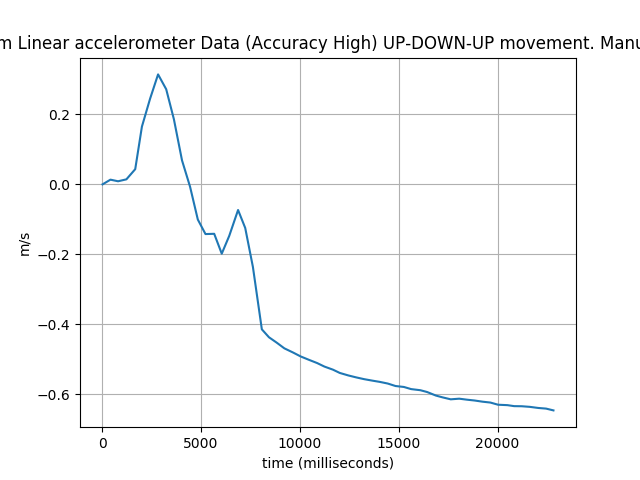
\includegraphics[scale=0.5]{imagenes/linearGoogleup-downSpeed.png}
	\caption{Velocidad calculada de la aceleración lineal (API) (con movimiento vertical).}
	\label{Velocidad vertical aceleracion lineal}
\end{figure}
\noindent
En este caso, la aceleración sí varía entre unos baremos reales, ajustándose más a los valores reales que el resto de métodos. Por lo que a priori parece el método más adecuado para utilizar en el sistema.

\section{Eliminación de ruido mecánico}

Una vez se ha eliminado la componente gravitatoria de los datos, aún cuando el wearable se encuentra en condición de parada, el acelerómetro produce valores inestables.
\\
\\
Por lo que es necesario construir una ventana de discriminación con el fin de considerar los valores que son ruido y los valores que representan aceleración real. De esta manera se mejora la precisión de la aceleración y consecuentemente de la velocidad calculada.
\\
\begin{figure}[H]
	\centering
	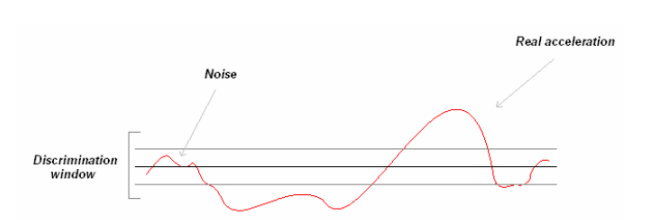
\includegraphics[scale=0.5]{imagenes/ventana.png}
	\caption{Ventana de discriminación \cite{nxp}.}
	\label{Ventana de discriminación}
\end{figure}

%
\chapter{Diseño}

En este capítulo se va a tratar el diseño del sistema. Encontrando 5 secciones. La primera, Diseño del sistema 6.1, describe la arquitectura general del sistema. La segunda, Diagrama de clases de la aplicación móvil 6.2, describe atributos,los principales métodos y relaciones de la aplicación móvil. La tercera, Diagrama de clases de la aplicación wear 6.3, describe atributos, métodos y relaciones de la aplicación wear. La cuarta sección denominada Casos de uso 6.4, contiene los distintos casos de uso de los usuarios en el sistema. Finalmente, la sección Diseño de la base de datos 6.5, describe la estructura de la base de datos.

\section{Diseño del sistema}

Se pueden diferenciar tres partes principales que interactúan entre ellas. La primera una aplicación Android para el dispositivo wearable que será la encargada de recopilar información y enviarla, la segunda, una aplicación Android móvil la cual recibirá los datos, los procesará y los representará visualmente. La tercera parte formada por un servidor(Firebase), será la encargada de almacenar los datos del usuario y los datos que cree.\\
\\
Así que la estructura del proyecto del cual trata este trabajo,  seguirá el siguiente diseño:

\begin{figure}[H]
	\centering
	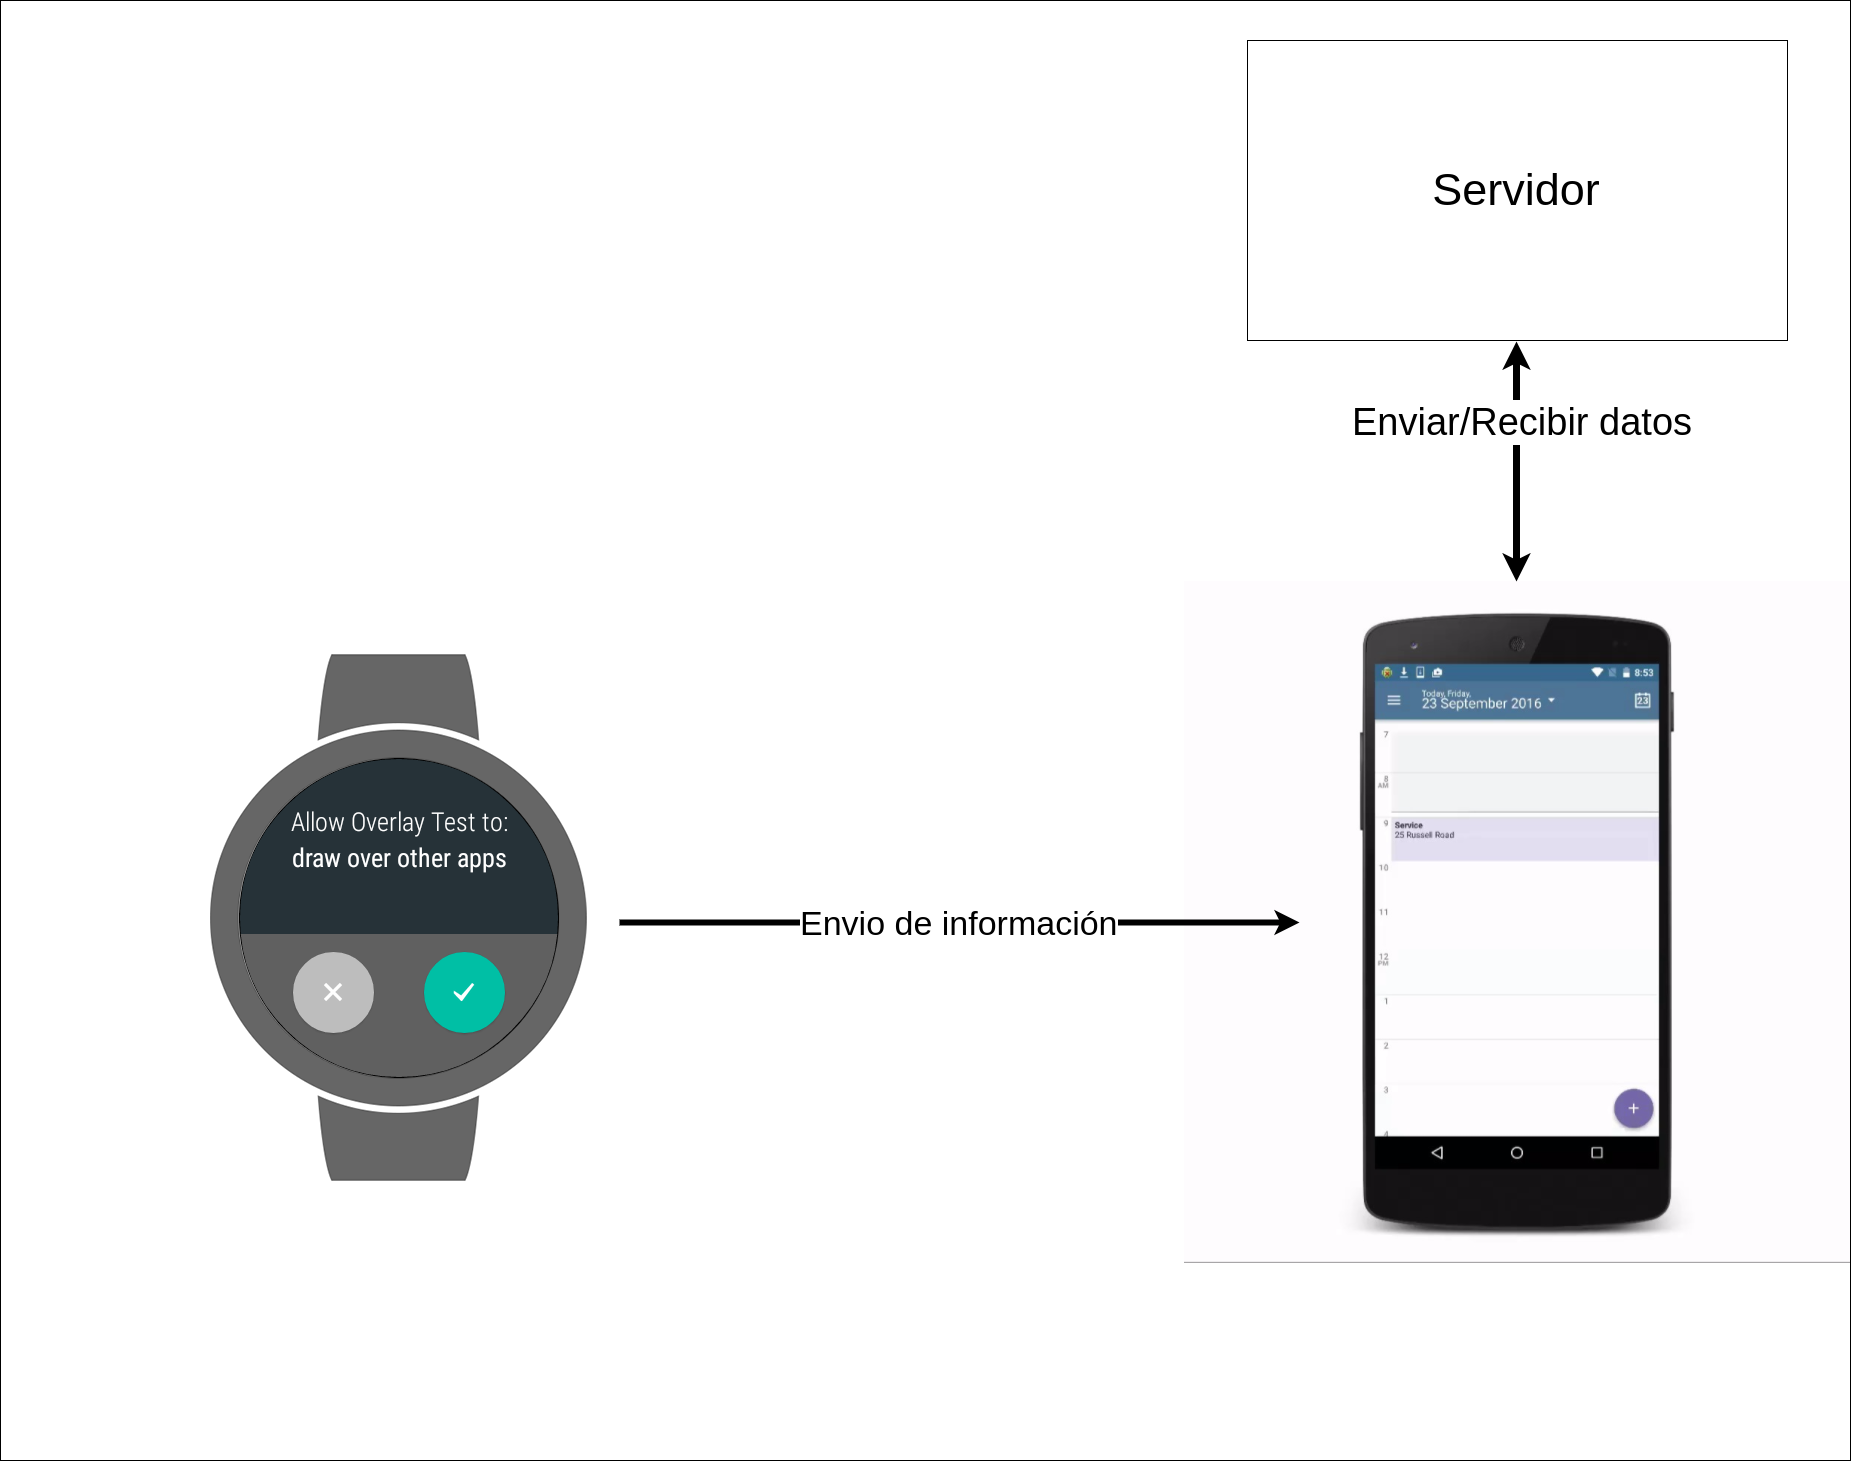
\includegraphics[scale=0.2]{imagenes/disa.png}
	\caption{Arquitectura del proyecto.}
	\label{Arquitectura del proyecto}
\end{figure}
\noindent
En las siguientes secciones de este capítulo se tratará el diseño de cada uno de los componentes de la figura anterior.

\section{Diagrama de clases aplicación móvil}

Esta herramienta describe de manera gráfica utilizando el lenguaje UML las clases y sus relaciones dentro de la aplicación. Otorgando al sistema de todas sus funcionalidades.

\begin{figure}[H]
	\centering
	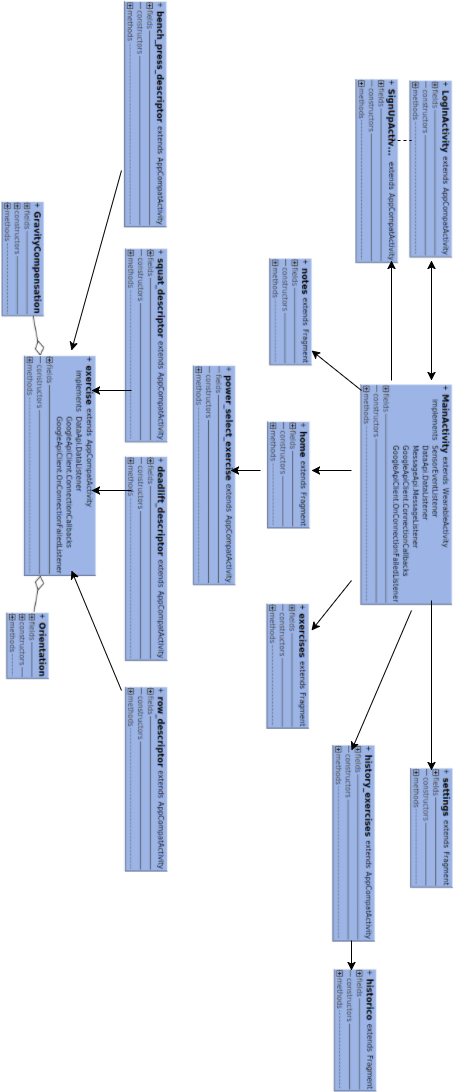
\includegraphics[scale=0.60]{imagenes/clases.jpg}
	\caption{Diagrama de clases de la aplicación móvil.}
	\label{Diagrama de clases android}
\end{figure}

\section{Diagrama de clases aplicación wear}

La finalidad de la aplicación wear es la de recoger y enviar la información, por lo que se ha decidido implementar toda su funcionalidad en una sola clase:

\begin{figure}[H]
	\centering
	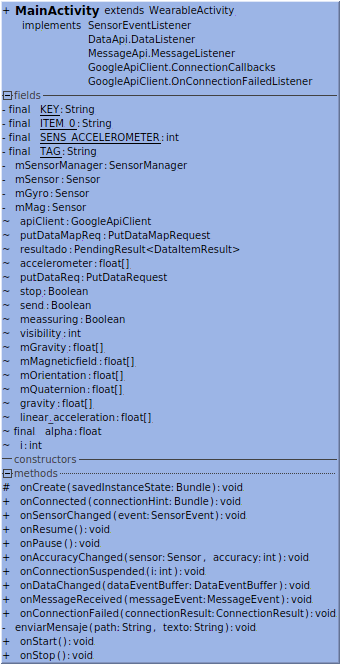
\includegraphics[scale=0.7]{imagenes/clasesW.png}
	\caption{Diagrama de clases de la aplicación wear.}
	\label{Diagrama de clases wear}
\end{figure}

\section{Casos de uso}

En esta sección se va a detallar los casos de uso de la aplicación, los cuales encajan con los requisitos funcionales descritos en el capítulo 3 de este trabajo.\\
\\

\begin{figure}[H]
	\centering
	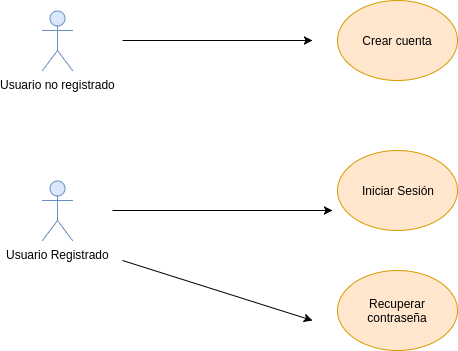
\includegraphics[scale=0.5]{imagenes/uso1.png}
	\caption{Caso de uso 1 - Credenciales.}
	\label{Caso de uso 1}
\end{figure}

\textbf{Crear cuenta}

\begin{table}[h!]
\centering
\caption{Caso de uso - Crear cuenta}
\label{caso de uso crear-cuenta}
\begin{tabular}{|l|l|}
\hline
Titulo         & Crear cuenta                                                                                                                                                                    \\ \hline
Descipción     & \begin{tabular}[c]{@{}l@{}}El usuario puede crearse una cuenta en la aplicación introduciendo \\ el email y una contraseña.\end{tabular}                                        \\ \hline
Actor          & Usuario no registrado                                                                                                                                                           \\ \hline
Precondición   & Que el email no se encuentre ya en el sistema                                                                                                                                   \\ \hline
Secuencia      & \begin{tabular}[c]{@{}l@{}}- El usuario instala la aplicación.\\  - El usuario entra en la aplicación.\\  - Introducir los campos\\  - Pulsar el botón de registro\end{tabular} \\ \hline
Post condición & El usuario entra en la aplicación y ya dispone de credenciales                                                                                                                  \\ \hline
Comentarios    & \begin{tabular}[c]{@{}l@{}}El campo email debe ser un email válido y accesible, pues se \\ utilizará para restaurar la contraseña.\end{tabular}                                 \\ \hline
\end{tabular}
\end{table}

\textbf{Iniciar sesión}
\begin{table}[H]
\centering
\caption{Caso de uso - Inicio sesión}
\label{caso de uso inicio-sesion}
\begin{tabular}{|l|l|}
\hline
Titulo         & Iniciar sesión                                                                                                                                  \\ \hline
Descipción     & \begin{tabular}[c]{@{}l@{}}El usuario podrá iniciar sesión utilizando los credenciales que \\  creó previamente.\end{tabular}                 \\ \hline
Actor          & Usuario registrado                                                                                                                           \\ \hline
Precondición   & Que el usuario se encuentre registrado en el sistema                                                                                            \\ \hline
Secuencia      & \begin{tabular}[c]{@{}l@{}}- El usuario entra en la aplicación\\  - Introducir los campos\\  - Pulsar el botón de inicio de sesión\end{tabular} \\ \hline
Post condición & El usuario se encuentra dentro de la aplicación                                                                                                 \\ \hline
Comentarios    & El usuario debe memorizar su email y contraseña.                                                                                                \\ \hline
\end{tabular}
\end{table}

\textbf{Recuperar contraseña}
\begin{table}[H]
\centering
\caption{Caso de uso - Recuperar contraseña}
\label{caso de uso recuperar-contraseña}
\begin{tabular}{|l|l|}
\hline
Titulo         & Recuperar Contraseña                                                                                                                                 \\ \hline
Descipción     & \begin{tabular}[c]{@{}l@{}}El usuario podrá recupera la contraseña utilizando los credenciales que \\  creó previamente (email).\end{tabular}                 \\ \hline
Actor          & Usuario registrado                                                                                                                           \\ \hline
Precondición   & Que el usuario se encuentre registrado en el sistema                                                                                            \\ \hline
Secuencia      & \begin{tabular}[c]{@{}l@{}}- El usuario entra en la aplicación\\  - Introduce el campo email\\  - Pulsar el botón de recuperar contraseña \\ Accede a su email y recupera la contraseña\end{tabular} \\ \hline
Post condición & El usuario obtiene su contraseña                                                                                                 \\ \hline
Comentarios    & El usuario debe memorizar su email y contraseña.                                                                                                \\ \hline
\end{tabular}
\end{table}

\begin{figure}[H]
	\centering
	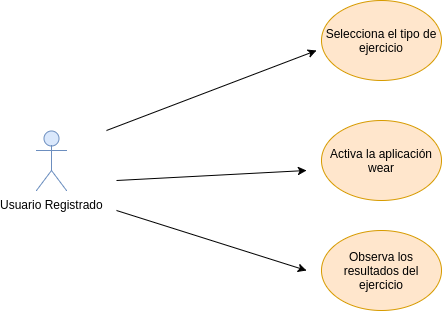
\includegraphics[scale=0.5]{imagenes/uso2.png}
	\caption{Caso de uso 2 - Realización del ejercicio.}
	\label{Caso de uso 2}
\end{figure}

\textbf{Selección del tipo de ejercicio}

\begin{table}[H]
\centering
\caption{Caso de uso - Seleccionar ejercicio}
\label{Caso de uso - Seleccionar ejercicio}
\begin{tabular}{|l|l|}
\hline
Titulo         & Selección del tipo de ejercicio                                                                                                                            \\ \hline
Descipción     & \begin{tabular}[c]{@{}l@{}}El usuario podrá seleccionar el tipo de ejercicio\\ que va a realizar.\end{tabular}                                             \\ \hline
Actor          & Usuario registrado                                                                                                                                         \\ \hline
Precondición   & Que el usuario se encuentre registrado en el sistema                                                                                                       \\ \hline
Secuencia      & \begin{tabular}[c]{@{}l@{}}- El usuario entra en la aplicación\\ - Pulsar la pestaña de ejercicio\\ - Selecciona el tipo de ejercicio deseado\end{tabular} \\ \hline
Post condición & El usuario se encuentra con la descripción del ejercicio                                                                                                   \\ \hline
Comentarios    & \begin{tabular}[c]{@{}l@{}}El usuario debe leer la descripción para realizar el\\ ejercicio correctamente y de manera segura\end{tabular}                  \\ \hline
\end{tabular}
\end{table}

\textbf{Inicio de la monitorización del ejercicio}
\begin{table}[H]
\centering
\caption{Caso de uso - Inicio de la monitorización del ejercicio}
\label{Caso de uso - Inicio de la monitorización del ejercicio}
\begin{tabular}{|l|l|}
\hline
Titulo         & Activar la monitorización de la aplicación wear                                                                                                                                                                              \\ \hline
Descipción     & \begin{tabular}[c]{@{}l@{}}El usuario podrá indicar cuando va a comenzar el \\ ejercicio.\end{tabular}                                                                                                                       \\ \hline
Actor          & Usuario registrado                                                                                                                                                                                                           \\ \hline
Precondición   & \begin{tabular}[c]{@{}l@{}}Que el usuario se encuentre registrado en el sistema y \\ haya seleccionado un ejercicio.\end{tabular}                                                                                            \\ \hline
Secuencia      & \begin{tabular}[c]{@{}l@{}}- El usuario entra en la aplicación\\ - Pulsar la pestaña de ejercicio\\ - Selecciona el tipo de ejercicio deseado\\ - Inicia la aplicación wear.\\ - Selecciona el botón de inicio.\end{tabular} \\ \hline
Post condición & El usuario se encuentra realizando el ejercicio                                                                                                                                                                              \\ \hline
Comentarios    & \begin{tabular}[c]{@{}l@{}}El usuario debe leer la descripción para realizar el\\ ejercicio correctamente y de manera segura\end{tabular}                                                                                    \\ \hline
\end{tabular}
\end{table}

\textbf{Visualización de los resultados}
\begin{table}[H]
\centering
\caption{Caso de uso - Visualización de los resultados }
\label{Visualización de los resultados }
\begin{tabular}{|l|l|}
\hline
Titulo         & Visualización de los resultados                                                                                                                                                                                                                                                           \\ \hline
Descipción     & \begin{tabular}[c]{@{}l@{}}El usuario podrá visualizar la potencia realizada\\ en tiempo real.\end{tabular}                                                                                                                                                                               \\ \hline
Actor          & Usuario registrado                                                                                                                                                                                                                                                                        \\ \hline
Precondición   & \begin{tabular}[c]{@{}l@{}}Que el usuario se encuentre registrado en el sistema, \\ haya seleccionado un ejercicio y haya activado la\\ aplicación wear.\end{tabular}                                                                                                                     \\ \hline
Secuencia      & \begin{tabular}[c]{@{}l@{}}- El usuario entra en la aplicación\\ - Pulsar la pestaña de ejercicio\\ - Selecciona el tipo de ejercicio deseado\\ - Inicia la aplicación wear.\\ - Selecciona el botón de inicio.\\ - Observa como se procesa la información en tiempo\\ real.\end{tabular} \\ \hline
Post condición & El usuario termina la serie.                                                                                                                                                                                                                                                              \\ \hline
Comentarios    & \begin{tabular}[c]{@{}l@{}}El usuario debe leer la descripción para realizar el\\ ejercicio correctamente y de manera segura\end{tabular}                                                                                                                                                 \\ \hline
\end{tabular}
\end{table}


\begin{figure}[H]
	\centering
	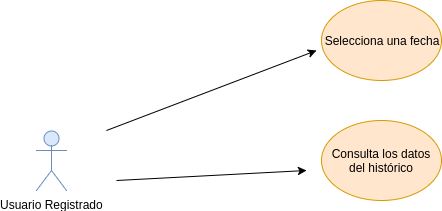
\includegraphics[scale=0.5]{imagenes/uso3.png}
	\caption{Caso de uso 3 - Consulta del histórico.}
	\label{Caso de uso 3}
\end{figure}

\textbf{Selección de una fecha}
\begin{table}[H]
\centering
\caption{Caso de uso - Selección de una fecha}
\label{Caso de uso -  Selección de una fecha}
\begin{tabular}{|l|l|}
\hline
Titulo         & Selección de una fecha                                                                                                                                 \\ \hline
Descipción     & \begin{tabular}[c]{@{}l@{}}El usuario podrá seleccionar una fecha para realizar \\ una consulta.\end{tabular}                                          \\ \hline
Actor          & Usuario registrado                                                                                                                                     \\ \hline
Precondición   & Que el usuario se encuentre registrado en el sistema.                                                                                                  \\ \hline
Secuencia      & \begin{tabular}[c]{@{}l@{}}- El usuario entra en la aplicación\\ - Pulsar la pestaña de historico\\ - Selecciona una fecha del calendario\end{tabular} \\ \hline
Post condición & El usuario visualiza los datos para dicha entrada.                                                                                                     \\ \hline
Comentarios    & \begin{tabular}[c]{@{}l@{}}Si el usuario no realizó ninguna actividad durante \\ dicho día no verá información.\end{tabular}                           \\ \hline
\end{tabular}
\end{table}

\textbf{Consulta de los datos del histórico }
\begin{table}[H]
\centering
\caption{Caso de uso - Consulta de los datos del histórico }
\label{Caso de uso - Consulta de los datos del histórico}
\begin{tabular}{|l|l|}
\hline
Titulo         & Consulta de los datos del histórico                                                                                                                                                               \\ \hline
Descipción     & \begin{tabular}[c]{@{}l@{}}El usuario podrá visualizar su entrenamiento de\\ un día dado.\end{tabular}                                                                                            \\ \hline
Actor          & Usuario registrado                                                                                                                                                                                \\ \hline
Precondición   & \begin{tabular}[c]{@{}l@{}}Que el usuario se encuentre registrado en el sistema y \\ haya seleccionado una fecha.\end{tabular}                                                                    \\ \hline
Secuencia      & \begin{tabular}[c]{@{}l@{}}- El usuario entra en la aplicación\\ - Pulsar la pestaña de historico\\ - Selecciona una fecha del calendario\\ -Visualiza sus datos el dia seleccionado\end{tabular} \\ \hline
Post condición & El usuario visualiza los datos para dicha entrada.                                                                                                                                                \\ \hline
Comentarios    & \begin{tabular}[c]{@{}l@{}}Si el usuario no realizó ninguna actividad durante \\ dicho día no verá información.\end{tabular}                                                                      \\ \hline
\end{tabular}
\end{table}

\section{Diseño de la base de datos}

Como se ha comentado en el capítulo 2 de este documento. La base de datos se va a almacenar en Firebase, que utiliza una estructura no-SQL, utilizando un formato JSON, por lo que se ha decidido almacenar la base de datos de la siguiente manera, con el fin de agilizar la escritura/lectura de los datos de una manera rápida:

\begin{table}[H]
\centering
\caption{Estructura de la base de datos}
\label{Estructura de la base de datos}
\begin{tabular}{|llllll|}
\hline
Usuarios : \{ &           &             &                &      &       \\
         & IdUsuario : \{ &             &                &      &       \\
         &           & FechaActual : \{ &                &      &       \\
         &           &             & Tipo ejercicio : \{ &      &       \\
         &           &             &                & Hora : \{ &       \\
         &           &             &                &      & Datos: [] \\
         &           &             &                &      \}&  \\
         &           &             &               \}&      &  \\
         &           &             \}&               &      &  \\
         &           \}&             &               &      &  \\
         \}&           &             &               &      &  \\
\hline
\end{tabular}
\end{table}

%
\chapter{Implementación}

En esta sección vamos a tratar como se ha implementado el proyecto sobre el cual se basa esta memoria y sus principales módulos.Contiene 3 secciones. La primera llamada Hito 1: Asistente entrenamiento potencia 7.1, describe los pasos realizados para implementar el ecosistema de la aplicación móvil. La segunda, denominada Hito 2: Uso del servidor, describe los pasos realizados para implementar la conexión con el servidor. Finalmente, la sección Capturas 7.3, contiene capturas sobre la aplicación.
\\
\\

La arquitectura del proyecto sigue el siguiente esquema, el cual se ha desarrollado a lo largo de las dos historias de usuario:

\begin{figure}[H]
	\centering
	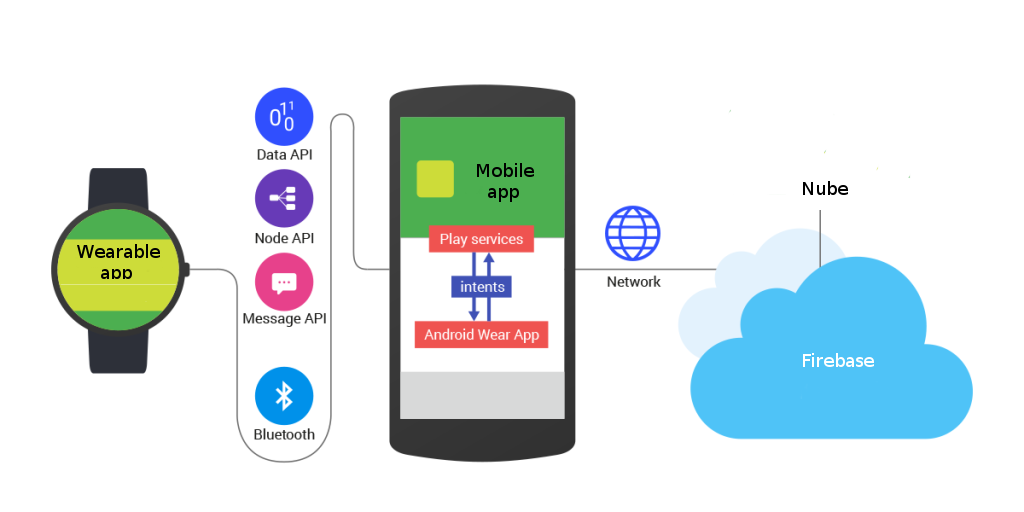
\includegraphics[scale=0.4]{imagenes/arquitectura.png}
	\caption{Diagrama de clases de la aplicación móvil.}
	\label{Arquitectura del sistema}
\end{figure}

El proyecto ha sido desarrollado en Android, por lo que la parte lógica ha sido totalmente programada en Java y utiliza XML para crear las distintas vistas.

\section{Hito 1: Asistente entrenamiento potencia}


El primer paso fue la creación de dos aplicaciones básicas, las cuales incluían una actividad MainActivity, sin ninguna funcionalidad. Una vez creadas ambas aplicaciones había que establecer un cauce de comunicación entre ambas aplicaciones, para ello se ha utilizado la API GoogleApiClient.
\\
Debemos tener en cuenta de que para realizar la conexión, debe haberse instalado previamente la aplicación Android Wear y debe estar enlazada al smartwatch que deseemos usar. Una vez hemos creado una instancia de GoogleApiClient, debemos conectar a la API Wearable API. Se debe establecer la conexión tanto en la aplicación wear como en la móvil para crear el cauce de comunicación.
\\
\\
Tras la creación de un cauce de comunicación entre ambas aplicaciones, se procedió a la obtención de los datos de los sensores. Para ello se utilizo la API de Android y el tipo de sensor TYPE\_LINEAR\_ACCELERATION. Que como se pudo ver en el capítulo 5, fue el método que menor error produjo en las muestras.
\\
\\
De manera paralela, se creó una selección de ejercicios disponibles en la aplicación móvil, añadiendo una pequeña descripción a cada ejercicio.
\\
\\
Una vez obtenidos los datos, se procedió al envío de los mismos en la aplicación Wear, haciendo uso del cauce que se había creado previamente. Utilizando la API DataApi, se creó un objeto DataItem, el cual mediante peticiones se utiliza para el envío de datos sincronizados.\\
A su vez, se procedió a la creación de un listener para el DataItem (utilizando también la API DataApi) en la aplicación móvil, de modo que los datos fueran recibidos en la aplicación móvil.
\\
\\
Todo este proceso se realizó sin ningún control del envio y recepción, siendo estos realizados de manera automática. Por lo que tras estos pasos, se procedió a crear una interfaz de control en la aplicación wear para poder iniciar y detener el envío de información. Dando por finalizada la aplicación Wear.
\\
\\
Estando la comunicación establecida y una vez recibidos los datos se procedió al filtrado de los datos por medio de una ventana de discriminación con el fin de eliminar parte del ruido de los datos.
\\
Posteriormente, con los datos procesados, se procedió al cálculo de la velocidad utilizando un algoritmo de integración. Representando la velocidad calculada haciendo uso de la librería GraphView\cite{graphview}. Cuyo código puede ser consultado en la página del desarrollador y se encuentra bajo licencia Apache v2.
\\
\\
Finalmente, se introdujo un campo para que el usuario introduzca el peso con el que va a realizar el ejercicio y con estos datos, se produjo a calcular la potencia obtenida en cada momento por el usuario.
\\
\\
Estando así la funcionalidad principal de la aplicación completa y totalmente operativa. Sin embargo, carecía de una interfaz gráfica que facilitase la experiencia del usuario. Por lo que se procedió a la creación de un menú  en base a Bottom navigation de material design\cite{navigation}. Utilizando fragments para las distintas vistas del menú.

\section{Hito 2: Uso del servidor}

En este hito se centró en ampliar la funcionalidad de la aplicación por medio de un servidor.
\\
\\
El primer paso fue crear un proyecto en la consola de Firebase.
\\
Una vez importado el paquete Firebase en la aplicación móvil, se utilizó la librería auth para la creación de usuarios (previa activación en la consola de Firebase), inicio de sesión y mantenimiento de la sesión.
\\
Para la obtención de credenciales se crearon dos vistas, una para el registro y otra para el inicio de sesión. En las cuales se obtienen los datos del usuario.
\\
\\
Se utiliza la librería database para las operaciones de escritura lectura de la base de datos, siguiendo el esquema que se diseño en la fase de diseño de la base de datos. Escribiendo en la base de datos al realizar el ejercicio y creando una nueva vista para recuperar los datos guardados en la base de datos, utilizando el criterio de la fecha como clave de búsqueda.
\\
\\
Además, cuando el sistema se encuentre sin conexión a la red y se este realizando un ejercicio. El sistema guardará los datos en almacenamiento local, procediendo al envío de los mismos en cuanto se disponga de conexión y liberando así el espacio ocupado.

\section{Capturas}

Tras la finalización de los dos hitos, a continuación se adjuntan capturas de pantalla de la aplicación.

\subsection*{Android Wear}

En la aplicación de Adroid Wear solo contamos con una vista, la cual va cambiando si el usuario quiere comenzar o terminar un ejercicio.

\begin{figure}[H]
	\centering
	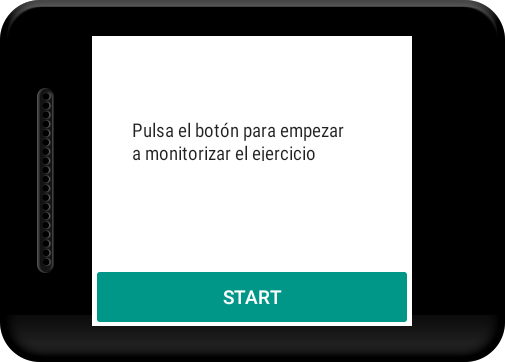
\includegraphics[scale=0.4]{imagenes/w1.png}
	\caption{Pantalla principal Wear}
	\label{Pantalla principal Wear}
\end{figure}

\begin{figure}[H]
	\centering
	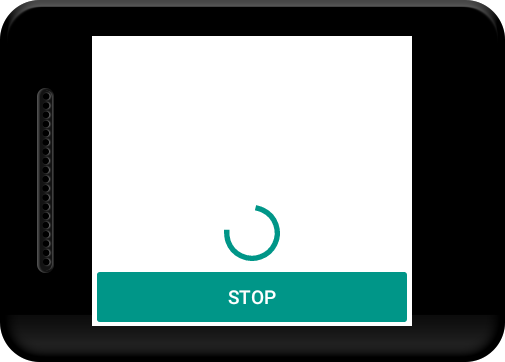
\includegraphics[scale=0.4]{imagenes/w2.png}
	\caption{Realizar medición Wear}
	\label{Realizar medición Wear}
\end{figure}

\subsection*{Android}

Las vistas más importantes de la aplicación móvil son:

\begin{figure}[H]
	\centering
	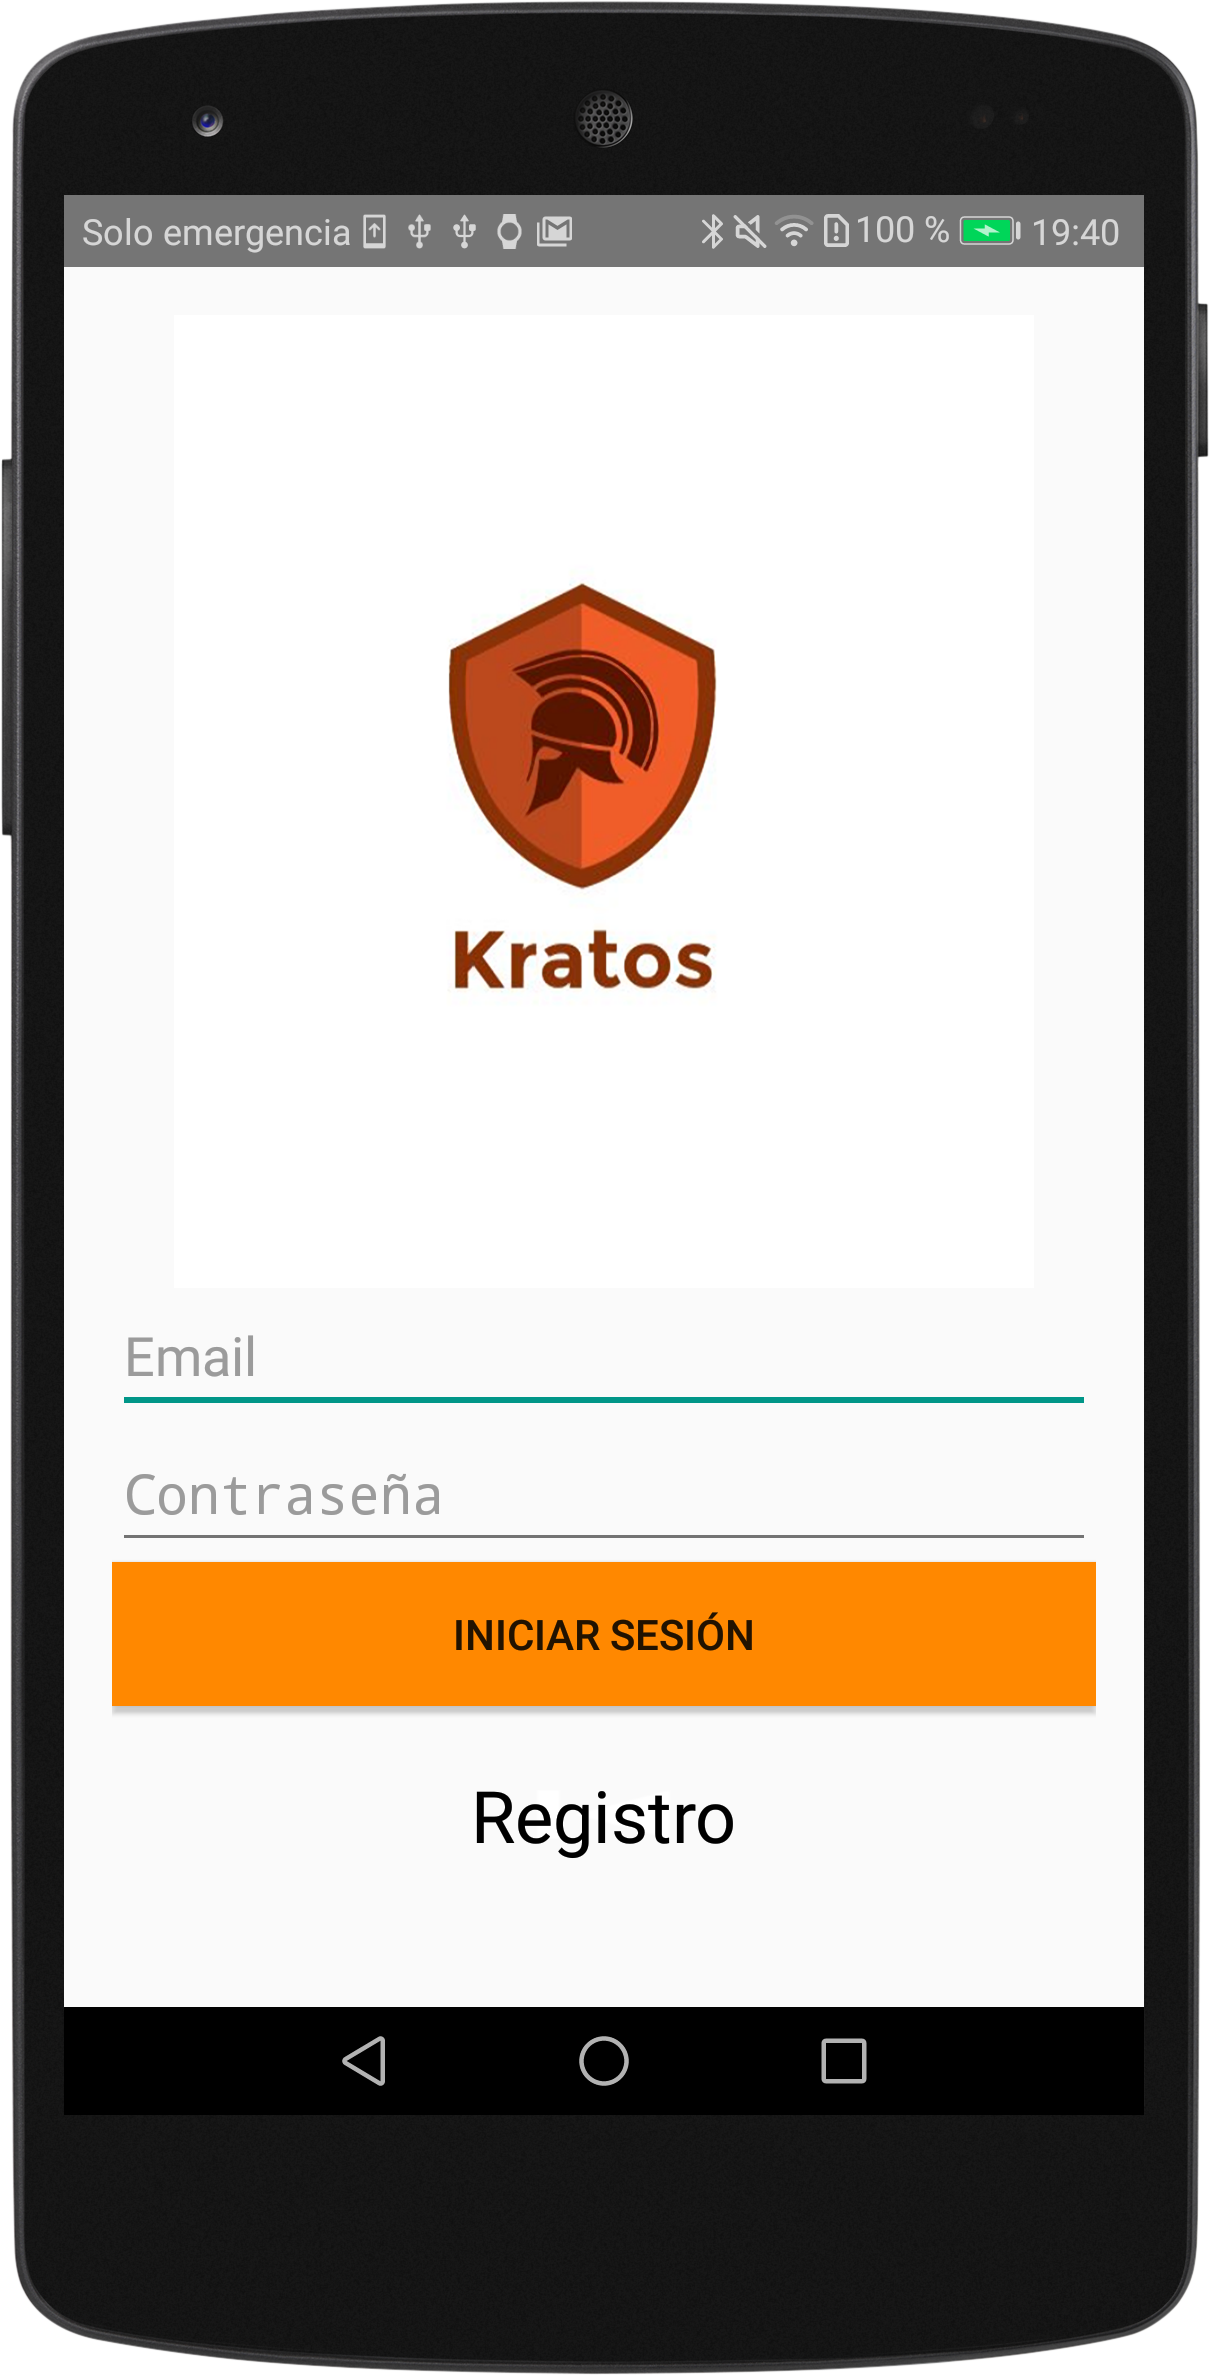
\includegraphics[scale=0.10]{imagenes/m1.png}
	\caption{Pantalla inicio sesión móvil}
	\label{Pantalla inicio sesión móvil}
\end{figure}

\begin{figure}[H]
	\centering
	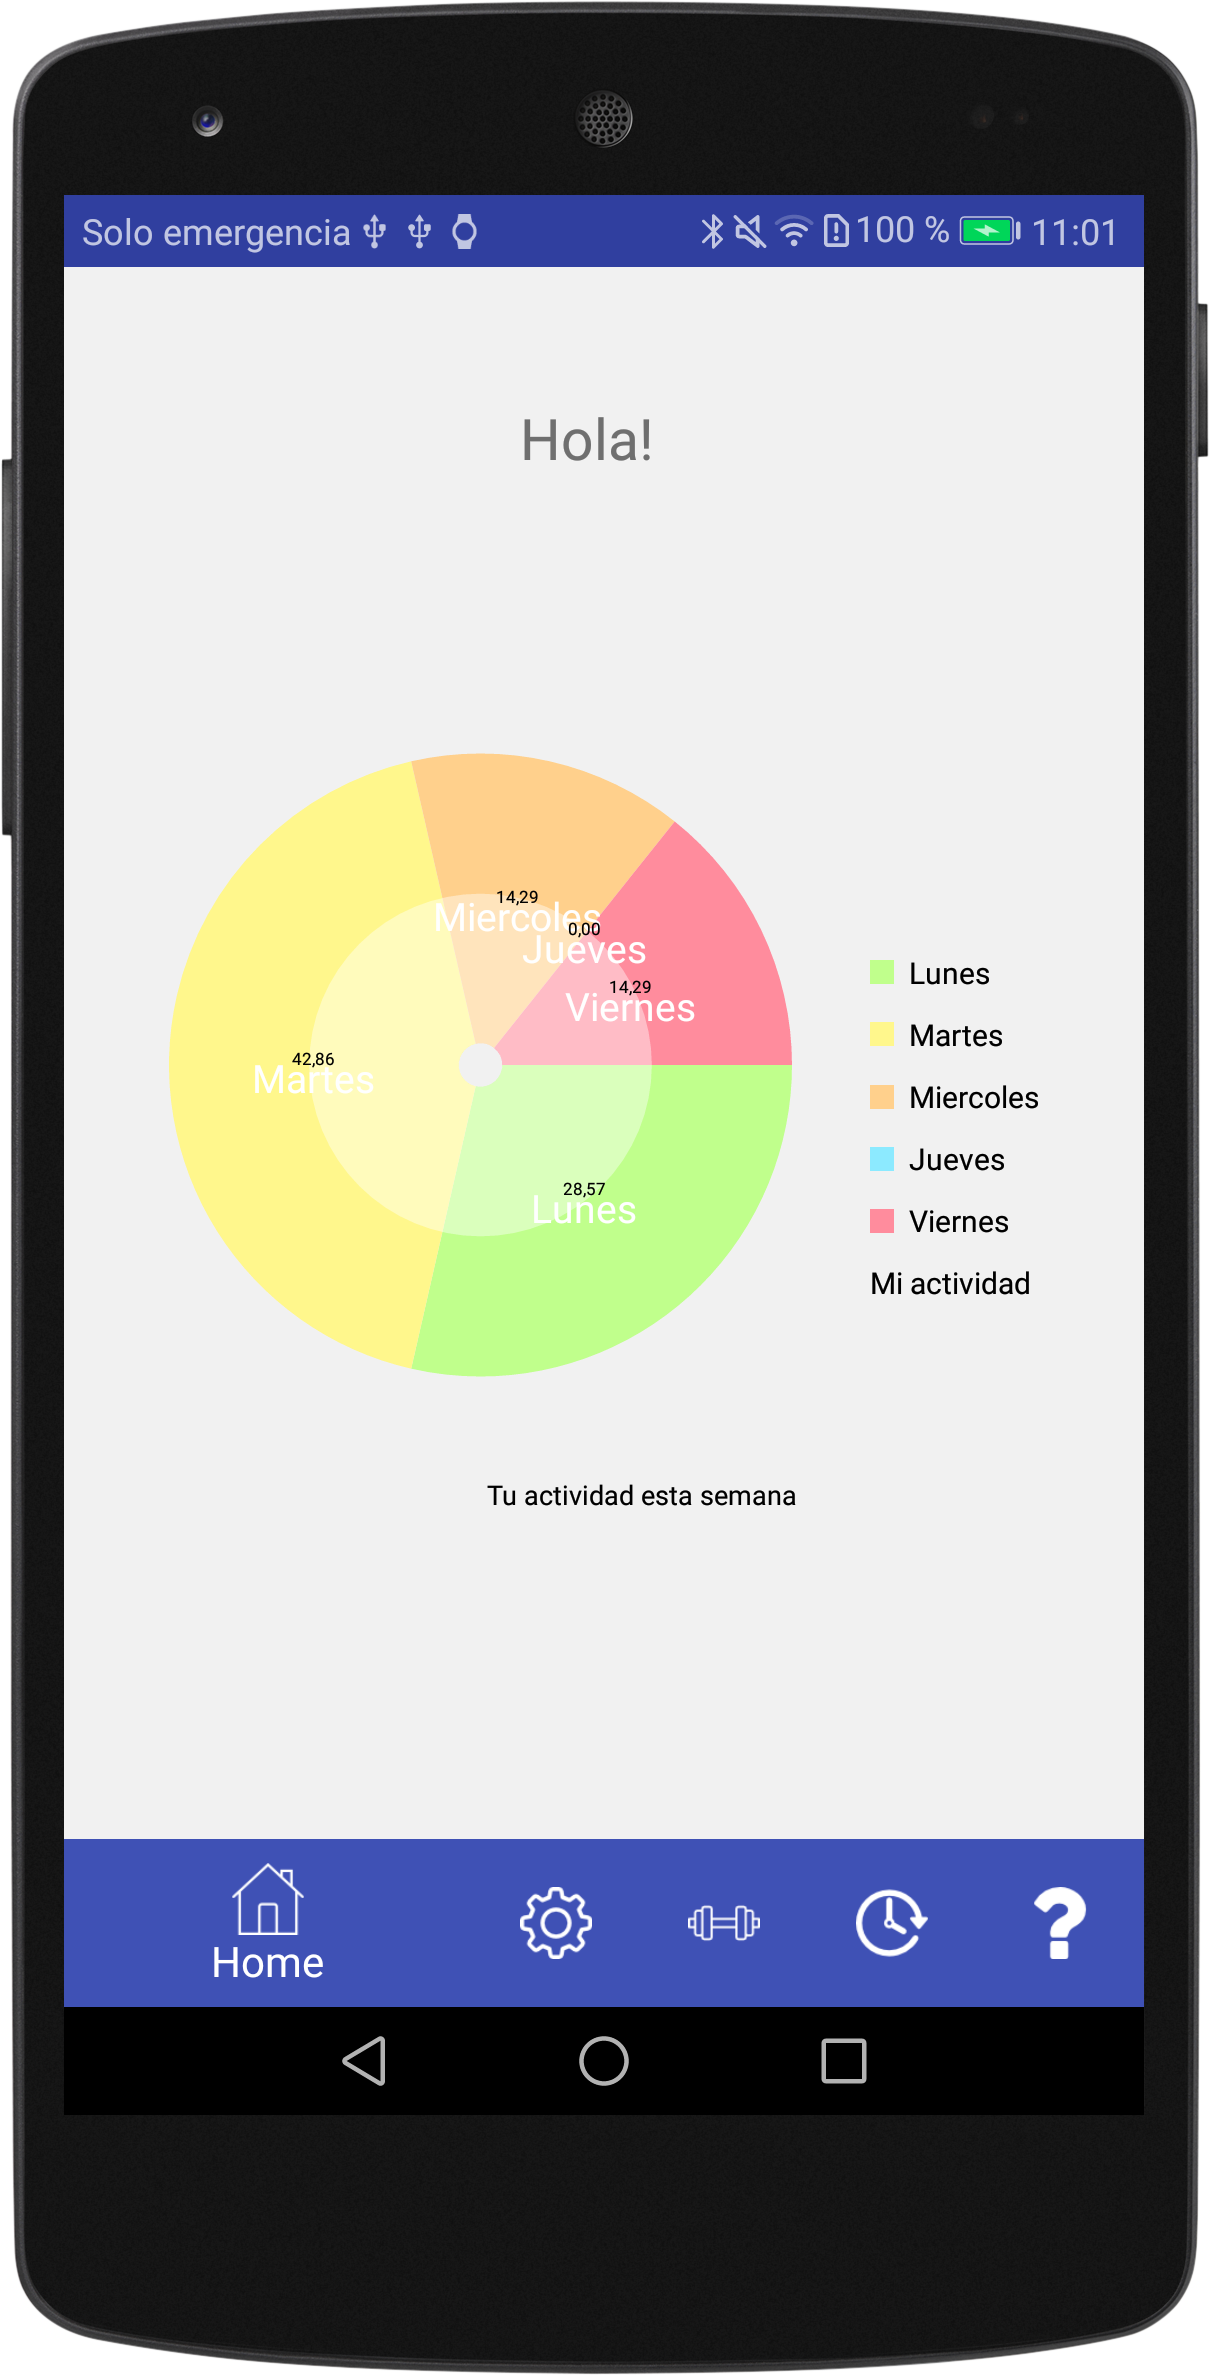
\includegraphics[scale=0.10]{imagenes/m2.png}
	\caption{Pantalla principal móvil}
	\label{Pantalla principal movil}
\end{figure}

\begin{figure}[H]
	\centering
	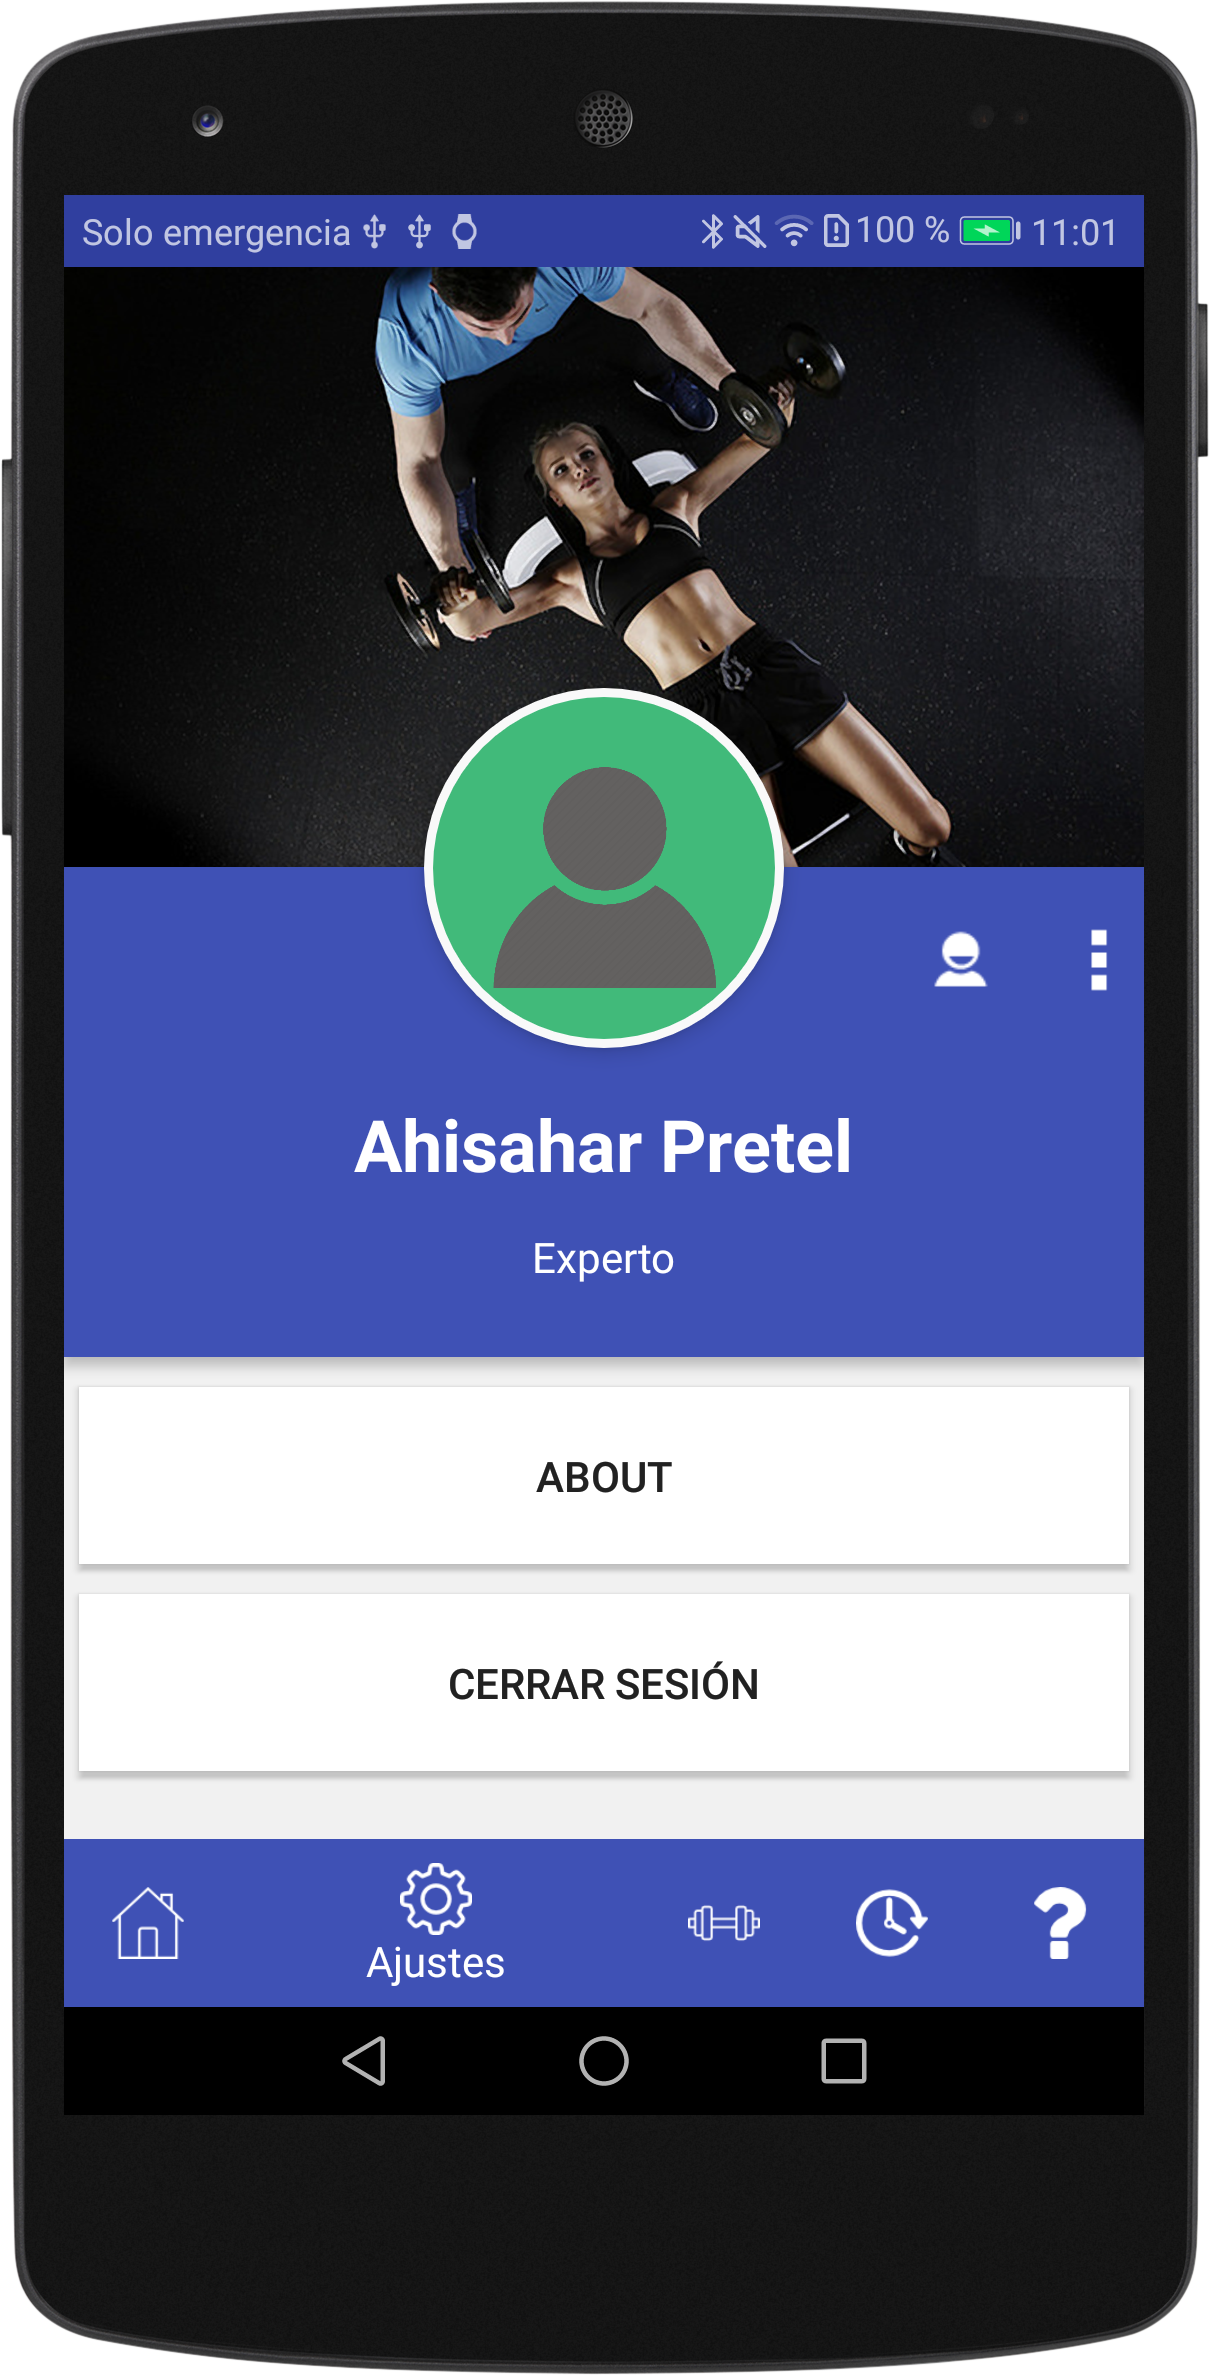
\includegraphics[scale=0.10]{imagenes/m3.png}
	\caption{Vista menú móvil}
	\label{Vista menú movil}
\end{figure}

\begin{figure}[H]
	\centering
	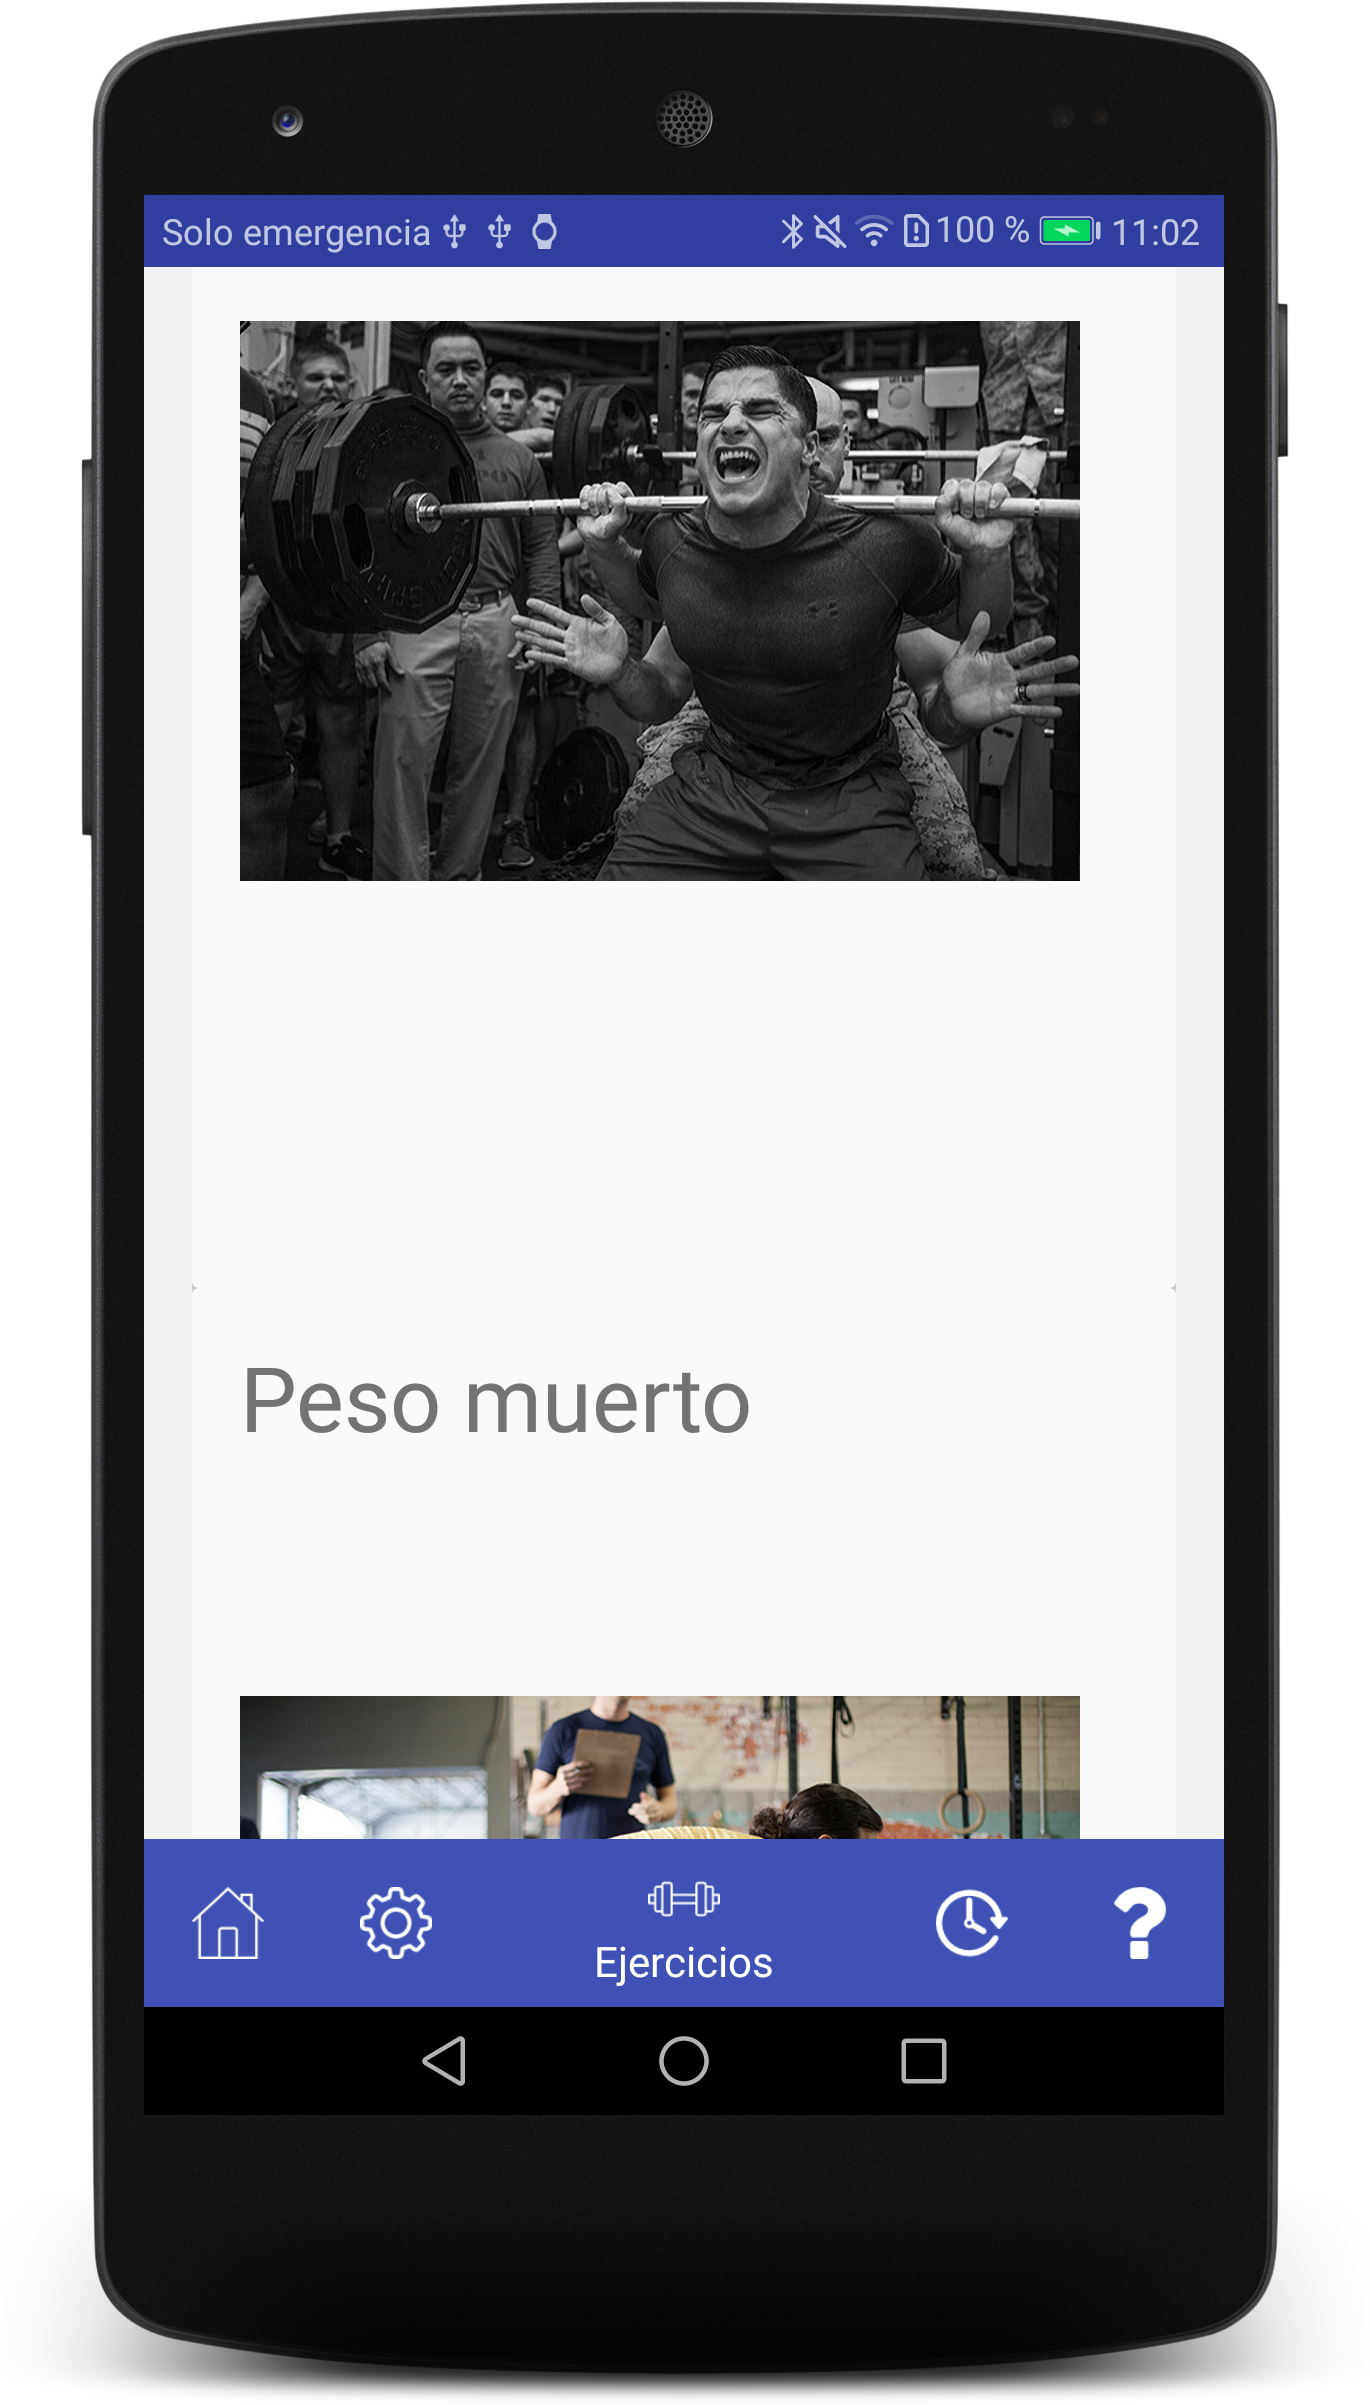
\includegraphics[scale=0.10]{imagenes/m4.png}
	\caption{Vista selección ejercicio móvil}
	\label{Vista selección ejercicio movil}
\end{figure}

\begin{figure}[H]
	\centering
	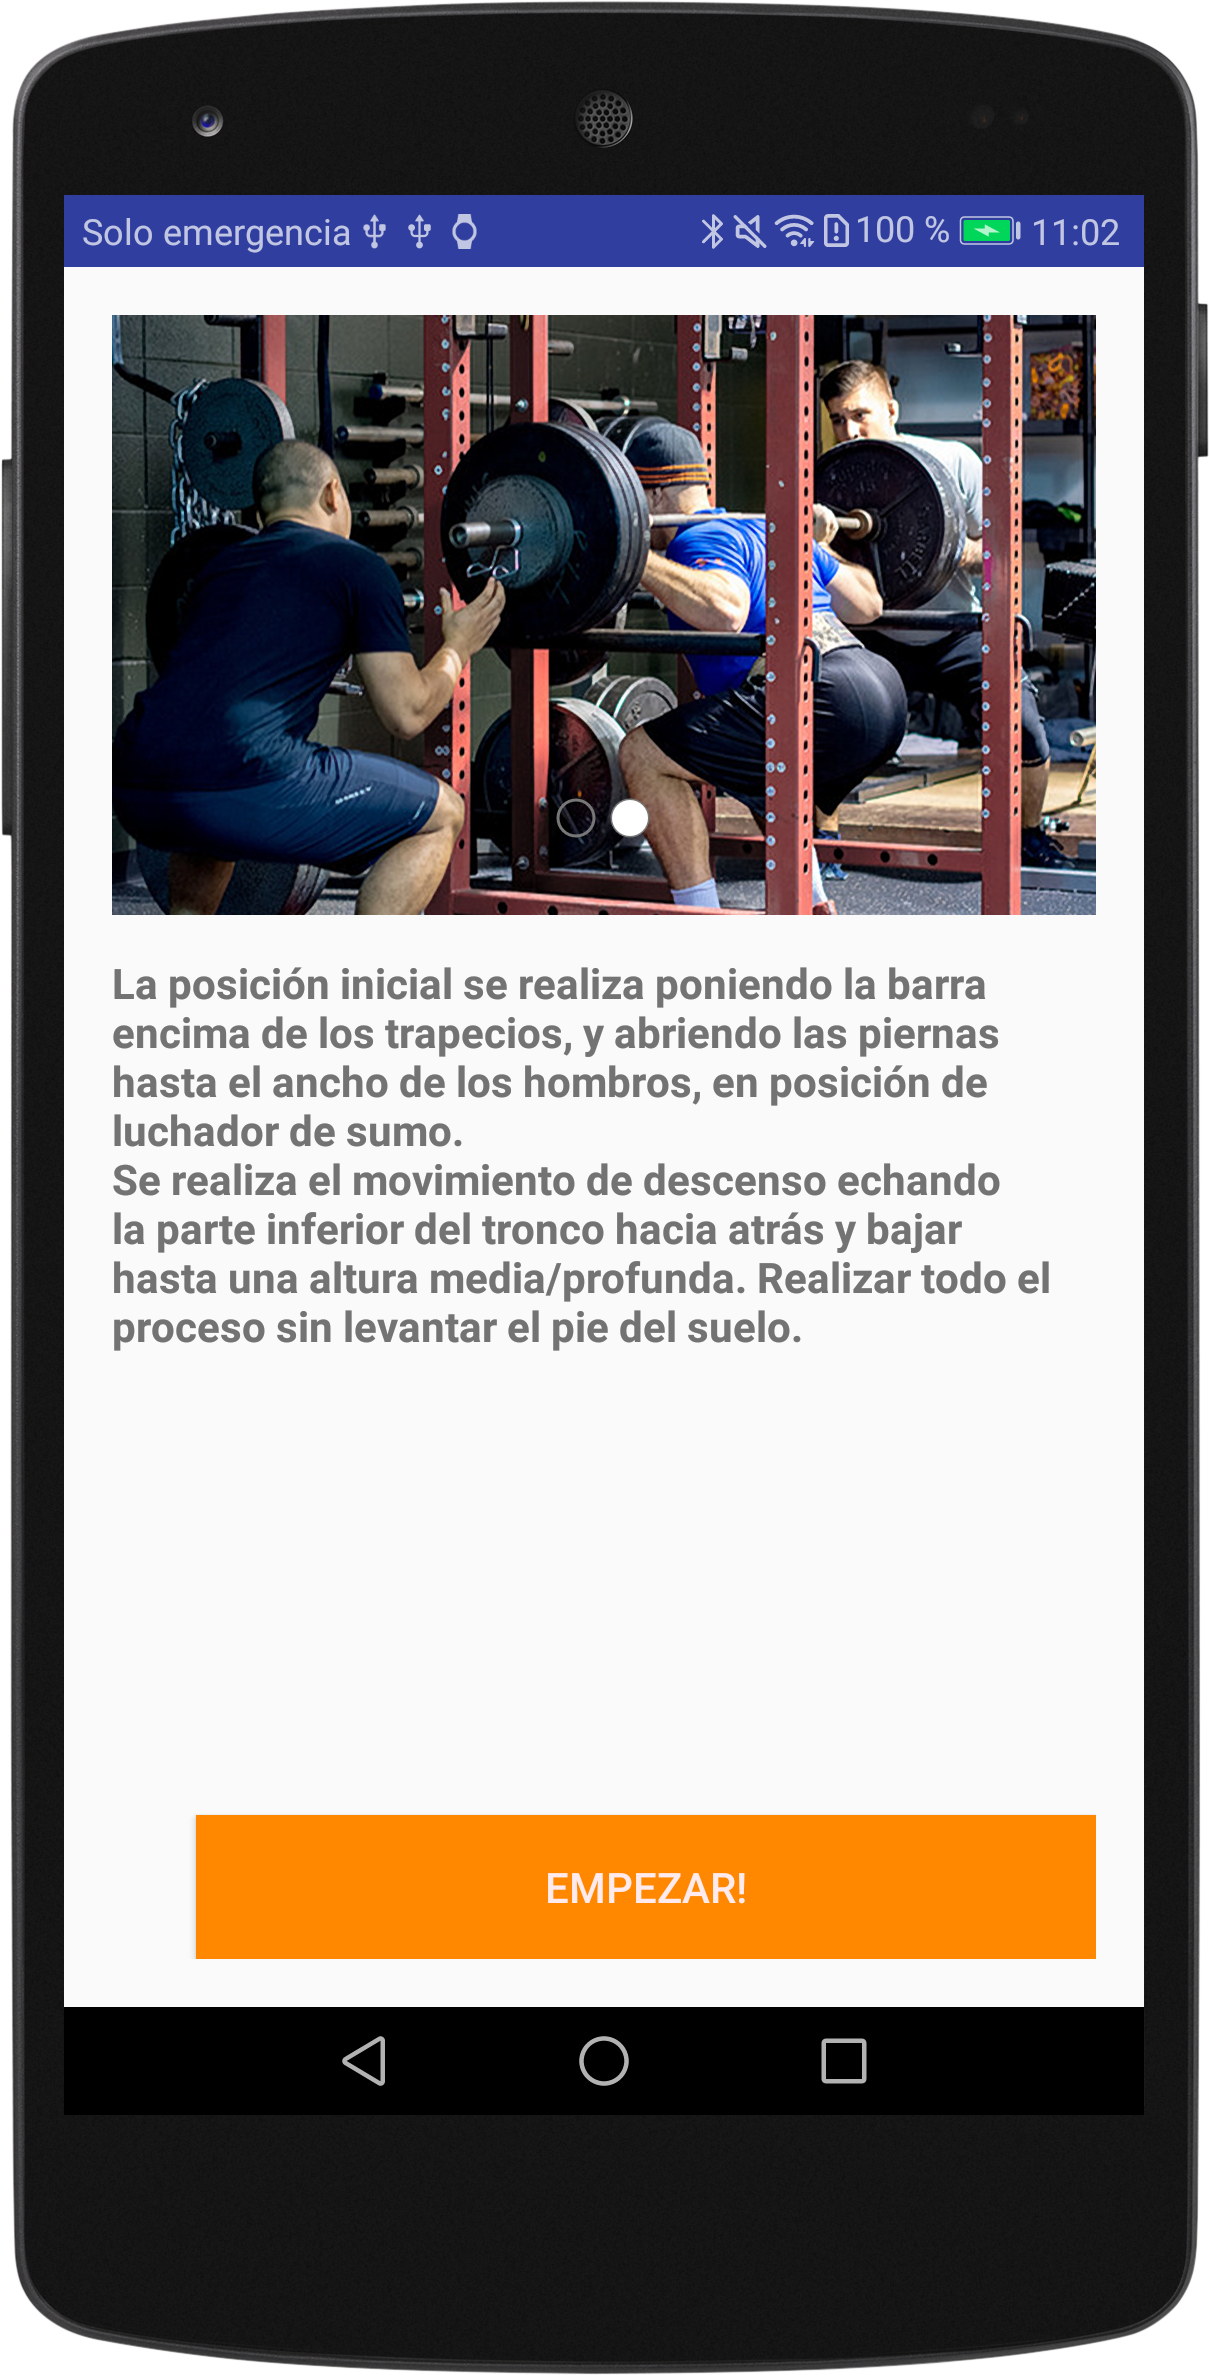
\includegraphics[scale=0.10]{imagenes/m5.png}
	\caption{Vista descripción ejercicio móvil}
	\label{Vista descripción ejercicio movil}
\end{figure}

\begin{figure}[H]
	\centering
	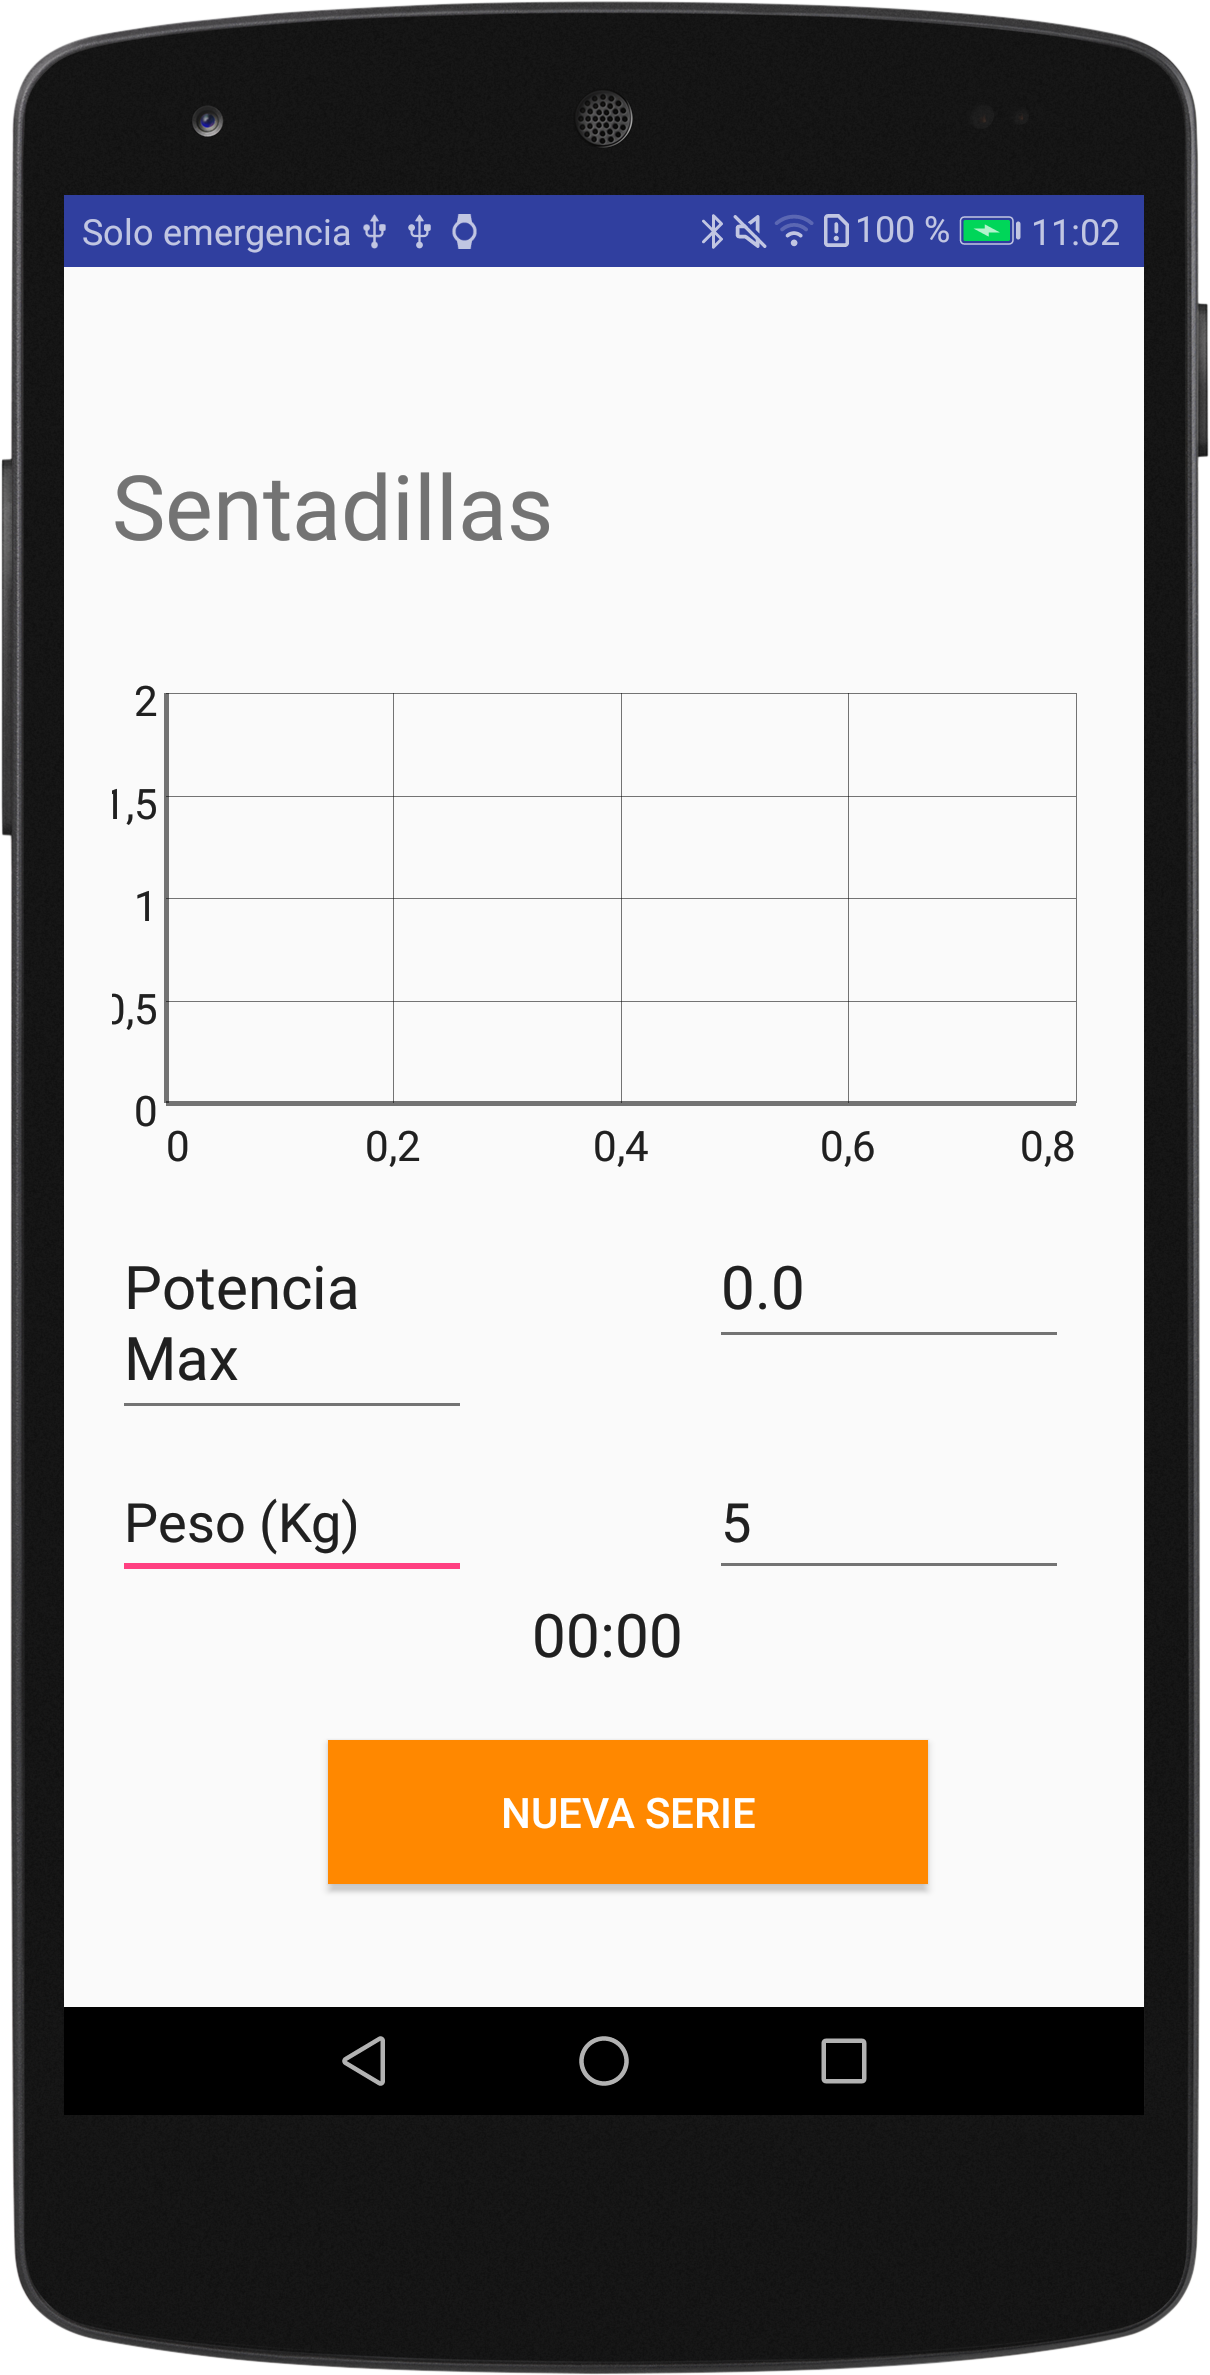
\includegraphics[scale=0.10]{imagenes/m6.png}
	\caption{Vista inicial ejercicio móvil}
	\label{Vista inicial ejercicio movil}
\end{figure}

\begin{figure}[H]
	\centering
	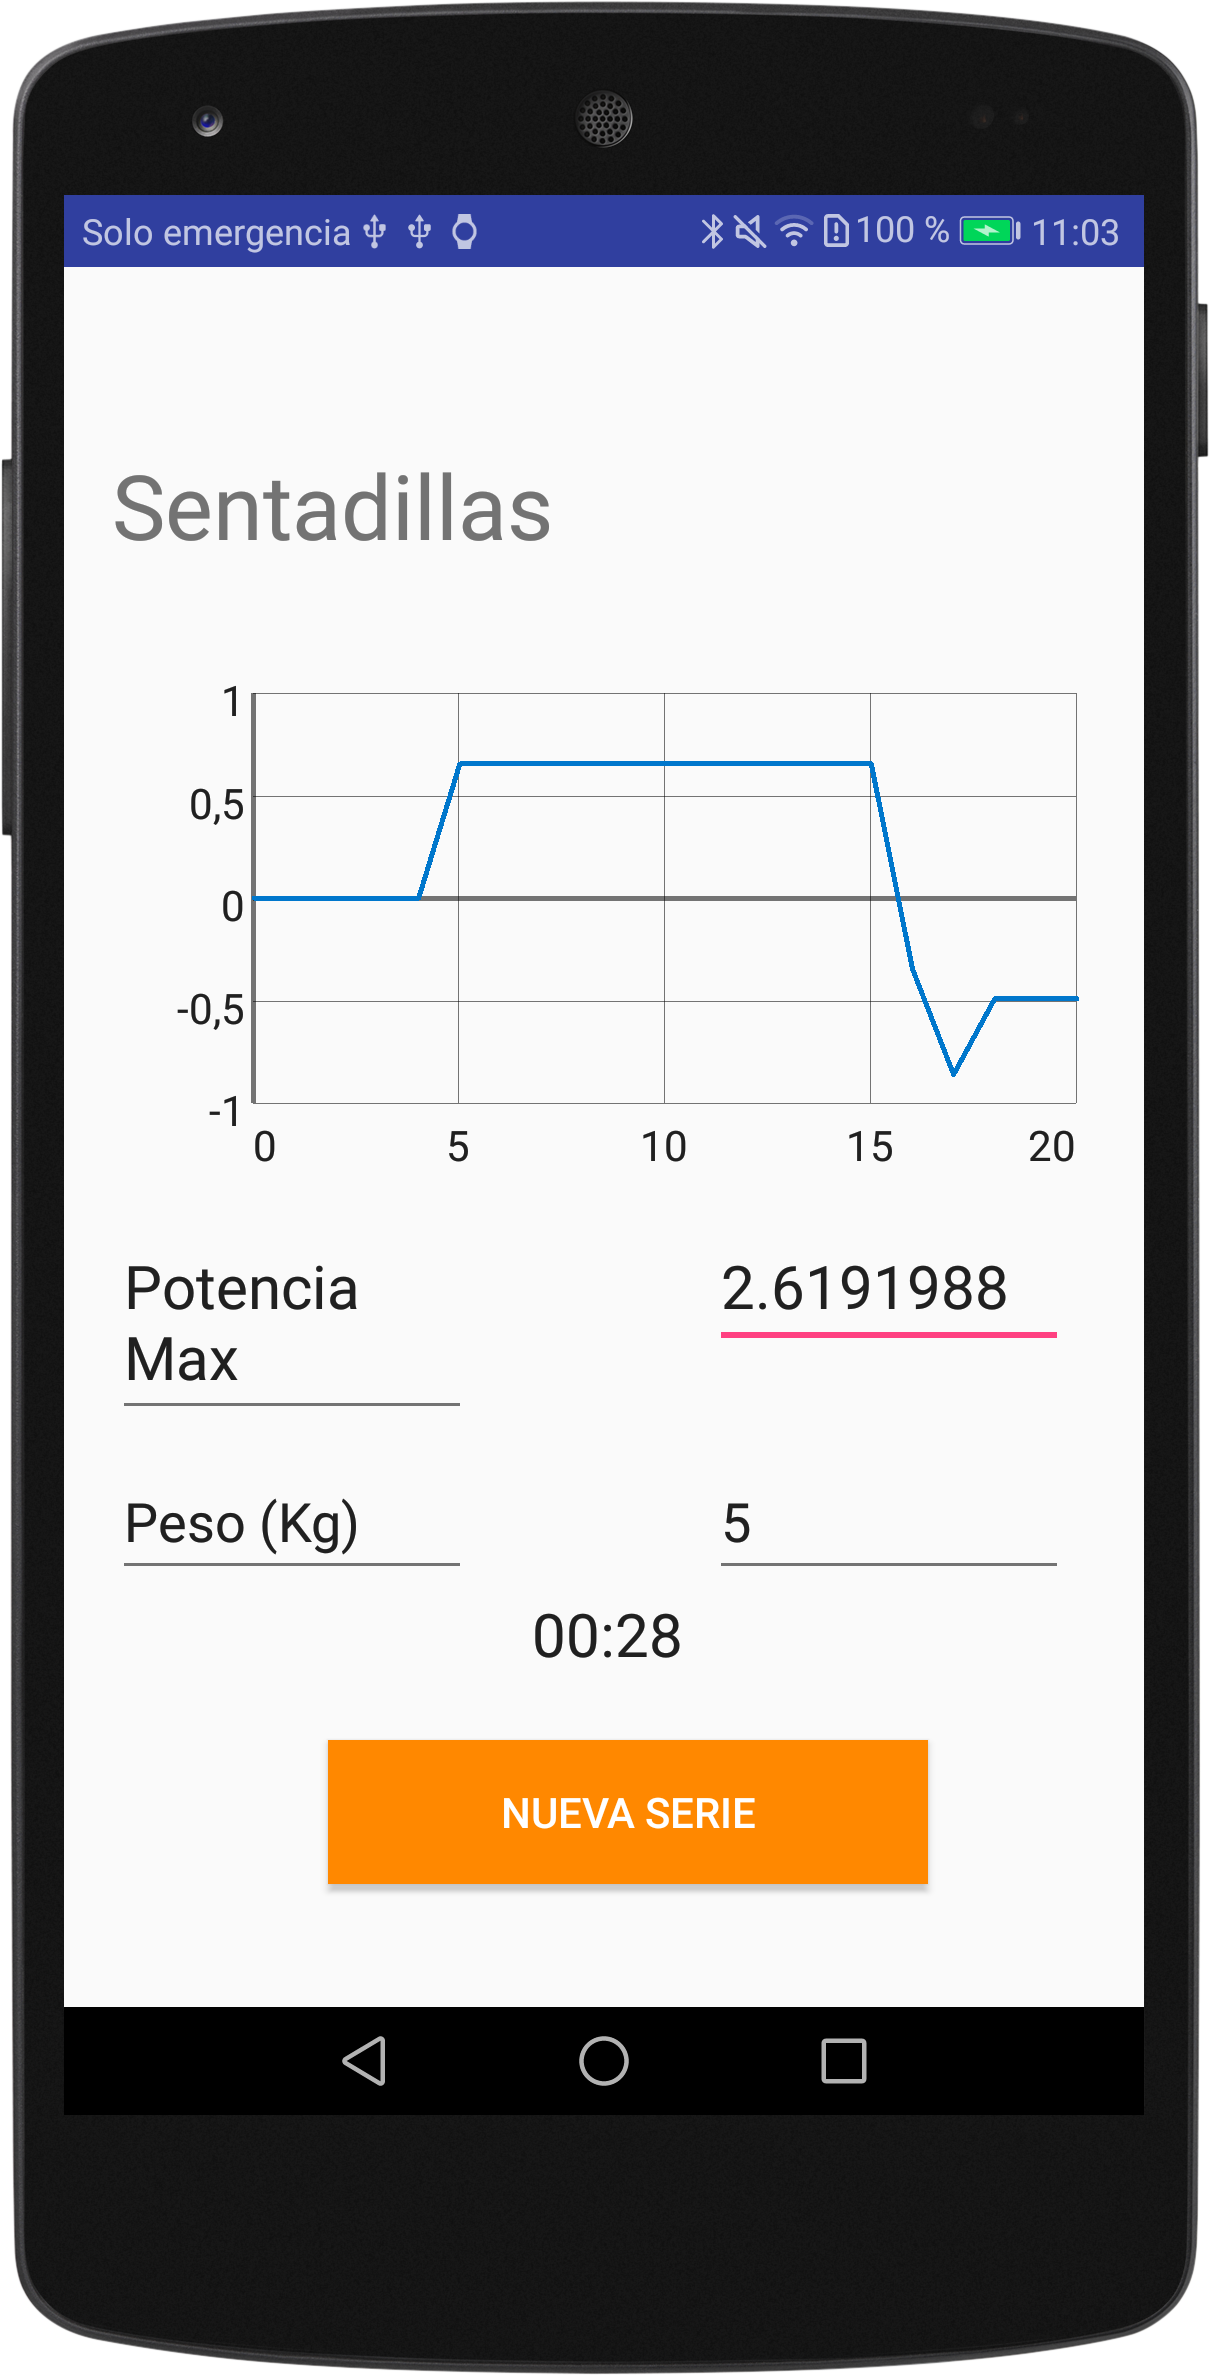
\includegraphics[scale=0.10]{imagenes/m7.png}
	\caption{Vista realización ejercicio móvil}
	\label{Vista realización ejercicio movil}
\end{figure}

%
\chapter{Pruebas}

En este capítulo se va a analizar como se comporta la aplicación frente a un escenario real, con el fin de apreciar la fiabilidad con la que representa la potencia.
\\
\\
Para ello se han realizado unas mediciones con la aplicación en una máquina 'multipower' (smith machine), utilizando una escala para medir la distancia con respecto al tiempo, haciendo uso de una cámara (no de alta velocidad). Se ha a procedido a calcular la velocidad real media y la velocidad calculada, con el fin de ver cual es la diferencia. Puesto que el cálculo de la velocidad es el que más error implica en nuestro sistema.

\begin{figure}[H]
	\centering
	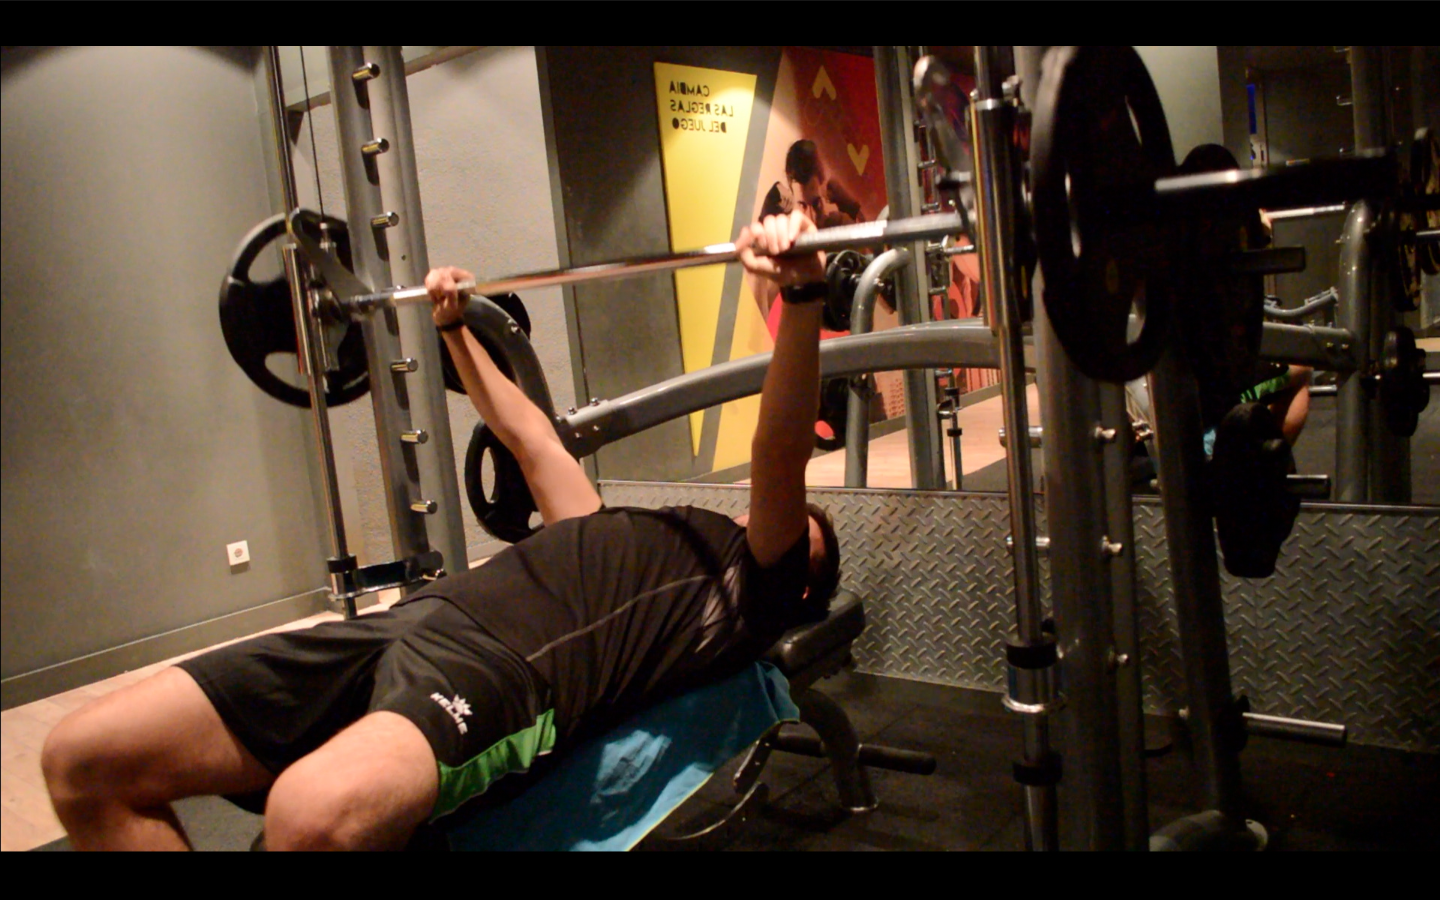
\includegraphics[scale=0.2]{imagenes/prueba1.png}
	\caption{Realización del primer test de la aplicación.}
	\label{Realización test}
\end{figure}

\section*{Test 1}

Se realizó una serie con 3 repeticiones.


\begin{table}[H]
\centering
\caption{Test 1}
\label{Test 1}
\begin{tabular}{|l|l|l|l|}
\hline
Tiempo (s) & Velocidad media real (m/s) & Velocidad media calculada (m/s) & Diferencia \\ \hline
1          & 0,175                      & 0                               & 0,175      \\ \hline
2          & 0,175                      & 0,11                            & 0,065      \\ \hline
3          & 0,175                      & 0,19                            & 0,015      \\ \hline
4          & 0,08                       & 0,21                            & 0,1225     \\ \hline
5          & 0,08                       & 0,35                            & 0,27       \\ \hline
6          & 0,262                      & 0,35                            & 0,08       \\ \hline
7          & 0,087                      & 0,76                            & 0,67       \\ \hline
8          & 0,22                       & 0,28                            & 0,06       \\ \hline
9          & 0,17                       & 0,28                            & 0,11       \\ \hline
10         & 0,25                       & 0,43                            & 0,18       \\ \hline
\end{tabular}
\end{table}

\section*{Test 2}

Esta vez se realizó una sola repetición. Para evaluar el comportamiento de la aplicación a baja velocidad.

\begin{table}[H]
\centering
\caption{Test 2}
\label{Test 2l}
\begin{tabular}{|l|l|l|l|}
\hline
Tiempo (s) & Velocidad media real (m/s) & Velocidad media calculada (m/s) & Diferencia \\ \hline
1          & 0                          & 0                               & 0          \\ \hline
2          & 0                          & 0                               & 0          \\ \hline
3          & 0                          & 0,190                           & 0,190      \\ \hline
4          & 0                          & 0,26                            & 0,26       \\ \hline
5          & 0,05                       & 0,26                            & 0,21       \\ \hline
6          & 0,10                       & 0,26                            & 0,16       \\ \hline
7          & 0,076                      & 0,15                            & 0,12       \\ \hline
8          & 0,05                       & 0,15                            & 0,10       \\ \hline
9          & 0,05                       & 0,15                            & 0,10       \\ \hline
10         & 0,03                       & 0,27                            & 0,24       \\ \hline
\end{tabular}
\end{table}

\section*{Test 3}

Se realizaron 15 repeticiones a lo largo de 40 segundos. Evaluando así el comportamiento de la aplicación en series largas.

\begin{table}[H]
\centering
\caption{Test 3}
\label{Test 3}
\begin{tabular}{|l|l|l|l|}
\hline
Tiempo (s) & Velocidad media real (m/s) & Velocidad media calculada (m/s) & Diferencia \\ \hline
0          & 0                          & 0                         & 0          \\ \hline
5          & 0.66                       & 0.57                      & 0,09       \\ \hline
10         & 0,96                       & 0,61                      & 0,35       \\ \hline
15         & 0,56                       & 1,43                      & 0,87       \\ \hline
20         & 0,54                       & 1,16                      & 0,62       \\ \hline
25         & 0,24                       & 1,94                      & 1,7        \\ \hline
30         & 0,64                       & 2,00                      & 1,36       \\ \hline
35         & 0,76                       & 2,31                      & 1,55       \\ \hline
40         & 0,40                       & 2,04                      & 1,64       \\ \hline
\end{tabular}
\end{table}

\noindent
Se puede ver que la aplicación se comporta de manera correcta en tiempo real, sin retardo apreciable por el usuario. Sin embargo la aplicación parece ser poco precisa cuando la velocidad del ejercicio es muy baja y cuando se produce desaceleración. Además la diferencia entre los valores calculados y reales aumenta con el tiempo, produciendo así un error bastante elevado. Esto es debido a que la estimación de la velocidad actual por medio de la integración diverge alejandose de la realidad rápidamente debido al ruido.
\\
\\
A falta de más pruebas, la aplicación es funcional, aunque su cálculo de la potencia es aproximado y contiene un gran margen de error. Por lo que no podemos garantizar que la aplicación realice la monitorización de manera correcta, especialmente cuando el tiempo de la serie es elevado.

%
\chapter{Conclusiones y trabajo futuro}

\section*{Conclusiones}

A la hora de realizar el proyecto, se partía con una serie de objetivos en mente, los cuales se debían conseguir para el correcto funcionamiento de la aplicación. Una vez finalizado el proyecto, no se puede afirmar que los objetivos se hayan conseguido. Pues aún habiendo obtenido una aplicación totalmente operativa y completa, no podemos garantizar que la monitorización del ejercicio sea correcta.
\\
Esto es debido a que la desviación producida al calcular la velocidad diverge rápidamente, a causa del ruido en función del tiempo. Por lo que el error de offset entre la potencia real y potencia monitorizada, aumentará rápidamente conforme el tiempo de realización del ejercicio aumenta. Además, la frecuencia de muestreo en Android puede cambiar a lo largo del tiempo (recibiendo los datos antes o después de la tasa especificada) y no puede ser controlada \cite{SensorGoogle}, produciendo así incoherencia en el cálculo de la velocidad. Lo cual produce que la aplicación solo pueda ser usada en series de 1 a 3 repeticiones y, consecuentemente, inviable en la mayoría de entrenamientos.
\\
Dicha desviación podría ser corregida realizando la asunción de patrones conocidos, como que el usuario realice una parada entre repeticiones. Pero en dicho caso la rutina del usuario estaría condicionada, por lo que no es viable.
\\
\\
Se debe destacar que para la realización de este trabajo fue necesario realizar un estudio sobre la monitorización del movimiento utilizando sensores en un escenario 3D, sus limitaciones y métodos de calibración. Implementando los métodos más prometedores y comparandolos. Sorprendentemente, el algoritmo de orientación de Madgwick, siendo el más prometedor de todos, fue el que peores resultados obtuvo. Aparentemente, sobre el sistema operativo Android parece no funcionar tan bien, debido principalmente a que la frecuencia de muestreo en Android es orientativa, el desarrollador no tiene control absoluto sobre la frecuencia de muestreo y además, varía con el tiempo. Lo cual afecta mucho a la precisión de algunos algoritmos de calibración y posicionamiento.

\section*{Trabajo futuro}

La aplicación aún siendo funcional presenta una serie de limitaciones. Las cuales se podrán intentar resolver con las siguientes propuestas (ordenadas por prioridad):

\begin{itemize}
  \item Mejora de la calibración de los sensores. Utilizando otras técnicas con el fin de obtener mayor precisión.
  \item Empleo de sensores de mayor calidad.
  \item Creación de un backend propio con una API Rest. Si bien es cierto que Firebase nos proporciona muchas funcionalidades y servicios. El plan gratuito del servicio habilita hasta 100 conexiones simultáneas. Lo cual se traduce en un cuello de botella.
  \item Mejora de las interfaces de usuario. Tanto de la aplicación móvil como wear, con el fin de mejorar la experiencia de usuario.
\end{itemize}

%
%%\chapter{Conclusiones y Trabajos Futuros}
%
%
%%\nocite{*}
\bibliography{bibliografia}\addcontentsline{toc}{chapter}{Bibliografía}
\bibliographystyle{unsrt}
%\bibliographystyle{miunsrturl}
%
\appendix
\chapter{Manual de usuario}

\section{Instalación}

Para poder instalar la aplicación será necesario disponer de una versión de Android igual o superior a la versión 4.4 de Android, puesto que necesitamos compatibilidad con Android Wear. Se debe además disponer de un dispositivo que utilice Android Wear 1.0 o superior.\\
\\
\subsection*{Móvil}
Para instalar la aplicación en un terminal se debe transferir a dicho terminal el archivo apk. Una vez se encuentra en el dispositivo, se debe habilitar la instalación desde origenes desconocidos. Para ello se deberá acceder a la opción de ajustes/seguridad y activar la opción de aplicaciones de origen desconocido.

\begin{figure}[H]
	\centering
	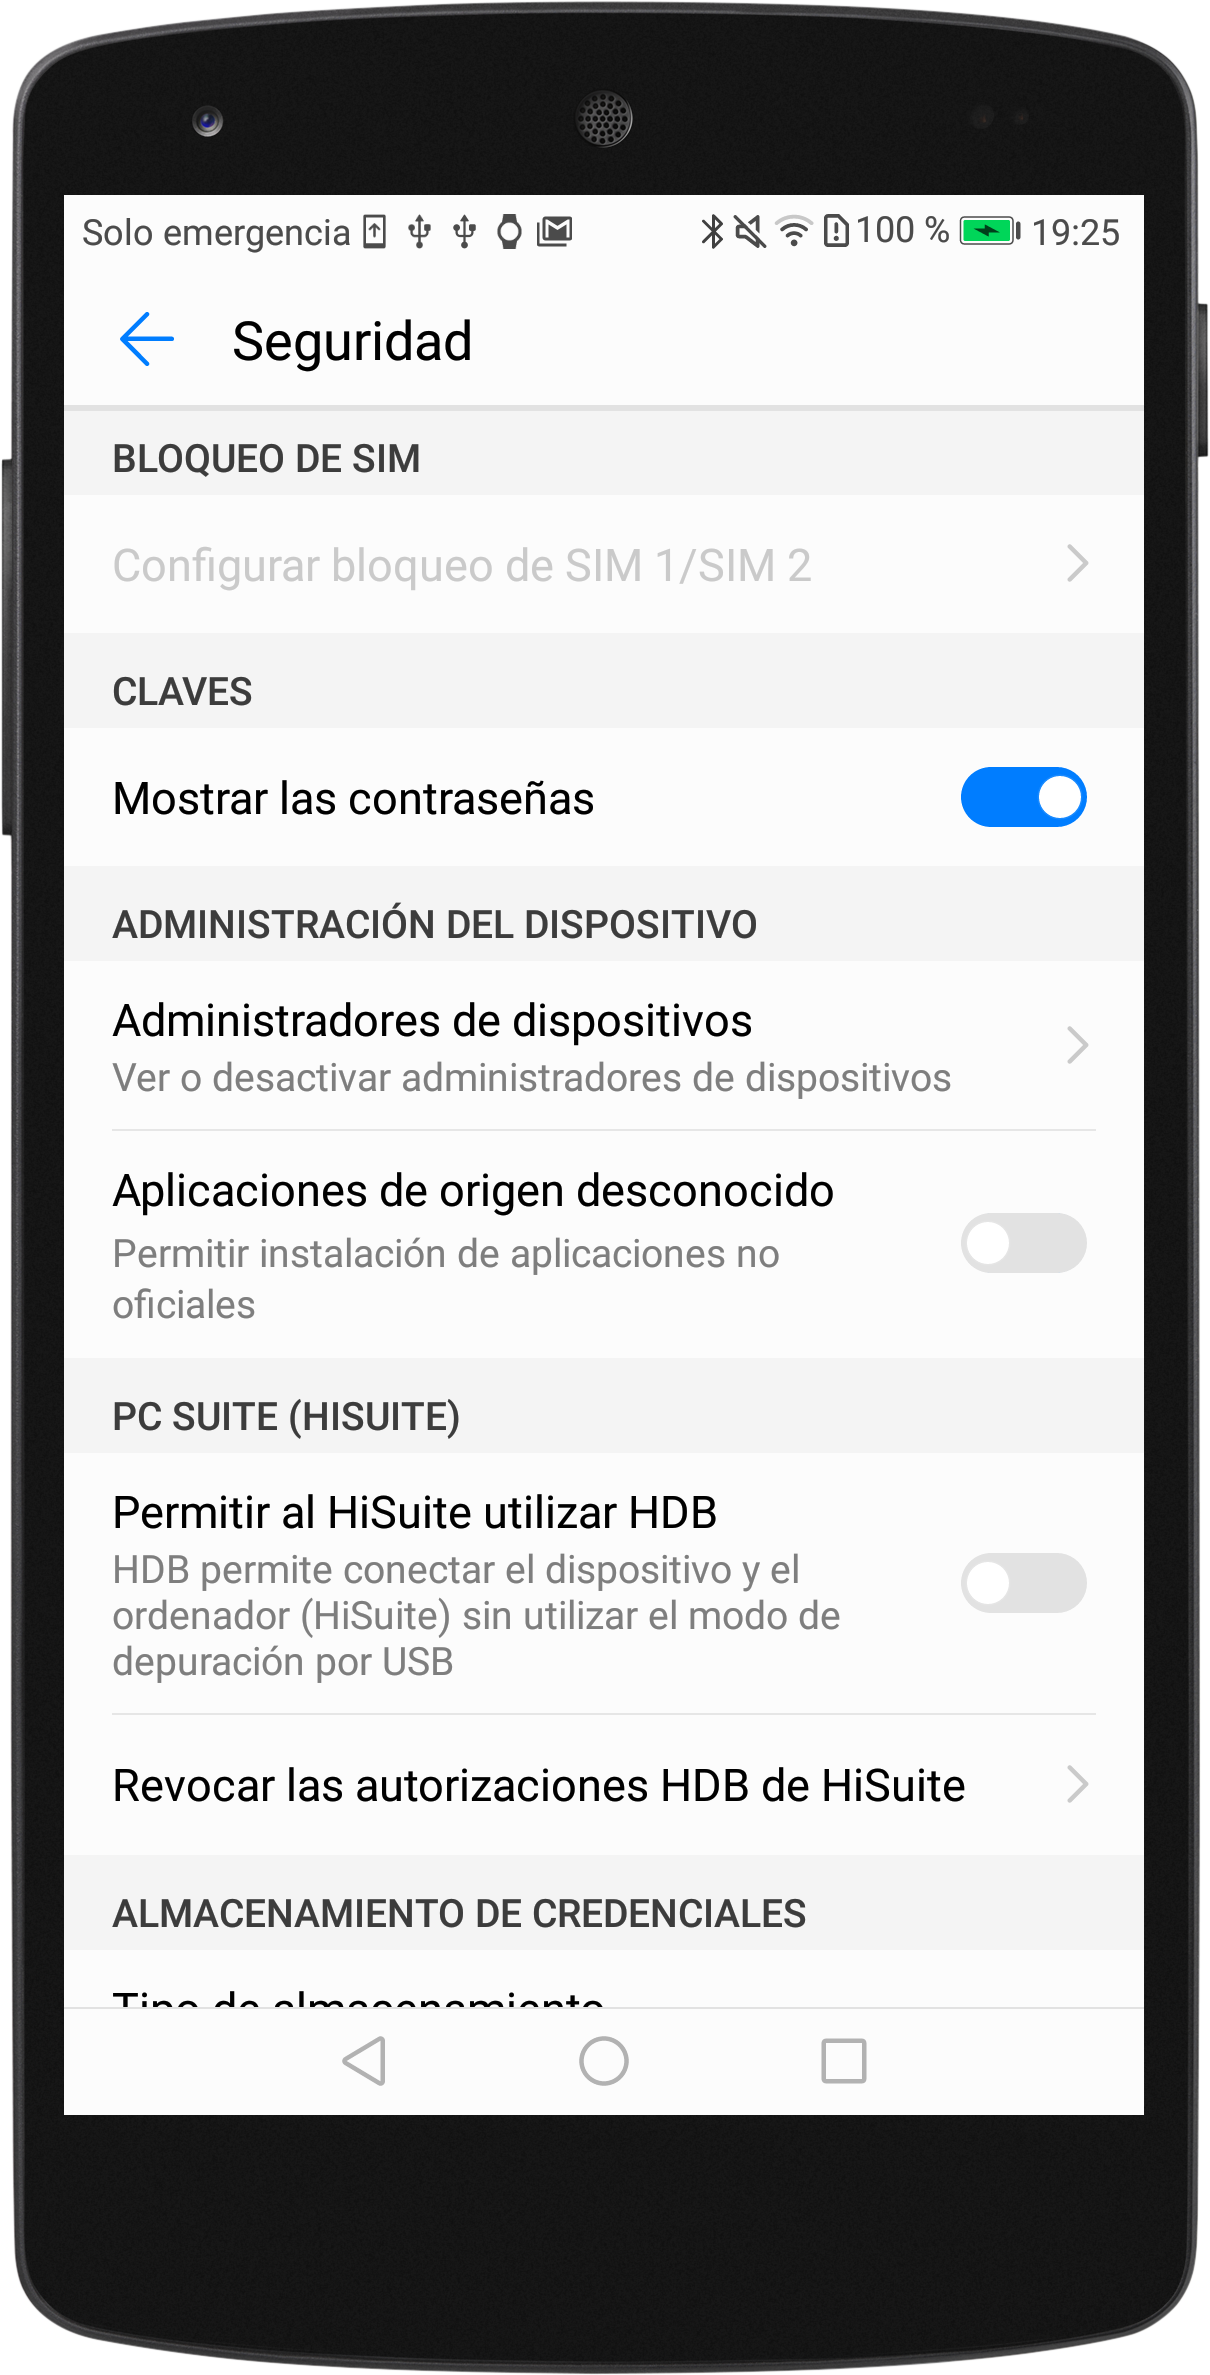
\includegraphics[scale=0.17]{imagenes/seguridad.png}
	\caption{Instalación desde origen desconocido.}
	\label{Instalación desde origen desconocido}
\end{figure}

Una vez esta la opción habilitada, simplemente se tendrá que seleccionar el apk desde el explorador de archivos por defecto y se procederá a su instalación.

\subsection*{Wear}

Para instalar la aplicación en el dispositivo wearable, se deberá activar las opciones de desarrollador del dispositivo, para ello se debe acceder a la opcion de información y seleccionando repetidas veces sobre el número de compilación se podrá acceder a las opciones de desarrollador. Una vez activadas las opciones de desarrollador se deberá permitir la depuración en el dispositivo.


\begin{figure}[H]
	\centering
	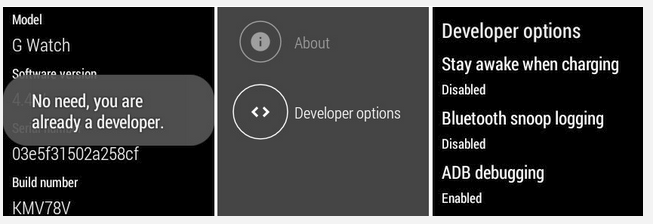
\includegraphics[scale=0.5]{imagenes/dev.png}
	\caption{Modo depuración Android Wear \cite{depur}.}
	\label{Modo depuración Android Wear}
\end{figure}

Con el archivo apk en el ordenador y en el directorio actual, solo quedará ejecutar en un terminal:
\\
\\
\$adb forward tcp:4444 localabstract:/adb–hub \\
\$adb connect localhost:4444 \\
\$adb -e install app.apk \\

\section{Creación de usuario}

Para crear un usuario simplemente se debe abrir la aplicación, hacer click en Registro y rellenar los credenciales necesarios.


\begin{figure}[H]
	\centering
	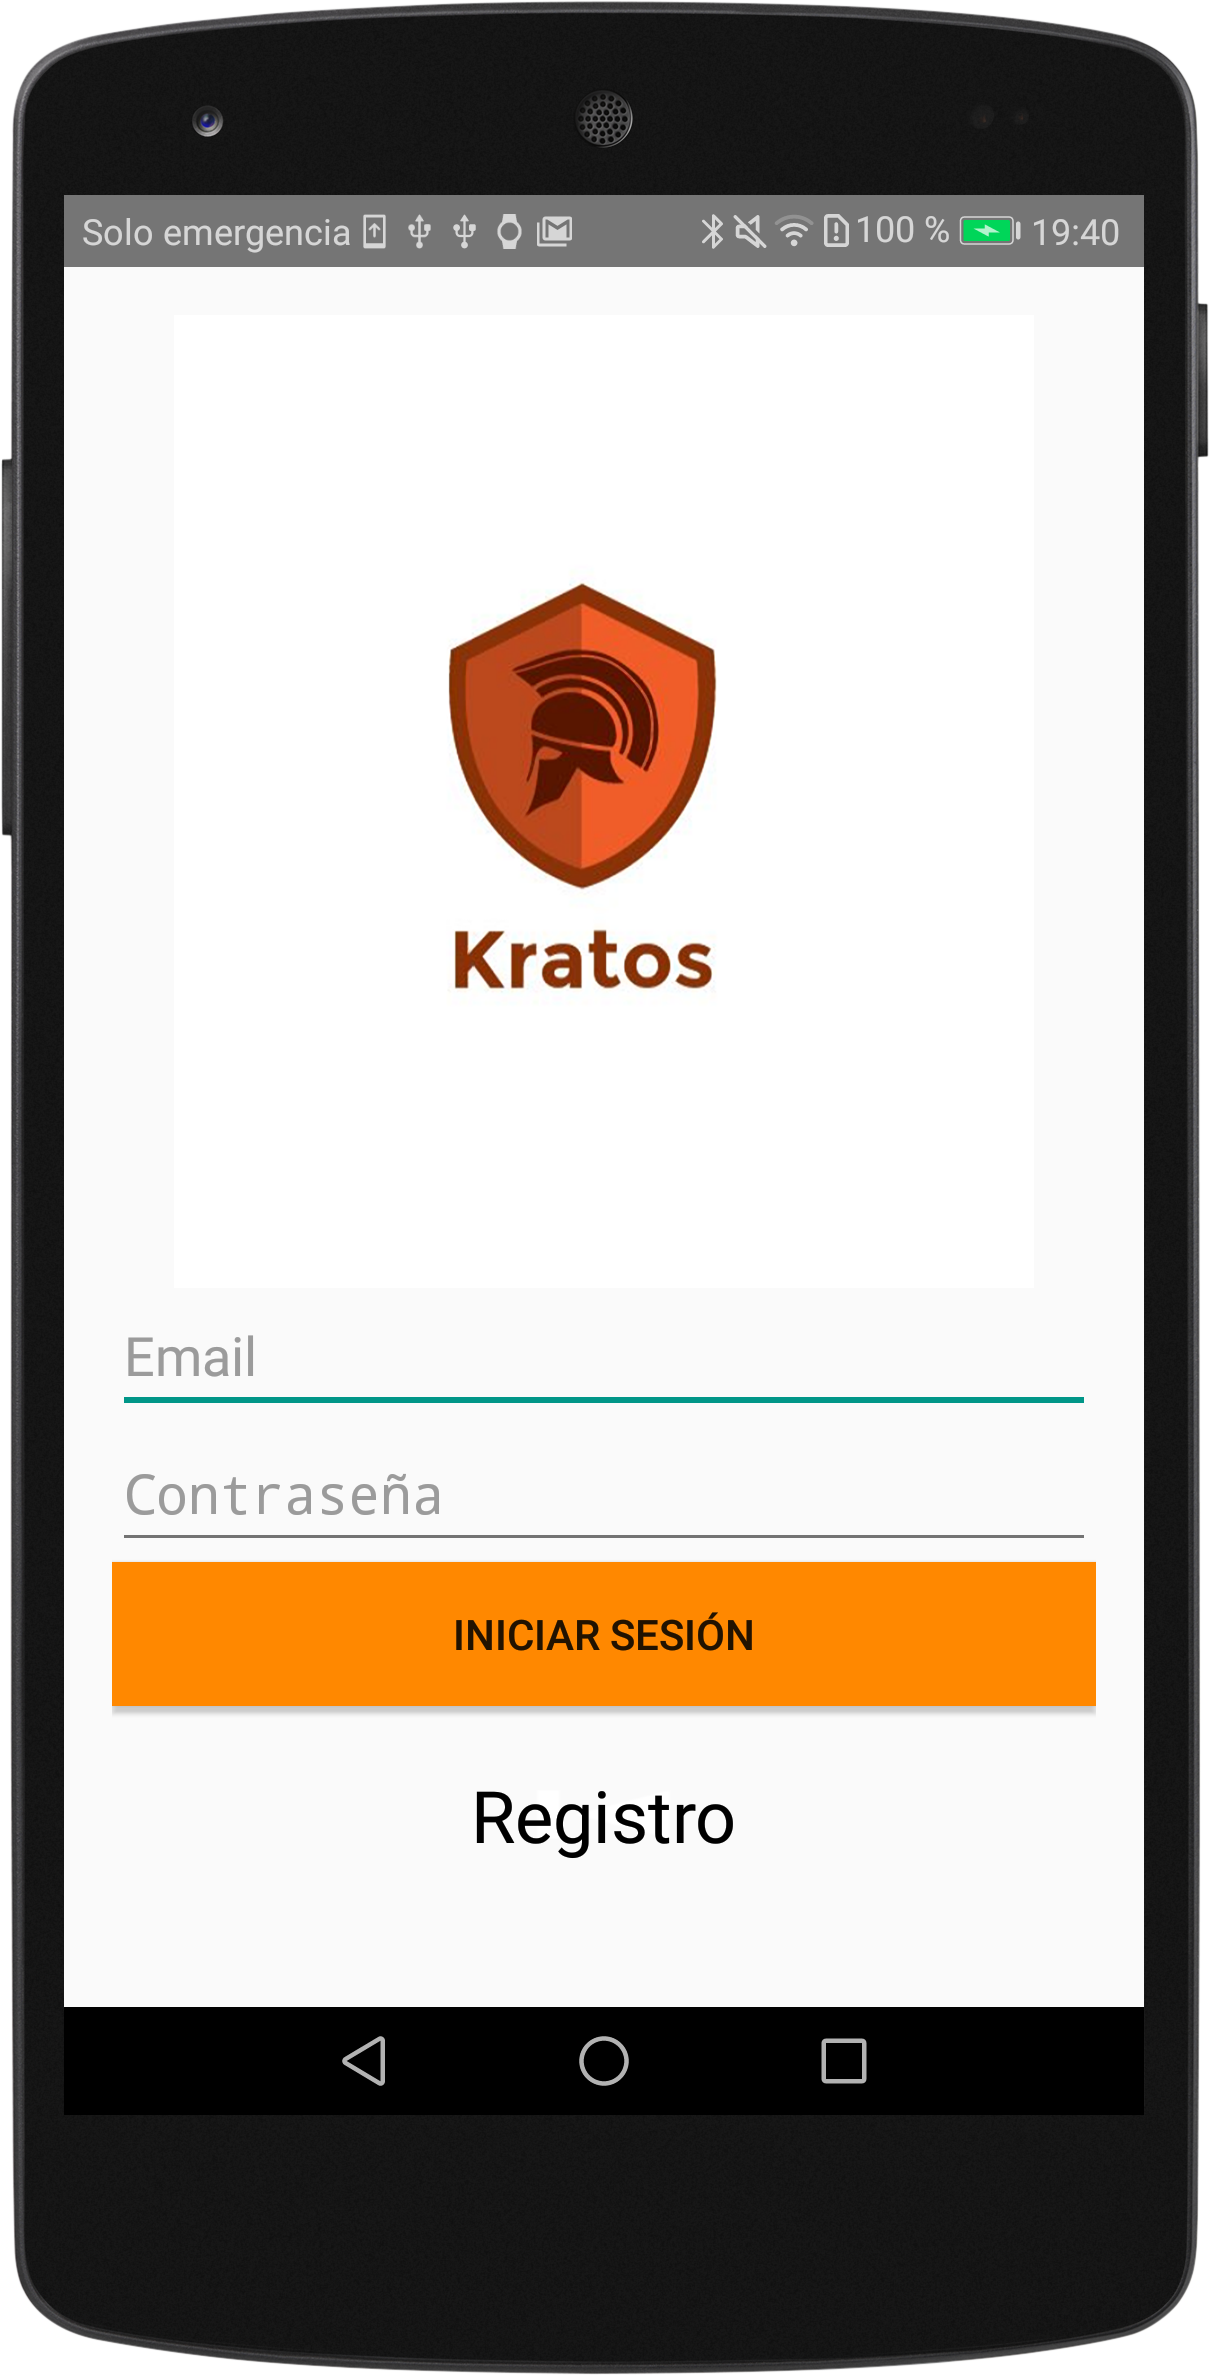
\includegraphics[scale=0.10]{imagenes/m1.png}
	\caption{Regristro 1.}
	\label{Regristro 1}
\end{figure}

\begin{figure}[H]
	\centering
	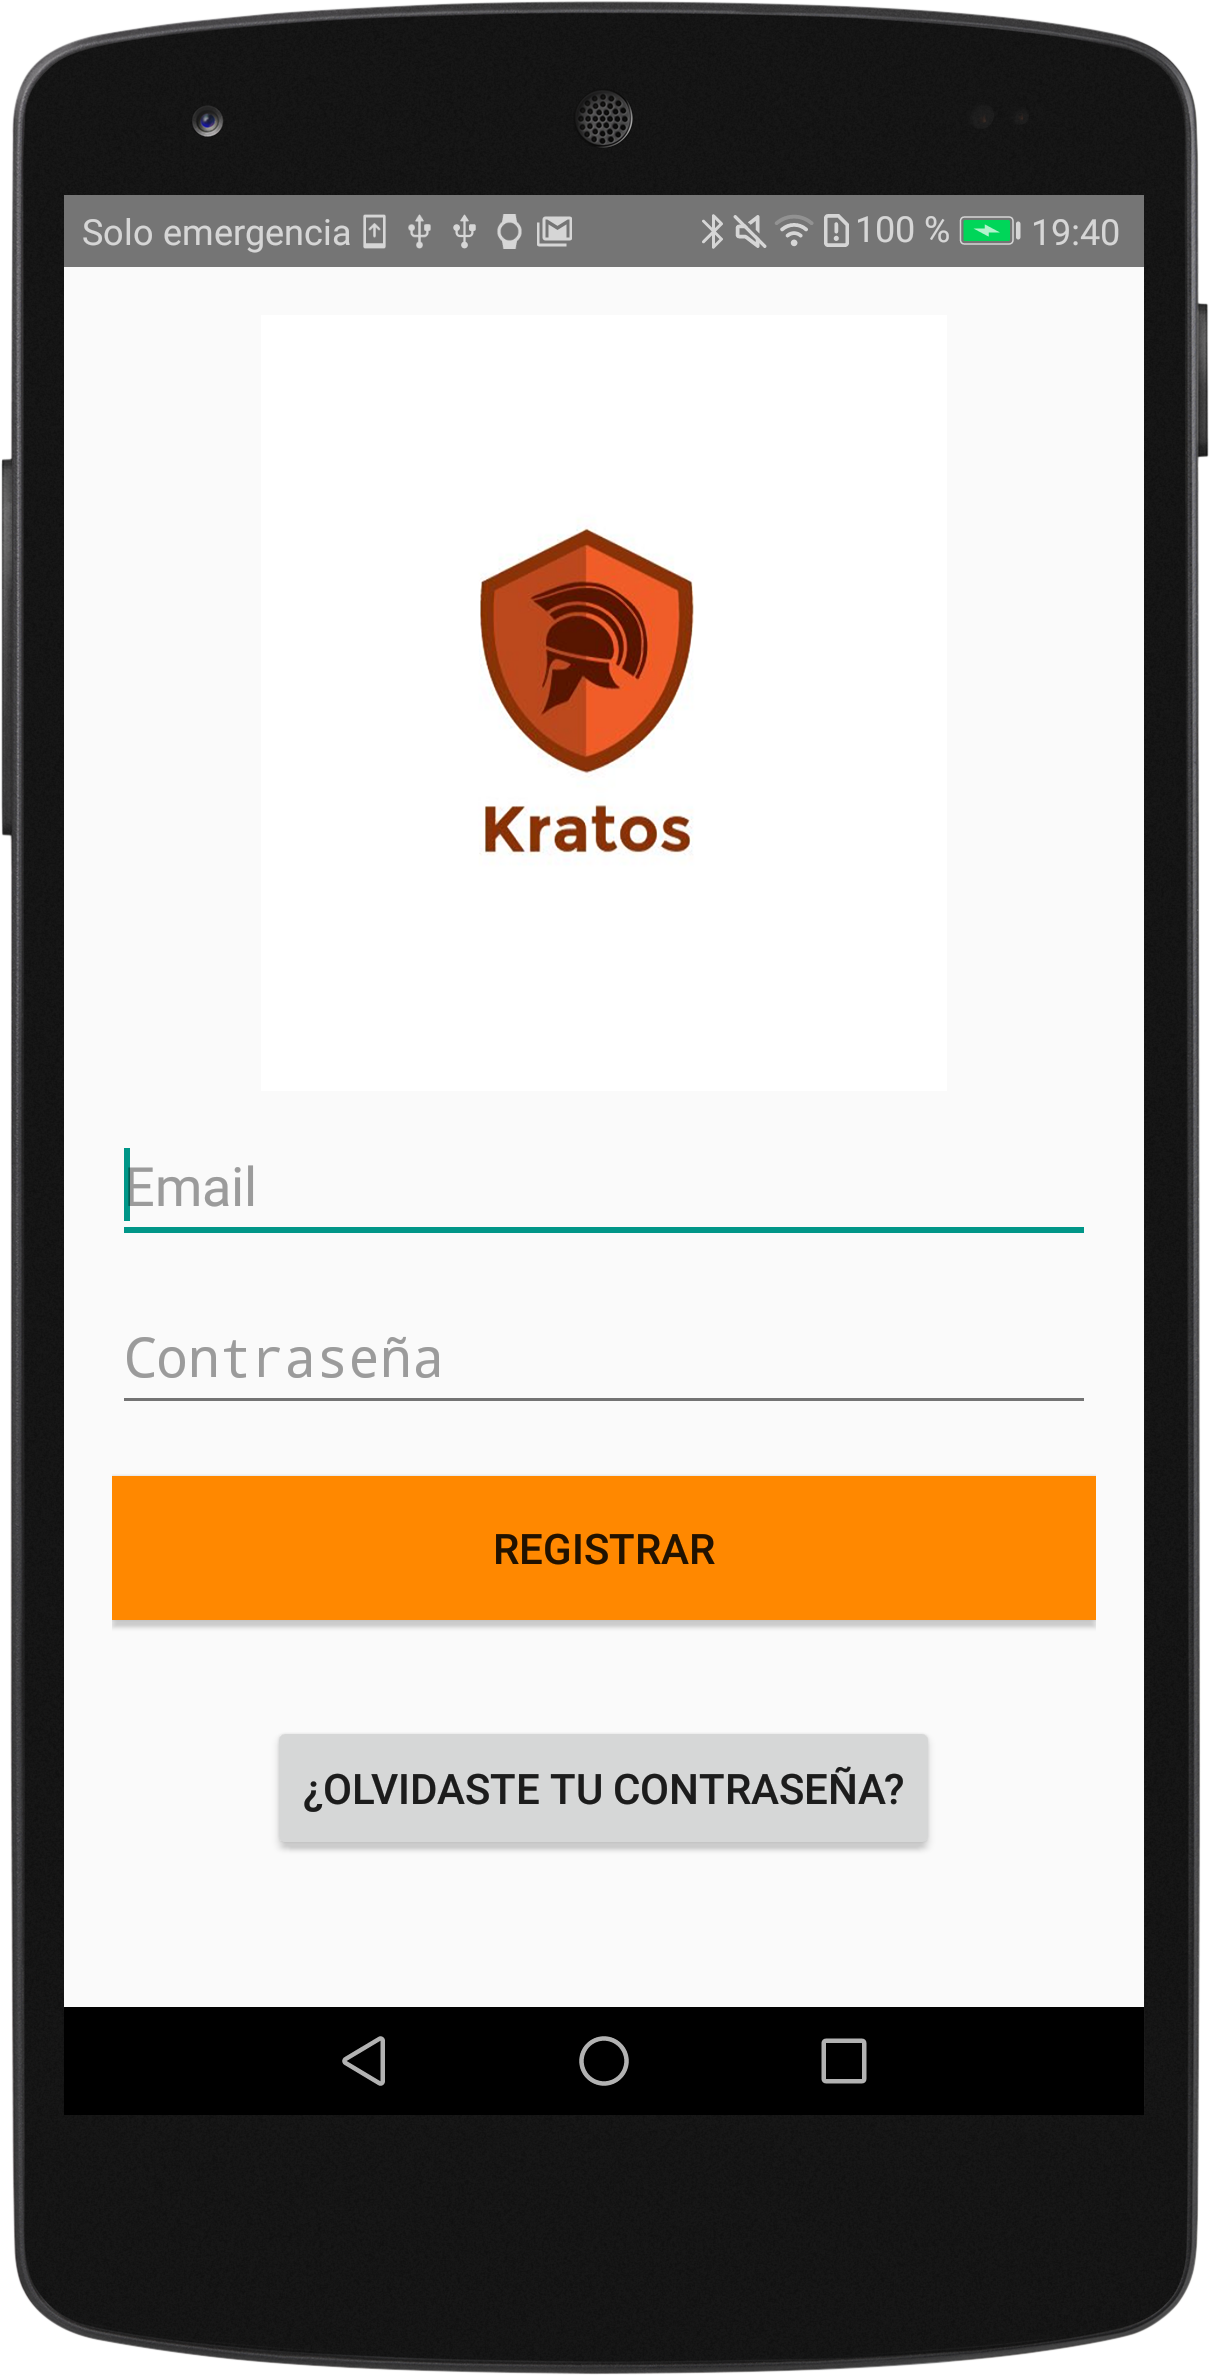
\includegraphics[scale=0.11]{imagenes/registro.png}
	\caption{Regristro 2.}
	\label{Regristro 2}
\end{figure}

\section{Realización ejercicio}

Para realizar la monitorización del ejercicio se debe seleccionar la pestaña ejercicio, seleccionar el ejercicio deseado y empezar el ejercicio. De manera paralela una vez hayamos llegado a la Ejemplo de monitorización, activaremos la aplicación wear y se procederá a realizar el ejercicio.

\begin{figure}[H]
	\centering
	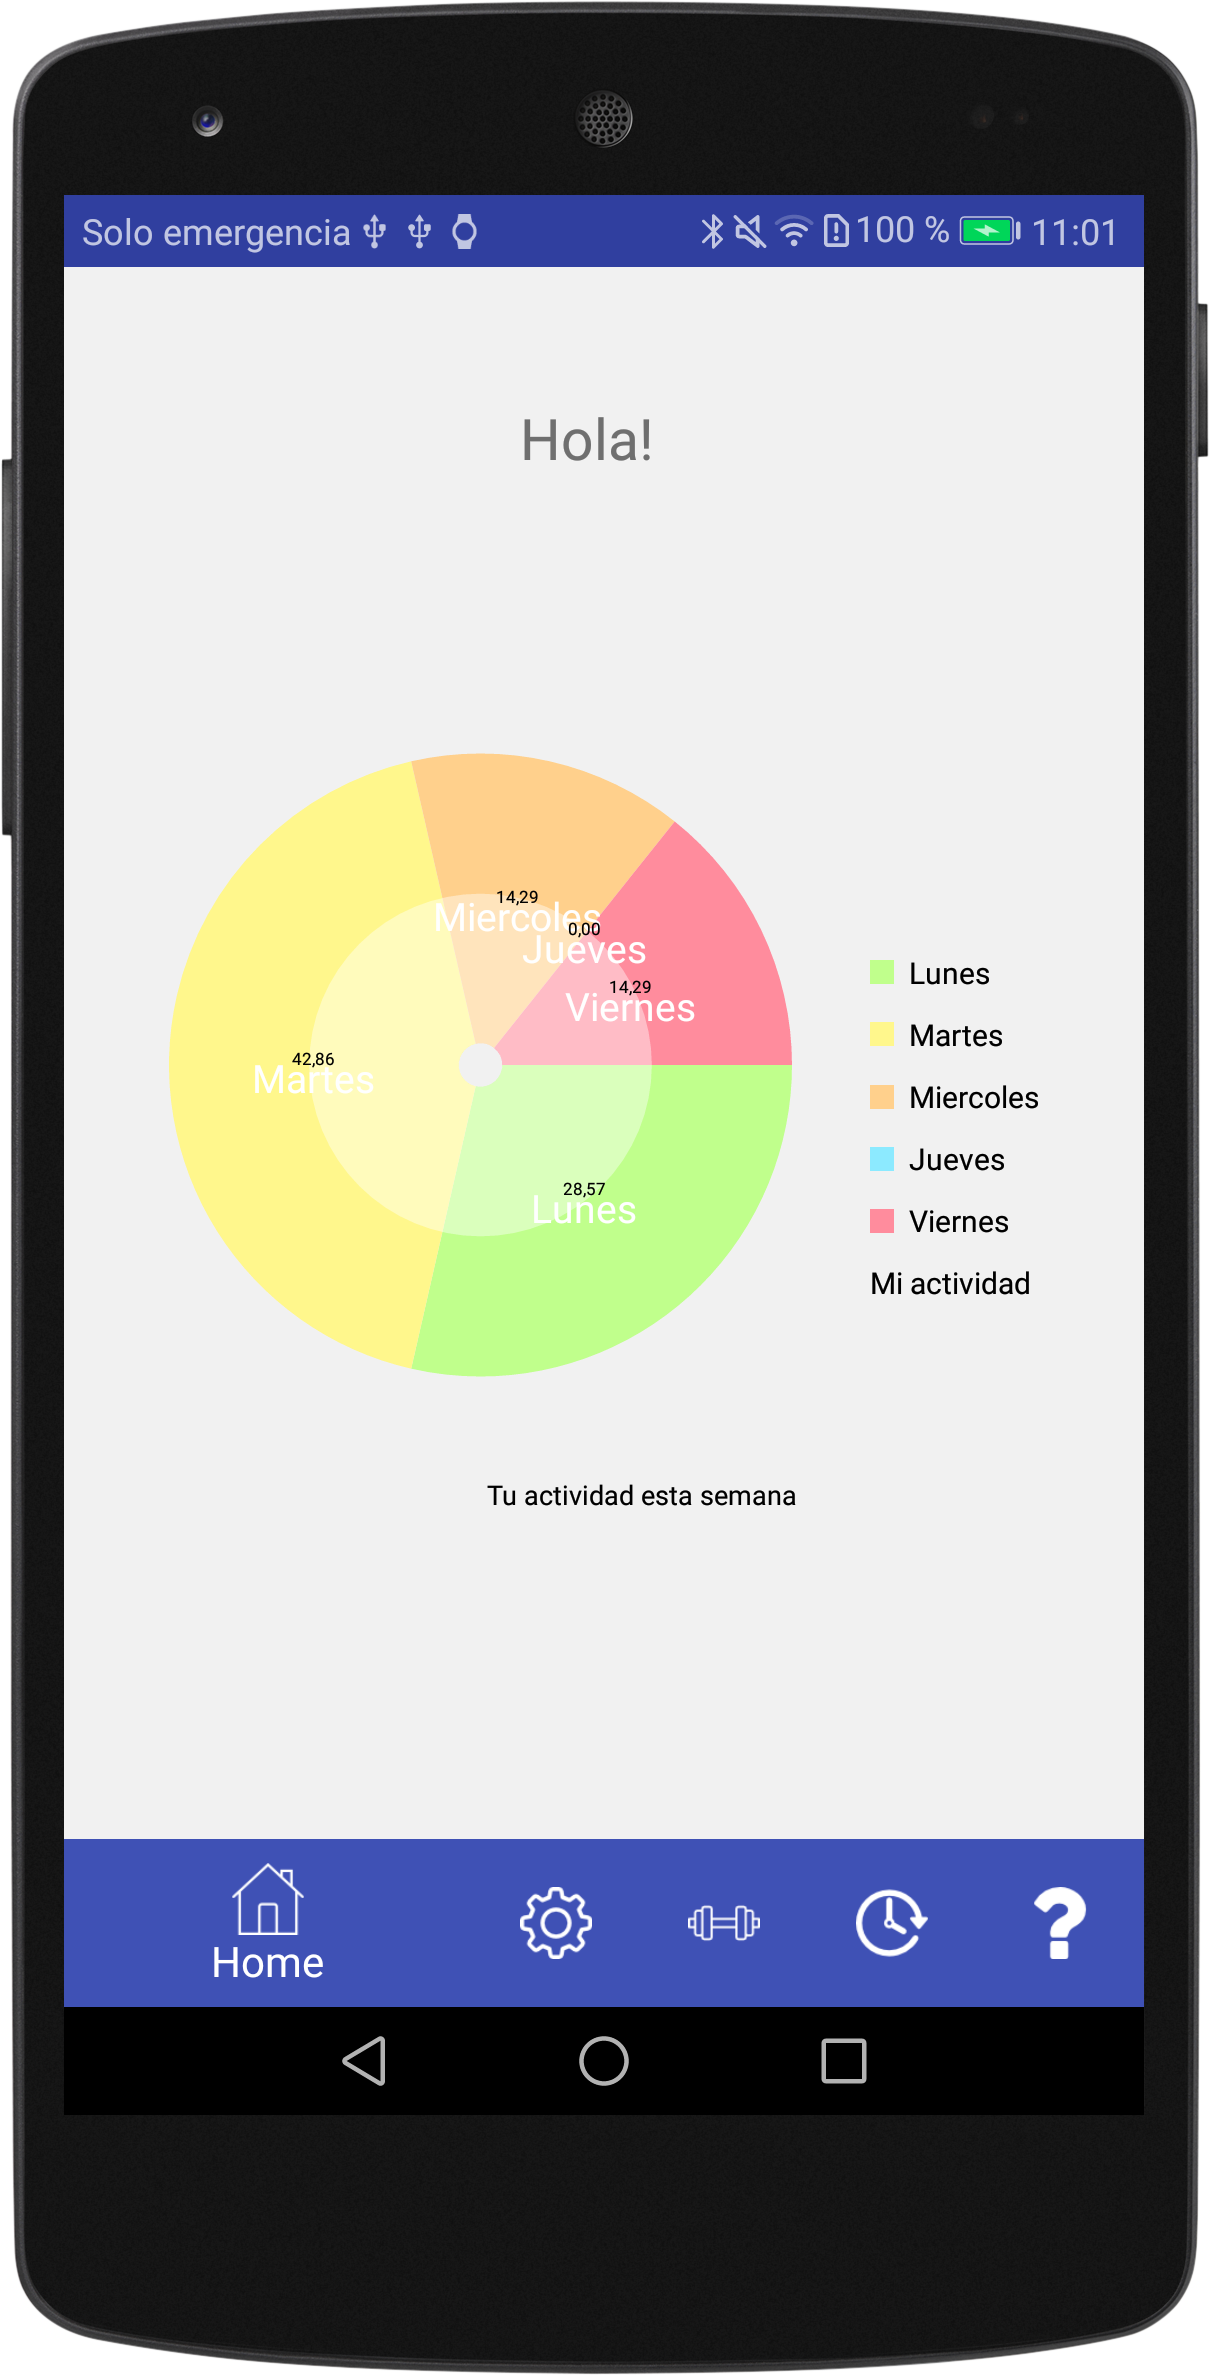
\includegraphics[scale=0.10]{imagenes/m2.png}
	\caption{Pantalla principal móvil}
	\label{Realización ejercicio 1}
\end{figure}


\begin{figure}[H]
	\centering
	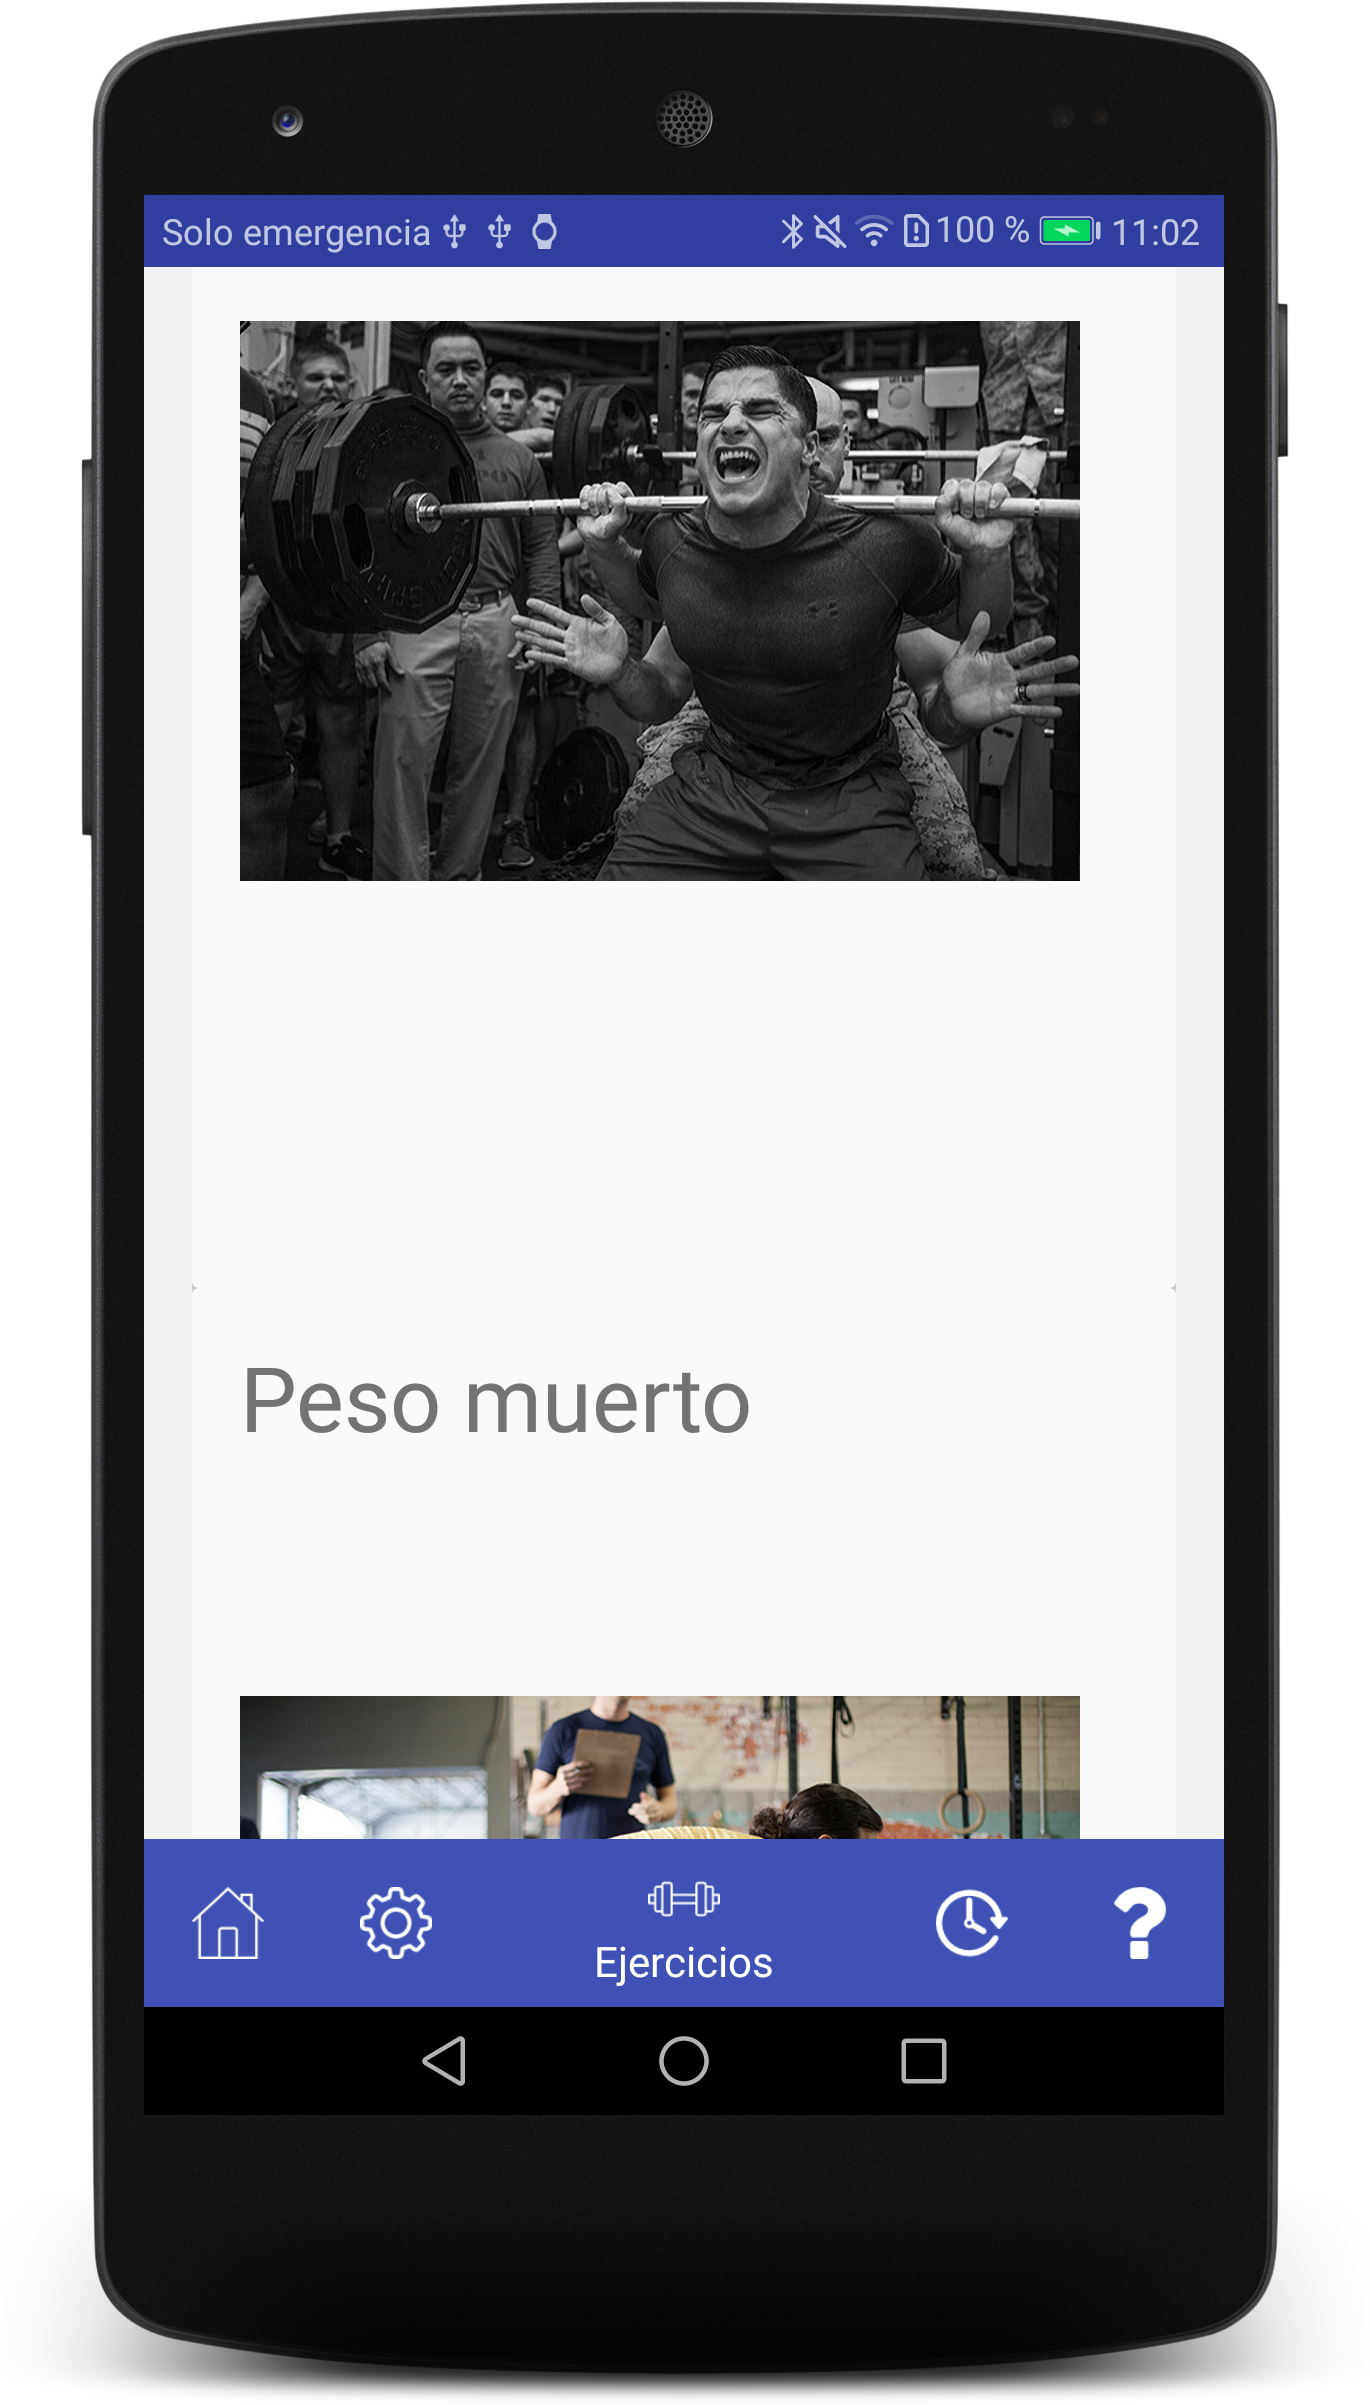
\includegraphics[scale=0.10]{imagenes/m4.png}
	\caption{Ejemplo selección ejercicio móvil}
	\label{Realización ejercicio 2}
\end{figure}

\begin{figure}[H]
	\centering
	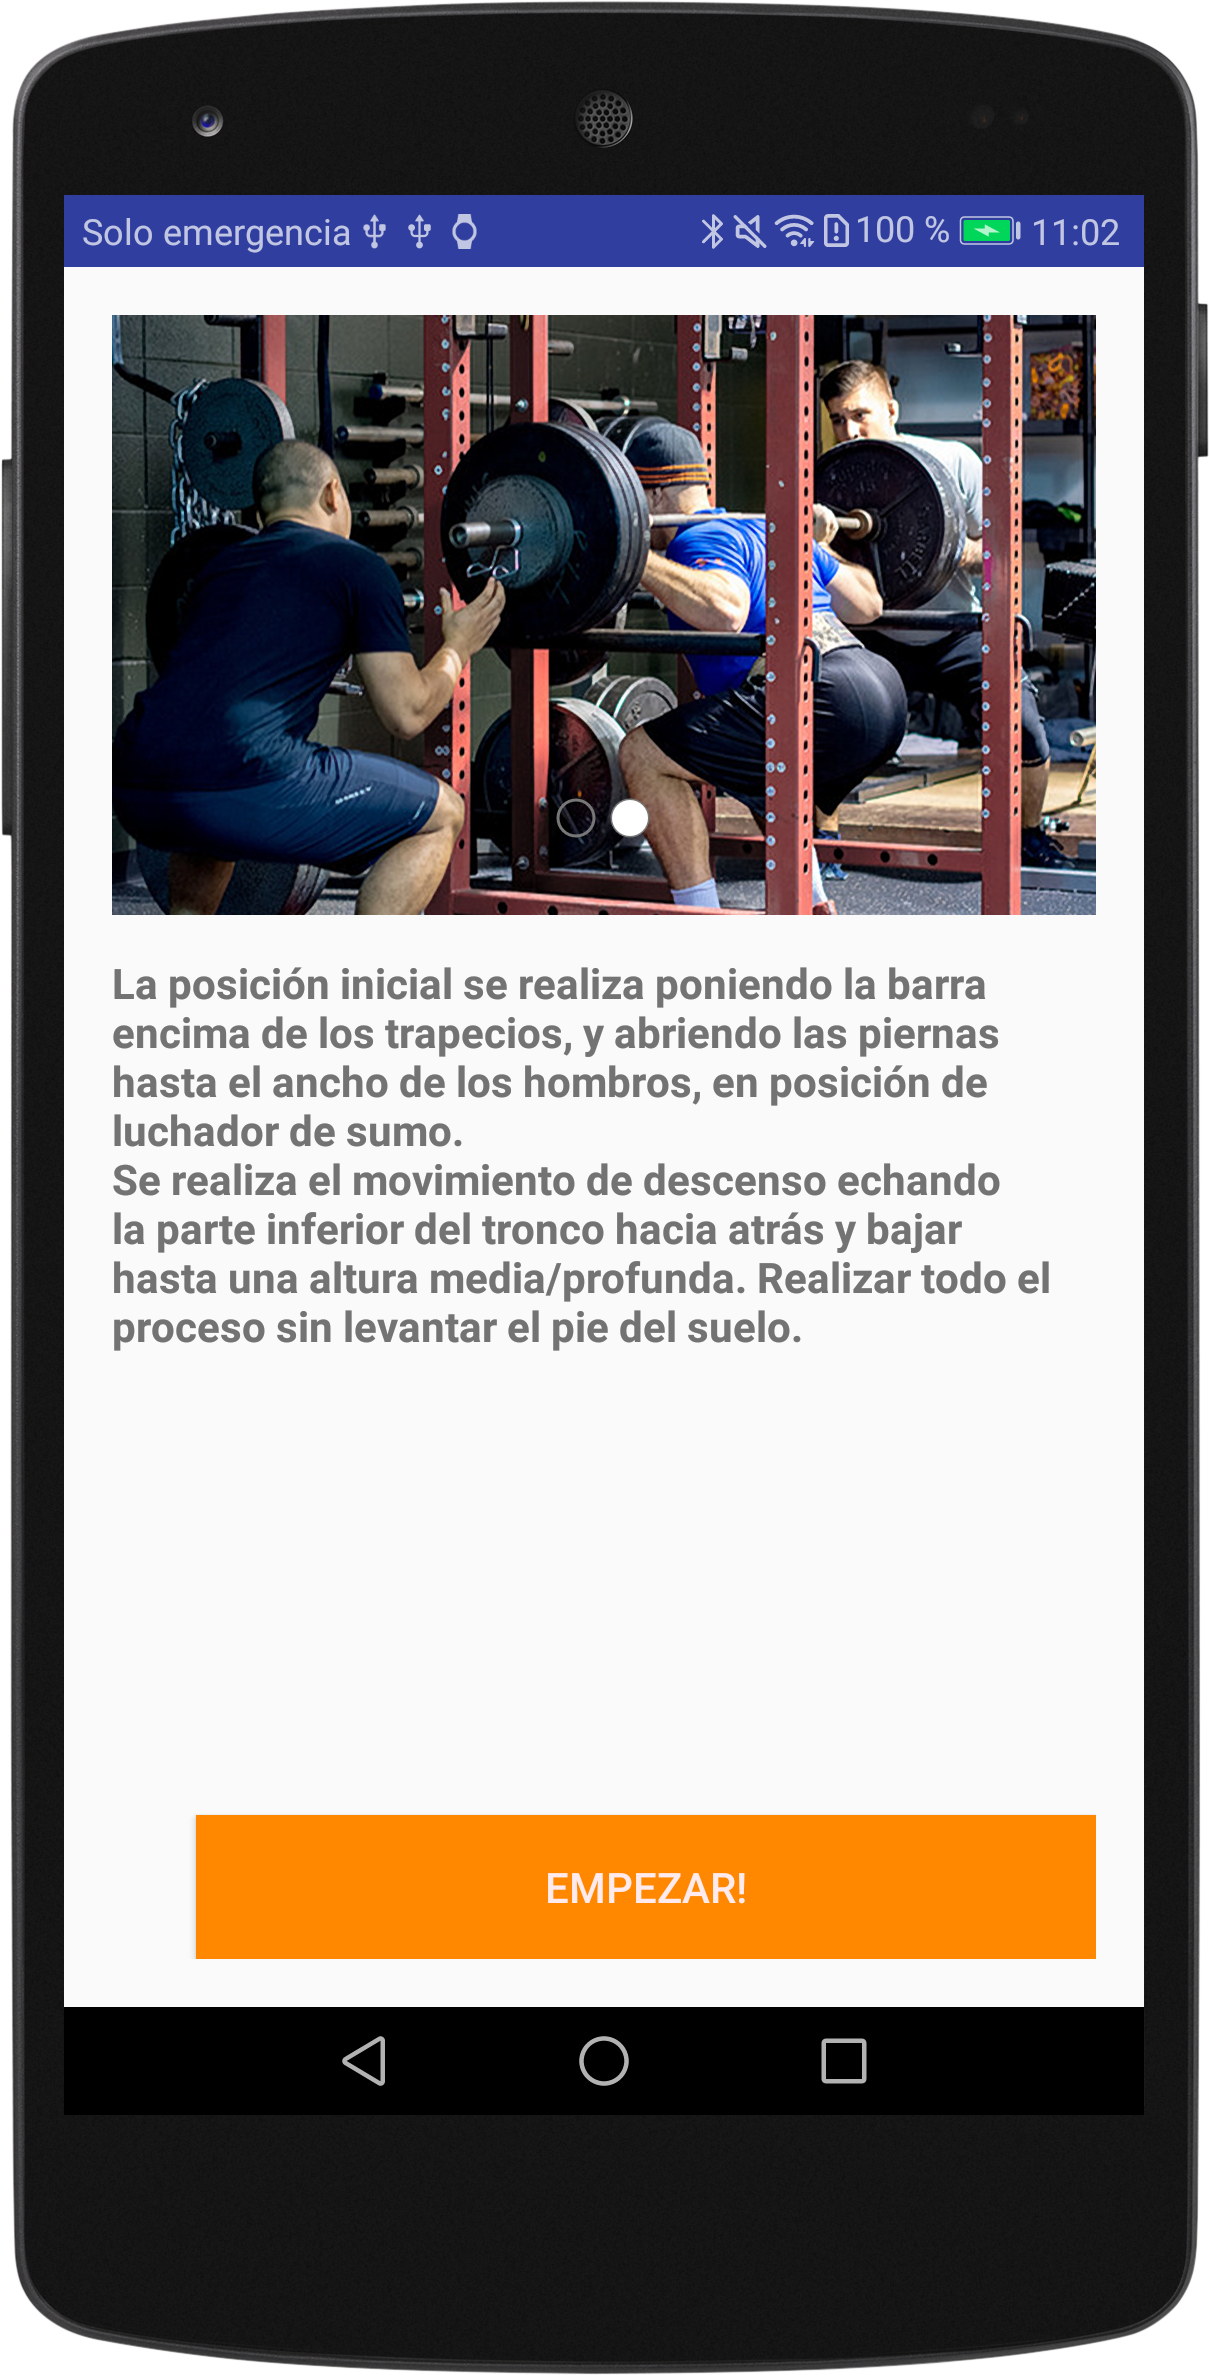
\includegraphics[scale=0.10]{imagenes/m5.png}
	\caption{Ejemplo descripción ejercicio móvil}
	\label{Realización ejercicio 3}
\end{figure}

\begin{figure}[H]
	\centering
	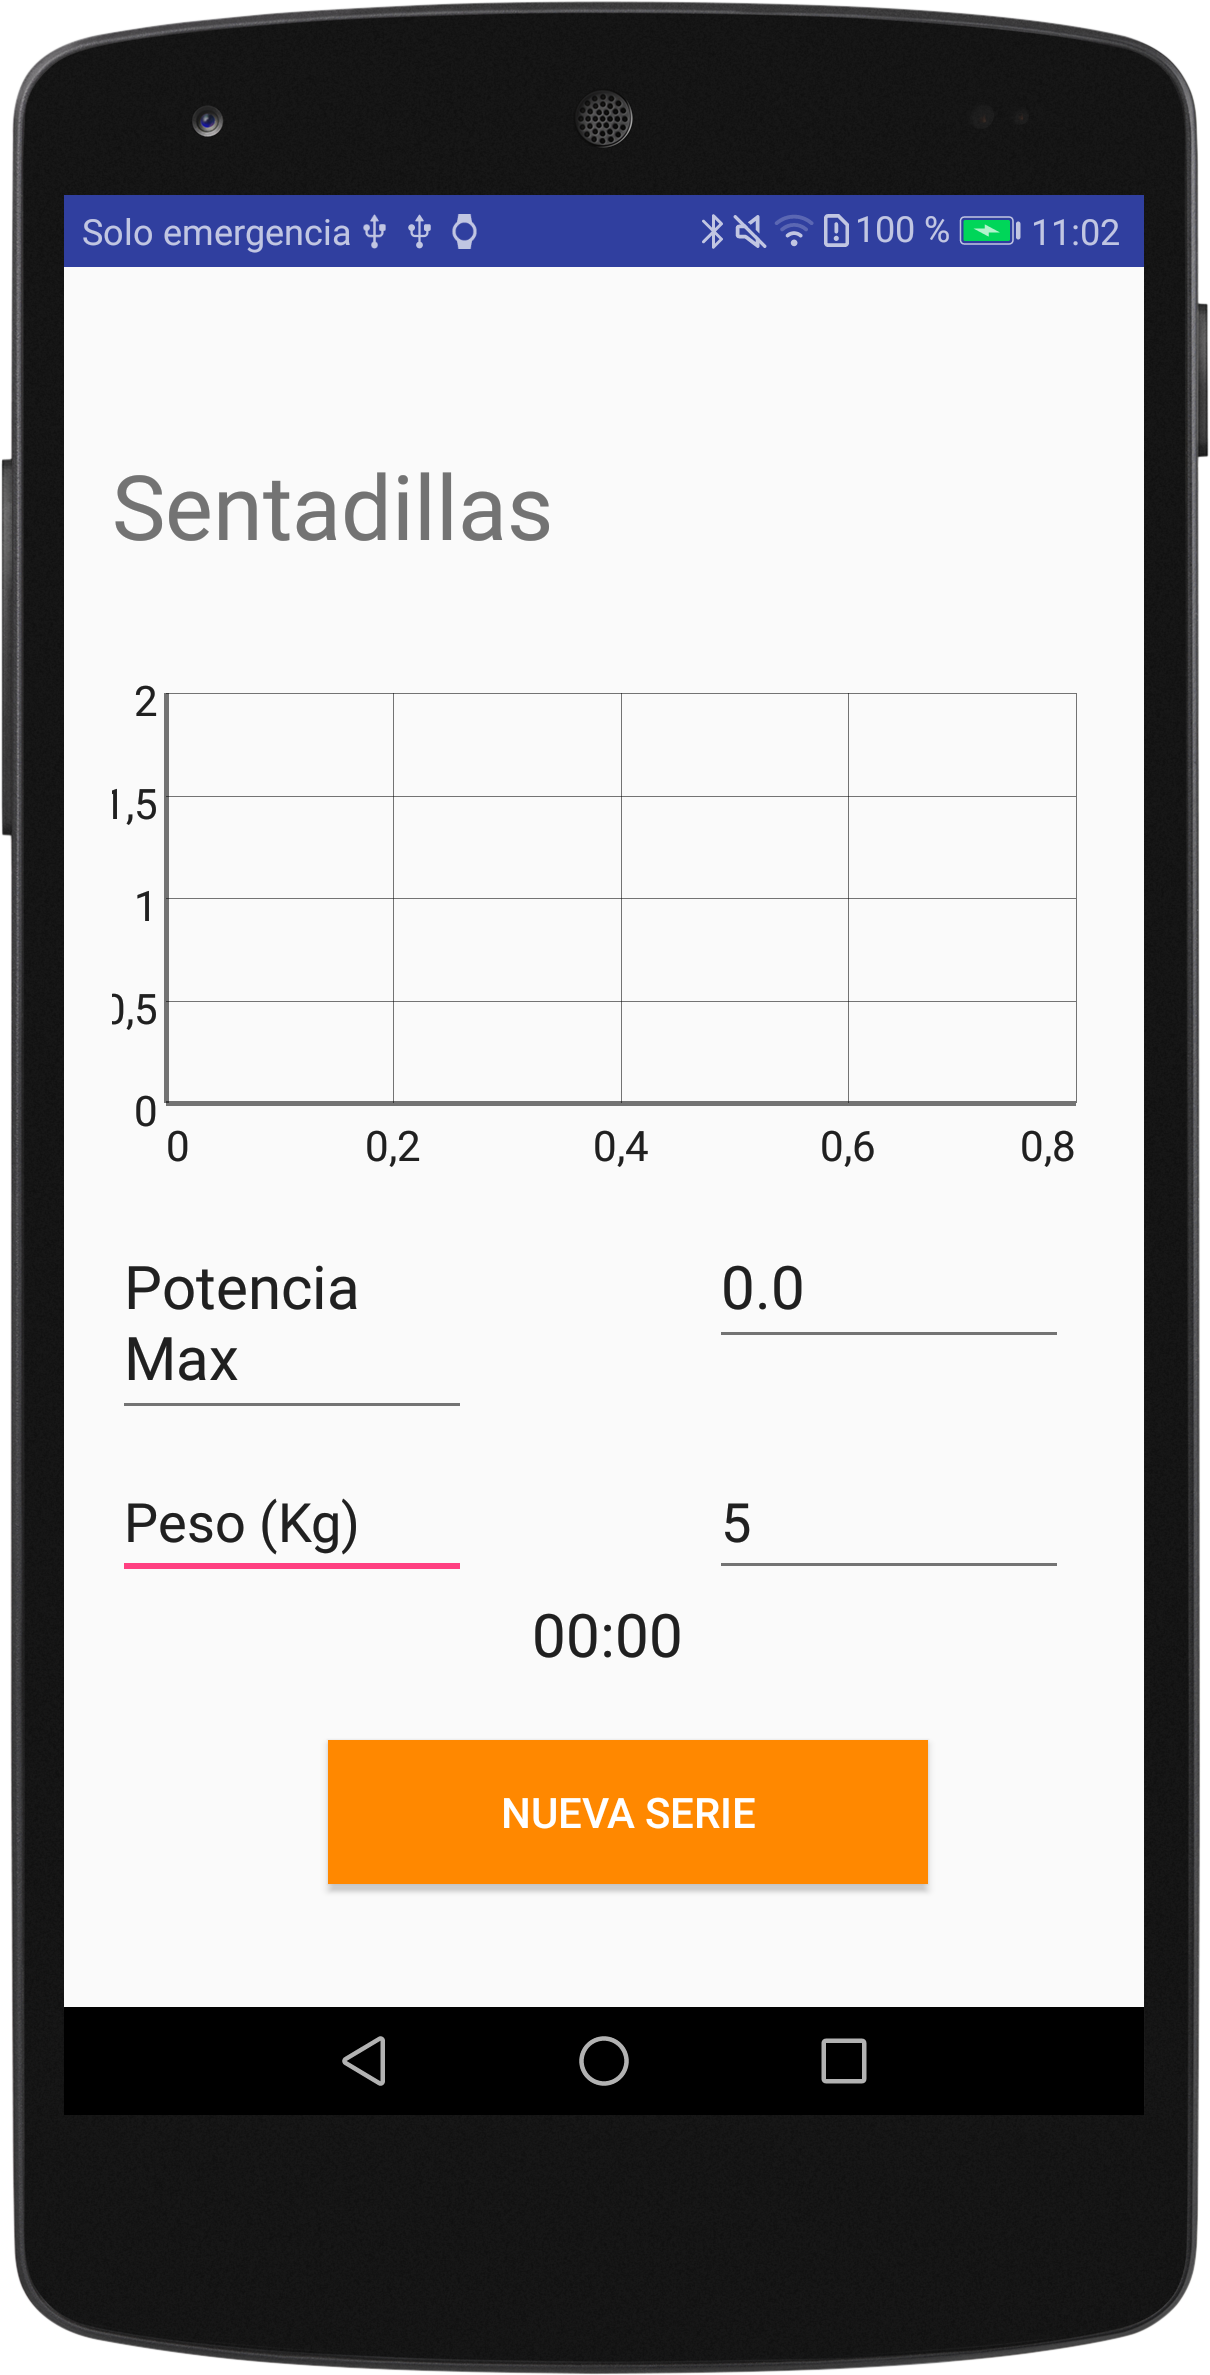
\includegraphics[scale=0.10]{imagenes/m6.png}
	\caption{Ejemplo iniciar ejercicio móvil}
	\label{Realización ejercicio 4}
\end{figure}

Se debe activar la aplicación wear e iniciar el ejercicio:

\begin{figure}[H]
	\centering
	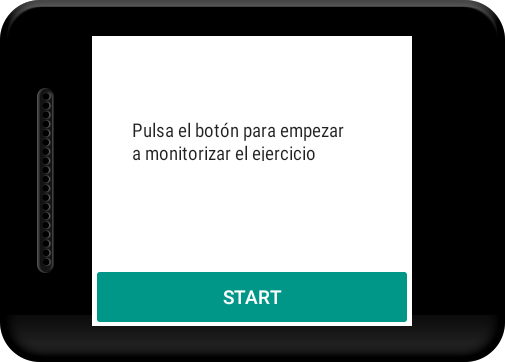
\includegraphics[scale=0.3]{imagenes/w1.png}
	\caption{Pantalla principal wear}
	\label{Realización ejercicio 5}
\end{figure}

\begin{figure}[H]
	\centering
	\includegraphics[scale=0.3]{imagenes/w2.png}
	\caption{Realizar medición wear}
	\label{Realización ejercicio 6}
\end{figure}


Finalmente monitorizando así el ejercicio

\begin{figure}[H]
	\centering
	\includegraphics[scale=0.10]{imagenes/m7.png}
	\caption{Ejemplo realización ejercicio móvil}
	\label{Realización ejercicio 7}
\end{figure}

\section{Consulta del histórico}

Para realizar una consulta simplemente se debe que seleccionar en el menú de navegación la pestaña histórico y seleccionar un día del calendario.

\begin{figure}[H]
	\centering
	\includegraphics[scale=0.10]{imagenes/histori.png}
	\caption{Consulta del histórico}
	\label{Consulta del histórico}
\end{figure}

%%\input{apendices/paper/paper}
%\input{glosario/entradas_glosario}
% \addcontentsline{toc}{chapter}{Glosario}
% \printglossary
\thispagestyle{empty}

\end{document}
